 %%%%%%%%%%%%%%%%%%%%%%% file template.tex %%%%%%%%%%%%%%%%%%%%%%%%%
%
% This is a general template file for the LaTeX package SVJour3
% for Springer journals.          Springer Heidelberg 2010/09/16
%
% Copy it to a new file with a new name and use it as the basis
% for your article. Delete % signs as needed.
%
% This template includes a few options for different layouts and
% content for various journals. Please consult a previous issue of
% your journal as needed.
%
%%%%%%%%%%%%%%%%%%%%%%%%%%%%%%%%%%%%%%%%%%%%%%%%%%%%%%%%%%%%%%%%%%%
%
% First comes an example EPS file -- just ignore it and
% proceed on the \documentclass line
% your LaTeX will extract the file if required
\begin{filecontents*}{example.eps}
%!PS-Adobe-3.0 EPSF-3.0
%%BoundingBox: 19 19 221 221
%%CreationDate: Mon Sep 29 1997
%%Creator: programmed by hand (JK)
%%EndComments
gsave
newpath
  20 20 moveto
  20 220 lineto
  220 220 lineto
  220 20 lineto
closepath
2 setlinewidth
gsave
  .4 setgray fill
grestore
stroke
grestore
\end{filecontents*}
%
\RequirePackage{fix-cm}
%
%\documentclass{svjour3}                     % onecolumn (standard format)
%\documentclass[smallcondensed]{svjour3}     % onecolumn (ditto)
% \documentclass[smallextended]{svjour3}       % onecolumn (second format)
\documentclass[twocolumn]{svjour3}          % twocolumn
%
\smartqed  % flush right qed marks, e.g. at end of proof
%
\usepackage{graphicx}
\usepackage{amsmath}
\usepackage{lmodern}
\usepackage{times}
\usepackage{bm}
\usepackage{mathptmx}
\usepackage{mathrsfs}
\usepackage[sorting=none]{biblatex}  
%\usepackage{biblatex}  
\addbibresource{ref.bib}
\usepackage[justification=centering]{caption}
\usepackage{multicol}
\usepackage{caption}
\usepackage{color}
\usepackage{graphicx}
\usepackage{caption}
\usepackage{graphicx}
\usepackage{float} 
%\usepackage{subfigure}
%\usepackage{subcaption}
% \captionsetup{compatibility=false}

\usepackage{subfig}
\usepackage{graphicx}
\usepackage{epstopdf}
\usepackage{epsfig}
\usepackage{latexsym,bm}        % 处理数学公式中和黑斜体的宏包

\usepackage{amsmath,amssymb}    % AMSLaTeX宏包 用来排出更加漂亮的公式
\makeatletter
\renewcommand\normalsize{%
 \@setfontsize\normalsize\@xpt\@xiipt
 \abovedisplayskip 7\p@ \@plus1\p@ \@minus6\p@
 \abovedisplayshortskip \z@ \@plus3\p@
 \belowdisplayshortskip 8\p@ \@plus3\p@ \@minus3\p@
 \belowdisplayskip \abovedisplayskip
 \let\@listi\@listI}
\makeatother


%
% \usepackage{mathptmx}      % use Times fonts if available on your TeX system
%
% insert here the call for the packages your document requires
%\usepackage{latexsym}
% etc.
%
% please place your own definitions here and don't use \def but
% \newcommand{}{}
%
% Insert the name of "your journal" with
% \journalname{myjournal}
%
\begin{document}
\begin{sloppypar}
\title{EGNet: Enhanced Gradient Network for Image Deblurring%\thanks{Grants or other notes
%about the article that should go on the front page should be
%placed here. General acknowledgments should be placed at the end of the article.}
}
% \subtitle{Do you have a subtitle?\\ If so, write it here}

%\titlerunning{Short form of title}        % if too long for running head

\author{Changdi Zhao         \and
        Xiaoguang Di         \and
        Feng Gao
}

%\authorrunning{Short form of author list} % if too long for running head

\institute{Changdi Zhao \at
              \email{18846144928@163.com}           %  \\
%             \emph{Present address:} of F. Author  %  if needed
          \and
           Xiaoguang Di(corresponding author) \at
              \email{dixiaoguang@hit.edu.cn}
          \and
           Feng Gao \at
              \email{21s104157@stu.hit.edu.cn}
}

\date{Received: date / Accepted: date}
% The correct dates will be entered by the editor


\maketitle

\begin{abstract}
In recent years, convolutional neural networks have been increasingly developed in the field of image deblurring. However, there are still many problems in the existing methods. First, most methods lack attention to the middle layers of the networks, resulting in the lack of gradient information which is important but cannot be restored well by the existing methods. And the ability of the networks which can reconstruct sharp images is reduced. Second, the existing deblurring methods can not perform the self-ensemble of the networks, which has been proved to further improve the network performance in many fields such as image classification and single image super-resolution. Third, the loss function of the existing networks all directly use MAE loss, MSE loss or adversarial loss, which lack the special design for edge information and structural information in the images. To solve the above problems, we enhanced the gradient information of the feature maps after the Encoder in the network, then designed the Self-Ensemble network to further improve the performance, and finally we redesigned the loss function to adaptively redistribute the weight of each position in the gradient map according to the input image. Through the extensive experiments, our proposed method achieve the state-of-the-art results of image deblurring on the existing dataset, and also outperform other methods in generalization ability on RealBlur dataset as well as real blurry images.
\keywords{Image Deblurring\and Enhanced Gradient Network\and Self-Ensemble Network}
% \PACS{PACS code1 \and PACS code2 \and more}
% \subclass{MSC code1 \and MSC code2 \and more}

\end{abstract}

\section{Introduction}
\label{intro}
The objective of image deblurring is to remove the blurry artifacts. Given the input blurry image, it aims to estimate a sharp image which contains more sharp details. And image deblurring can greatly improve the accuracy of other computer vision tasks such as image classification, object detection and semantic segmentation, etc.

The commonly-used blur model is described as Eqn.(1).
\begin{equation}
	    v_{i}  =  k_i \otimes u_{nn(i)} + n_i. \enspace
\end{equation}
Where $v$ is the blurry image, $u$ is the sharp image of size $H \times W$, $k$ is a set of per-pixel blur kernels $k_i$ of size $K \times K$, $\otimes$ represents the convolution operation, $u_{nn(i)}$ represents a window of size $K \times K$ around pixel $i$ in image $u$ and $n_i$ is additive noise\cite{1}.

The traditional non-blind deblurring methods\cite{2} restore the sharp image from the existing blurry image on the premise that the blur kernel $k$ is known. So it cannot be used in practice. In recent years, convolutional neural networks have been further developed, showing superior performance in various computer vision tasks. Nah et al.\cite{3}, Tao et al.\cite{4} and Gao et al.\cite{5}, Zhang et al.\cite{6}, Zamir et al.\cite{7}, Mao et al.\cite{8} and Cho et al.\cite{9} performed the end-to-end image deblurring through a multi-stage and multi-patch neural networks, achieving the state-of-the-art results.

For the existing image deblurring methods based on deep neural networks, there are still many problems that have not been solved. First of all, in each stage, only the Skip-Connection between the Encoder and the Decoder is performed, but the gradient information in the middle feature map which is encoded by the Encoder is missing. Therefore, the deblurring performance of the network is limited. Secondly, the existing methods do not perform the self-ensemble such as averaging multiple results and Geometric Self-ensemble, etc. As a result, the network cannot aggregate the advantages of multiple results simultaneously. Thirdly, MAE Loss or MSE Loss is often used as the content loss or gradient loss. In the calculation process, the pixel-level weight allocation is missing, so it decreases the subjective image quality.

According to the above problems, we have made a series of improvements. Our main contributions are summarized as follows:

(1) We designed an enhanced gradient network to increase the proportion of gradient information in the feature map. Through the network, we can achieve the purpose of adaptively improving the correlation between the feature map and the sharp image. And the enhanced gradient network can be embedded into the existing methods such as MPRNet\cite{7}, DMPHN\cite{6} et al., to further generate more accurate results spatially.

(2) We designed a self-ensemble network to fuse multiple test results, such as the multi-patch test results, the multi-scale test results, etc. And our self-ensemble network can outperform State-Of-The-Art (SOTA) networks in image restoration performance.

(3) We proposed a new loss function, which redistributes the weight of gradient information extracted from different pixels in the image, and the proposed loss function can adaptively improves the proportion of the gradient information in the image. And we can get contextually-enriched results.

(4) Experiments are carried out to verify the generalization ability of the network on the public dataset and the real blurry images captured by our mobile phones. The effectiveness of the enhanced gradient network is verified through the Hilbert Schmidt Independence Criterion(HSIC).\cite{10}. 

\section{Related Work}
\label{sec:1}
During the imaging process, due to the out-of-focus of the imaging device and the relative motion between the objects with the imaging devices, the captured images will contain the blurs, such as the out-of-focus blur, motion blur et al. Existing SOTA learning-based methods\cite{6}\cite{7}\cite{8}\cite{9} directly perform the end-to-end learning through the convolutional neural networks, greatly improving the image restoration performance. Nowadays, the learning-based image deblurring methods can be classified into three categories,i. e. CNN-based methods, GAN-based methods and self-ensemble methods.

{\bfseries CNN-Based methods.} Carbajal et al.\cite{1} proposed a general nonparametric model for dense non-uniform motion blur estimation. Zhang et al.\cite{6} did not use the multi-scale input at different stages, but used multi-patch input at different stages to improve the deblurring effect for small objects. Zamir et al.\cite{7} continued the idea of multi-scale network and multi-patch network, and introduced an attention mechanism in the fusion process of each stage. Quan et al.\cite{11} proposed a single image defocus deblurring network by unrolling a fixed-point iteration derived from a GKM-based model of defocus blurring process. Quan et al.\cite{12} proposed a non-blind image deblurring approach which is built upon the unfolded optimization of a deconvolution model equipped with a Gabor-domain denoising prior. Chen et al.\cite{13} proposed a dataset-free approach which is not dependent on external training dataset. Quan et al.\cite{14} developed a scheme of constructing non-local wavelet frame and tight frame which are adaptive to the input image.  However, these methods do not consider the gradient information in the feature maps of the intermediate layers, so the deblurring results contain over-smooth contents. Therefore, the network performance is limited.

{\bfseries GAN-Based methods.} On the basis of WGAN\cite{15}\cite{16}, Kupyn et al.\cite{17} only used adversarial loss and perceptual loss to train their network DeblurGAN. Since it does not directly use MAE loss or MSE loss, it has a poor performance on PSNR. To solve this problem, Kupyn et al.\cite{18} made further improvements and proposed the DeblurGAN-v2. They combined the rich semantic information among the feature maps with different resolution. And they proposed a new loss function RaGAN-LS loss. It combines the existing MSE loss and perceptual loss, so the restored image with both high PSNR and high SSIM is obtained. But in general, the images generated by GAN-based methods often have some artifacts.

{\bfseries Self-Ensemble methods.} The self-ensemble method can not be applied well in the existing deblurring methods. But in the image classification task, the aggregation of multiple results through the multi-scale and multi-crop testing, random horizontal flipping\cite{19}\cite{20} can effectively improve the accuracy of the model. When it is used to the image deblurring, the restored image will contain overly smooth contents and artifacts. In single-image super-resolution, Geometric Self Ensemble\cite{21} uses a single trained model to obtain 8 augmented inputs by flipping and rotation. And the average are performed to obtain the final result, which can effectively improve the performance. But it is only valid for symmetric downsampling methods. So it can not be applied to image deblurring directly. Chen et al.\cite{22} proposed an ensemble approach to exploit the priors from untrained neural network for blind image deblurring, which aggregates the deblurring results of multiple untrained neural network for improvement. In \cite{23}, the prediction is done by averaging over the estimates from both perturbed the images and kernels. These methods use kernels to maintain the consistency of noise characteristics between the training and test process, whitch limits the generalization ability and robustness of the deblurring network.

There are some problems in the existing deblurring methods. Most of the methods use Encoder-Decoder network directly and do not consider the gradient information in the intermediate feature maps, so the deblurring results contain overly smooth contents. And the deblurring network can not directly use the existing self-ensemble methods to boost the network performance. Our proposed network can effectively increase the proportion of gradient information in the intermediate feature map and the proposed self-ensemble network can boost the network deblurring performance.

\section{Proposed Method}
\begin{figure}[h]
\centering
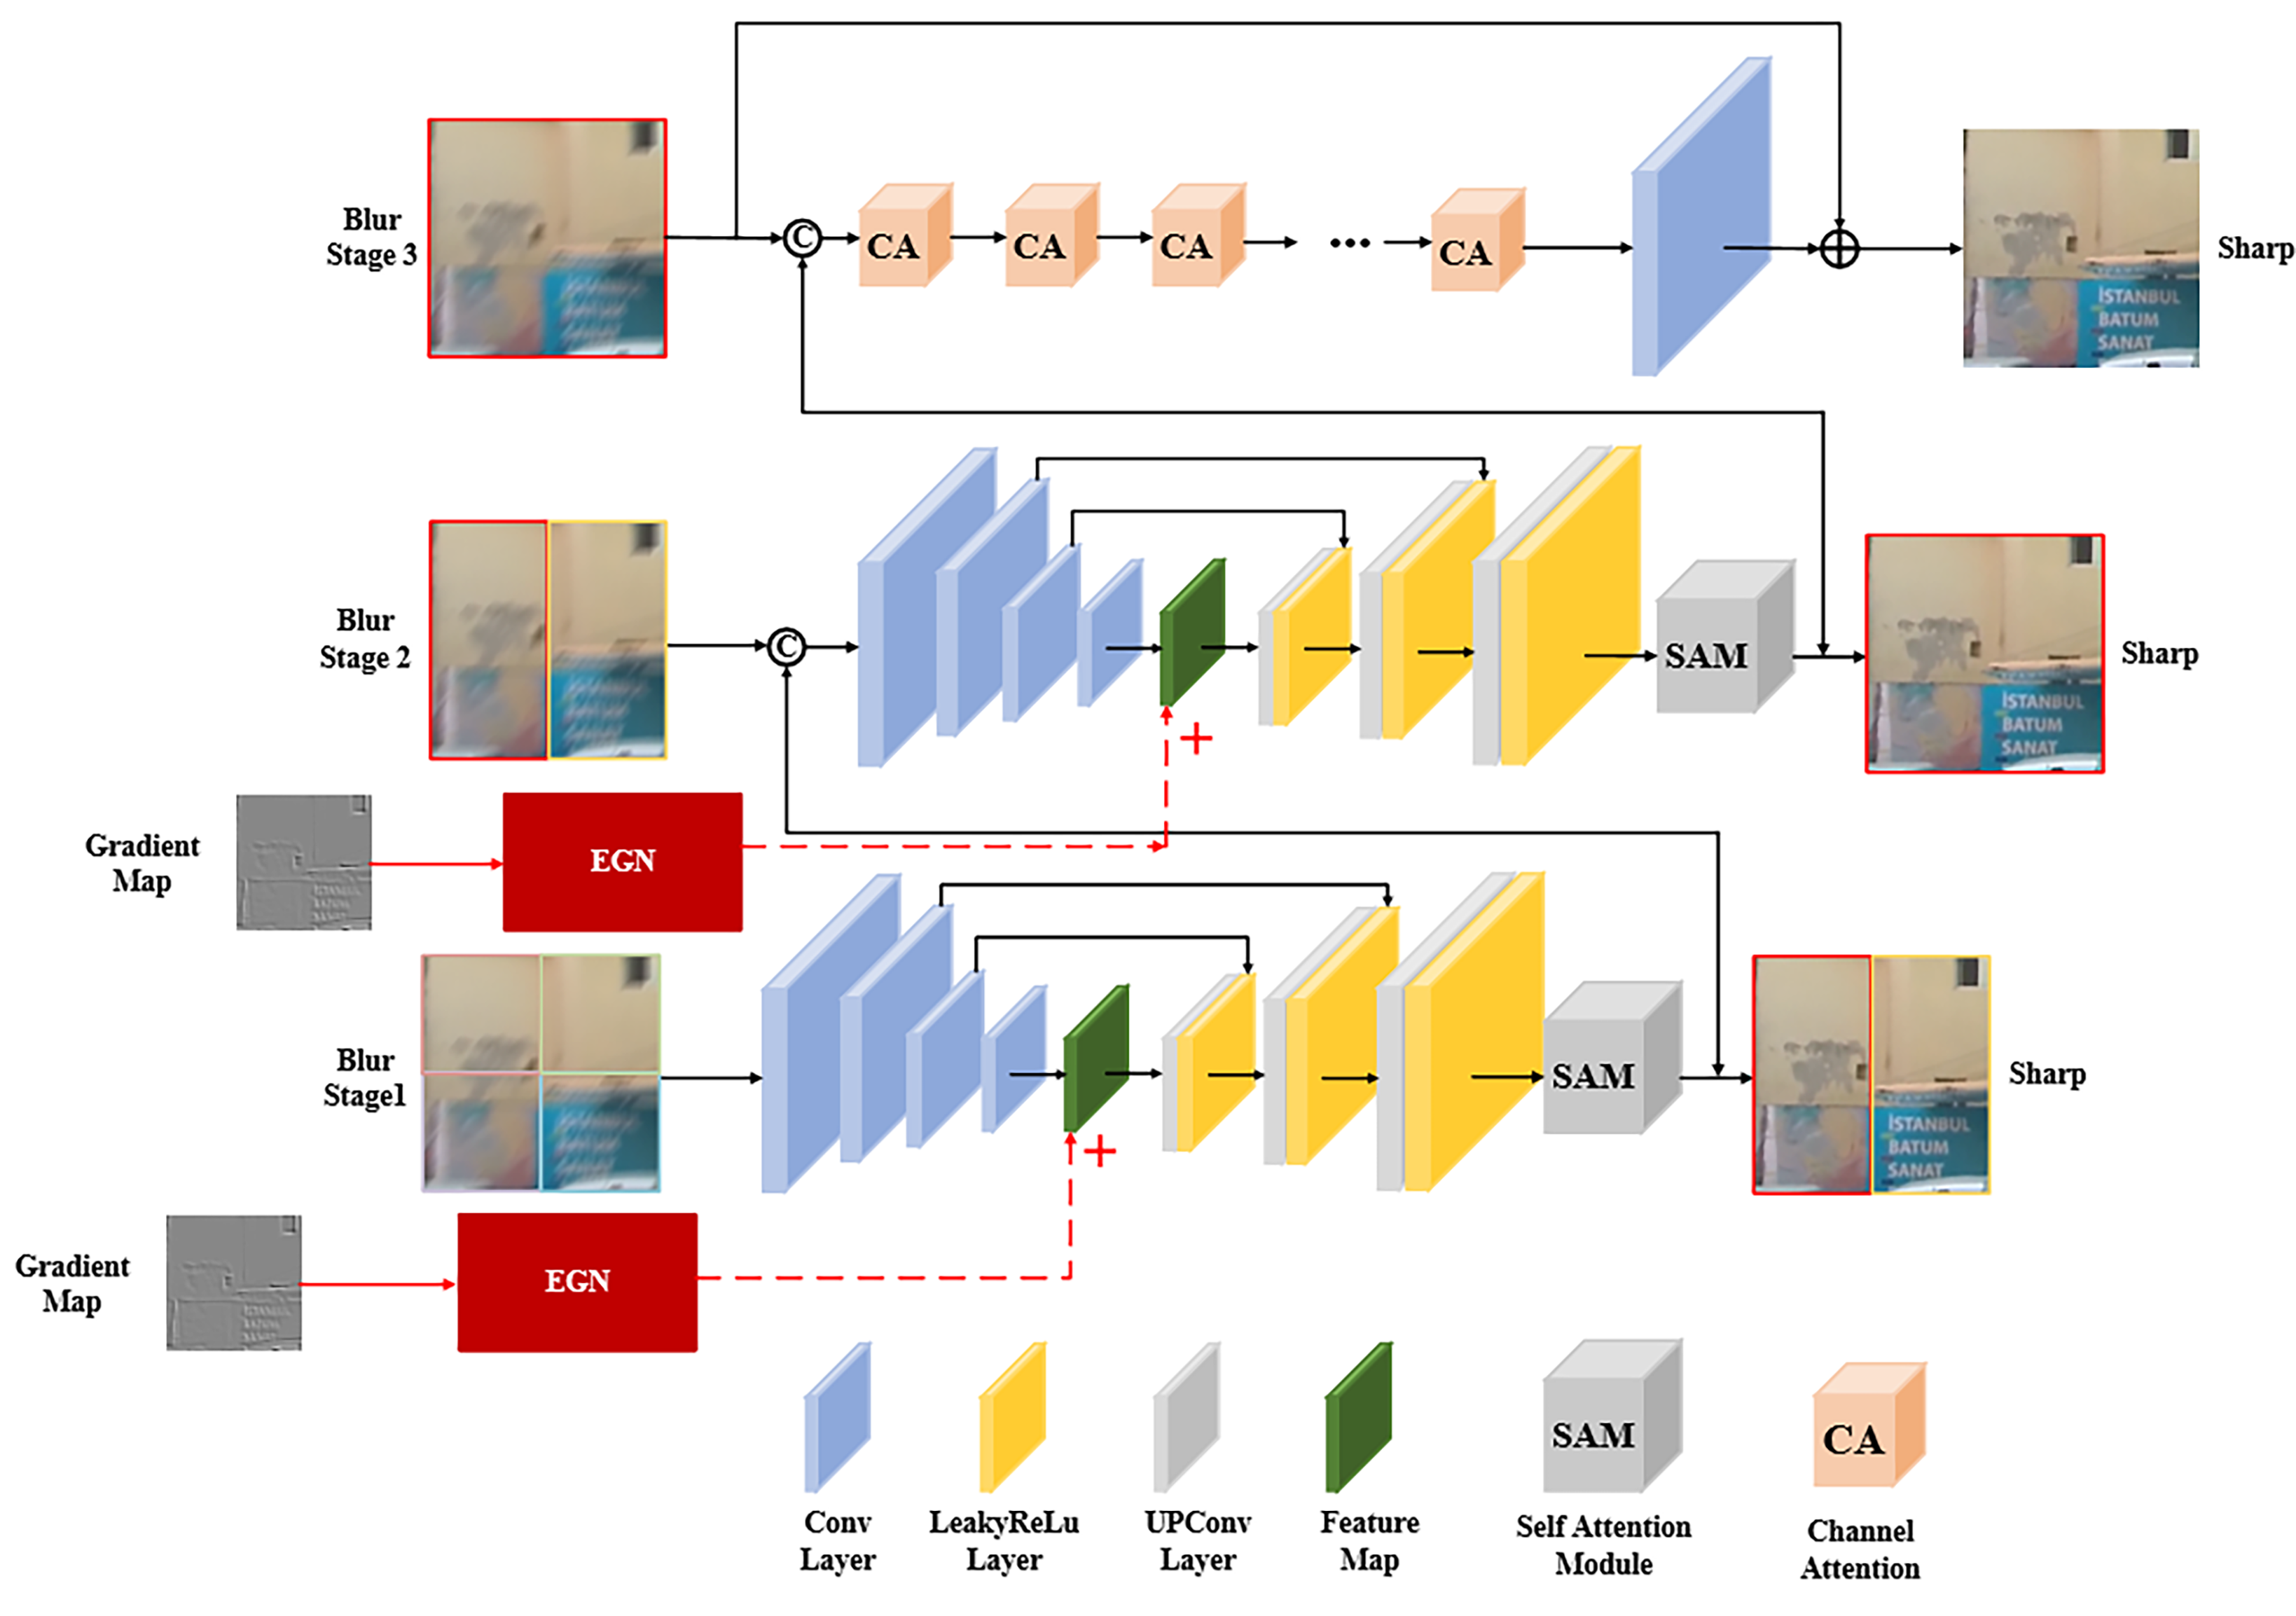
\includegraphics[width=8cm]{images/fig1.png}
\caption{The overall architecture of our proposed method.}
\label{fig_sim}
\end{figure}
The overall framework of our image deblurring network consists of three stages to progressively restore the images, as shown in Figure 1. The first two stages are based on encoder-decoder subnetworks that learn the broad contextual information due to large receptive fields. And the last stage employs a subnetwork without any downsampling operation. The input and output of the three stages are blurry images and restored images, respectively. We adapt the multi-patch hierarchy on the input image and split the image into non-overlapping patches: four for stage-1, two for stage-2, and the original image for the last stage, as shown in Fig.1.

In addition, instead of simply using Encoder-Decoder subnetworks, we incorporate an Enhanced Gradient Network between the encoder and decoder, that increases the proportion of gradient information in the feature map, which will be detailed in Subsection 3.1. On this basis, we adopt a variety of test methods, mainly from the
following aspects: 1) input the blurry image which is downsampled -- image deblurring -- output the restored image and the up-sampling; 2) input the blurry image -- image deblurring -- output the restored image; 3) input the blurry image which is splited into four non-overlapping patches -- image deblurring -- output the restored patches. And these test methods are used in Subsection 3.2. As for the loss function, we propose a new gradient loss in Subsection 3.3. Next, we describe each key element of our method.
\begin{figure}[h]
\centering
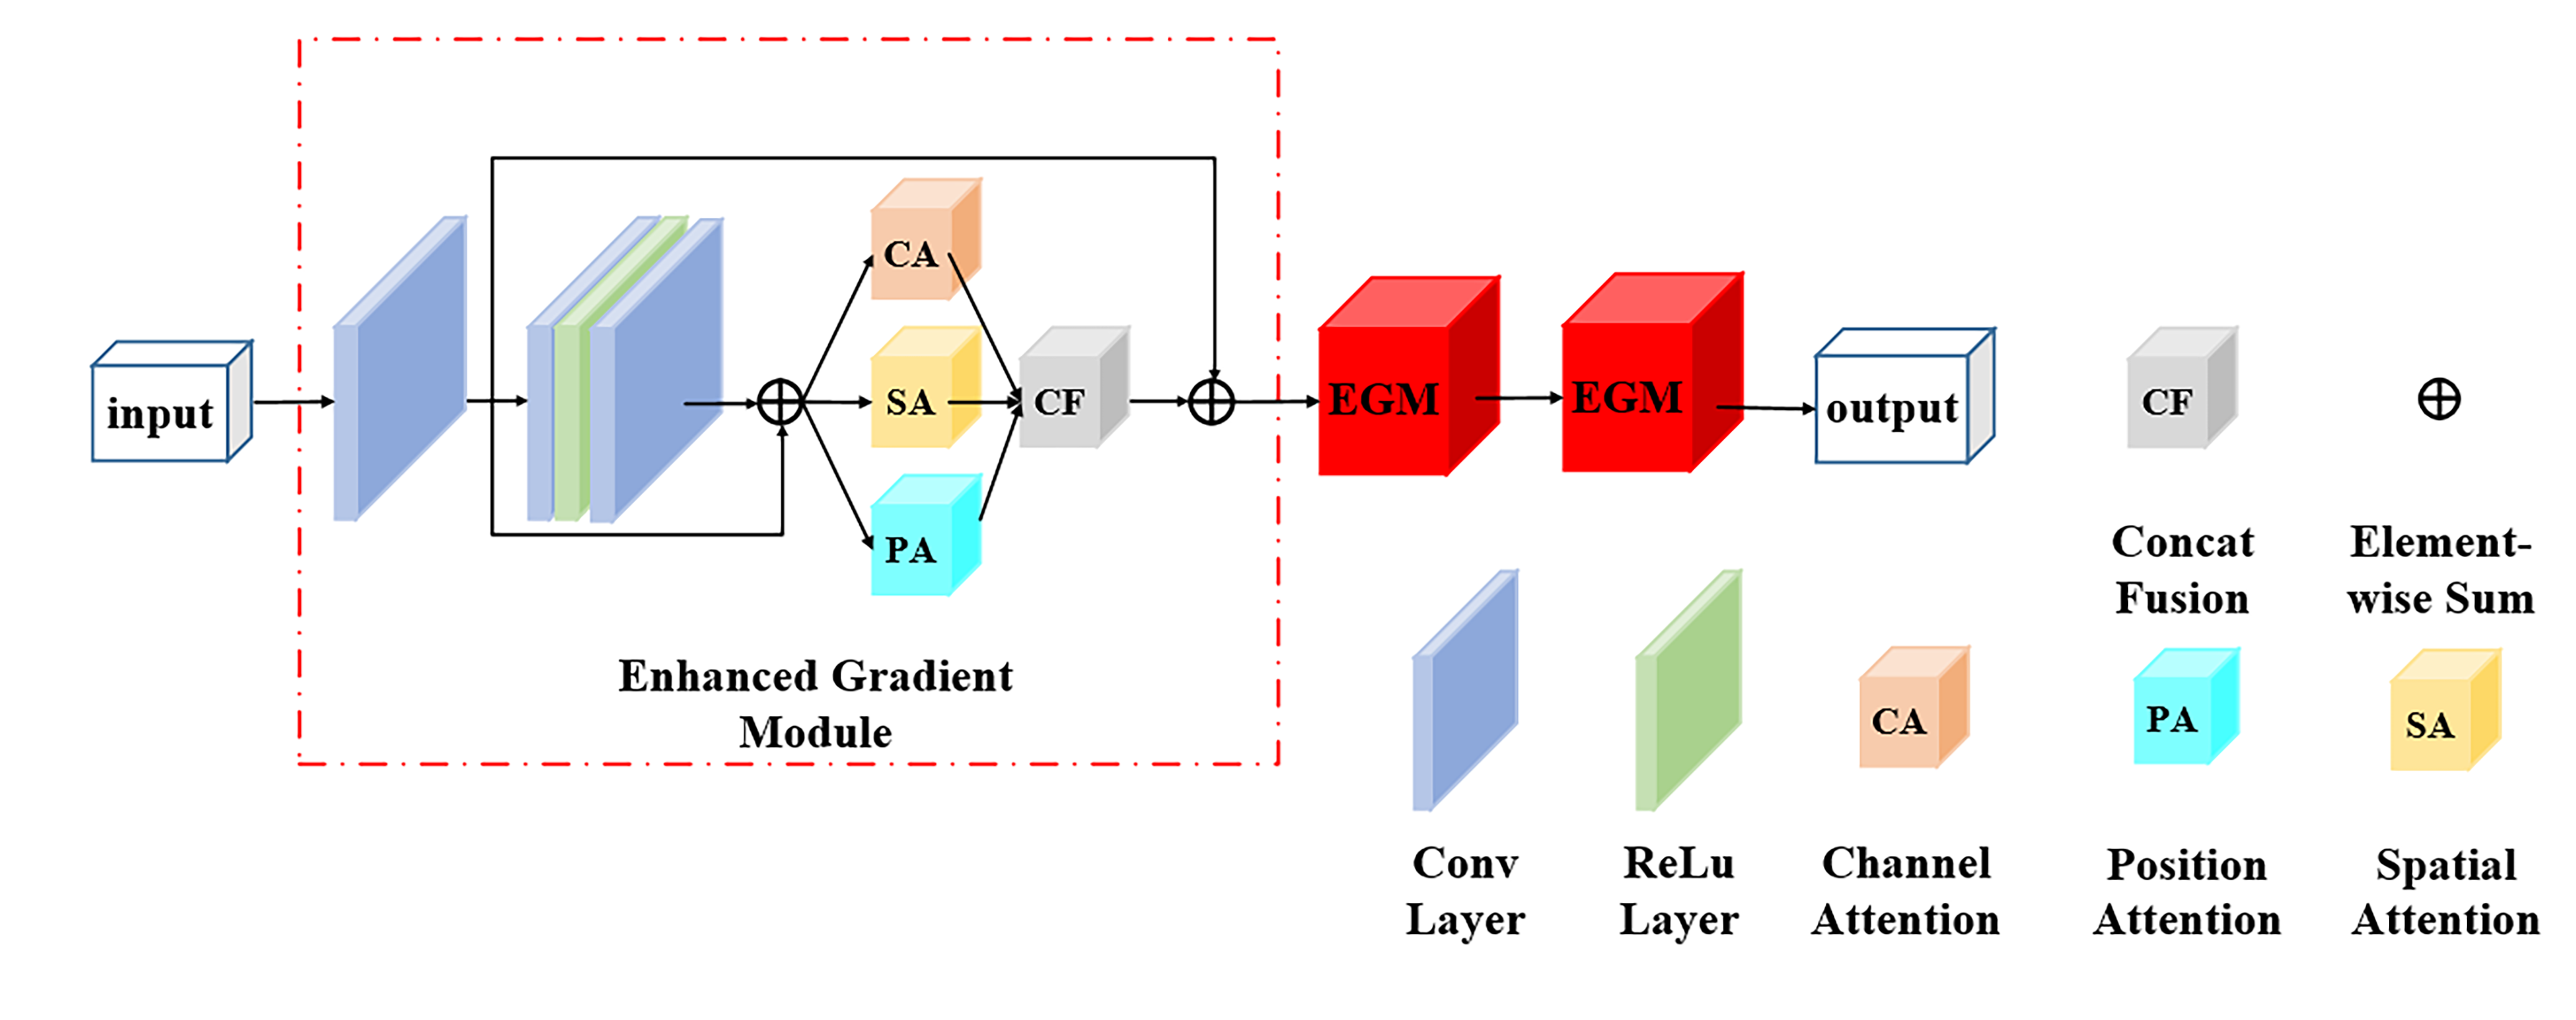
\includegraphics[width=8cm]{images/fig2.png}
\caption{Enhanced Gradient Network.}
\label{fig_sim}
\end{figure}
\subsection{Enhanced Gradient Network}
The Enhanced Gradient Network(EGN) is shown in Figure 2. In the stage-1 and stage-2 of the network, in addition to taking the blurry image as input, the gradient map of the image is also put into the Enhanced Gradient Network. By doing this, we can improve the proportion of gradient information in the feature map which is obtained by the Encoder.

\subsubsection{Enhanced Gradient Module}
EGN includes several Enhanced Gradient Modules(EGMs). The structure of EGM is shown in Figure 2. Here, we use residual channel attention module and residual spatial attention module\cite{24} to learn the channel and pixel weights of the features. Further, we exploit the position attention module to enhance the local feature correlation among the feature maps. We experimentally demonstrate that these attention modules boost the performance as detailed in Sec. 4.

\subsubsection{Residual Channel Attention}
The Residual Channel Attention(RCA) module is shown in Figure 3. The input of RCA module goes through successive convolutional layers to get $x^{in_1}$ $\in$ $R^{H \times W \times C}$, as shown in Eqn.(2). Where $in_1$ represents the input to the module of weight distribution, ${H \times W}$ denotes the spatial dimension and $C$ represents the number of channels.
\begin{equation}
	    x^{in_1}  =  C_2(R(C_1(x^{in}))). \enspace
\end{equation}
Where $C_1$ and $C_2$ represent the convolutional layers in RCA module. $R$ represents the activation layer.

Next, we redistribute the weight of each channel of $x^{in_1}$. As shown in Eqn.(3), after we get the feature map of the residual branch, we add it with the input $x^{in}$ to get the final result $x^{out}$.
\begin{equation}
	    x^{out}  =  x^{in} + x^{in_1} * C_4(R(C_{c3}(GA(x^{in_1})))). \enspace
\end{equation}
Where GA represents Global Average Pooling. $C_{c3}$ and $C_4$ represent the third and the fourth convolutional layers in RCA module, respectively. $*$ represents element-wise product.
\begin{figure}[h]
\centering
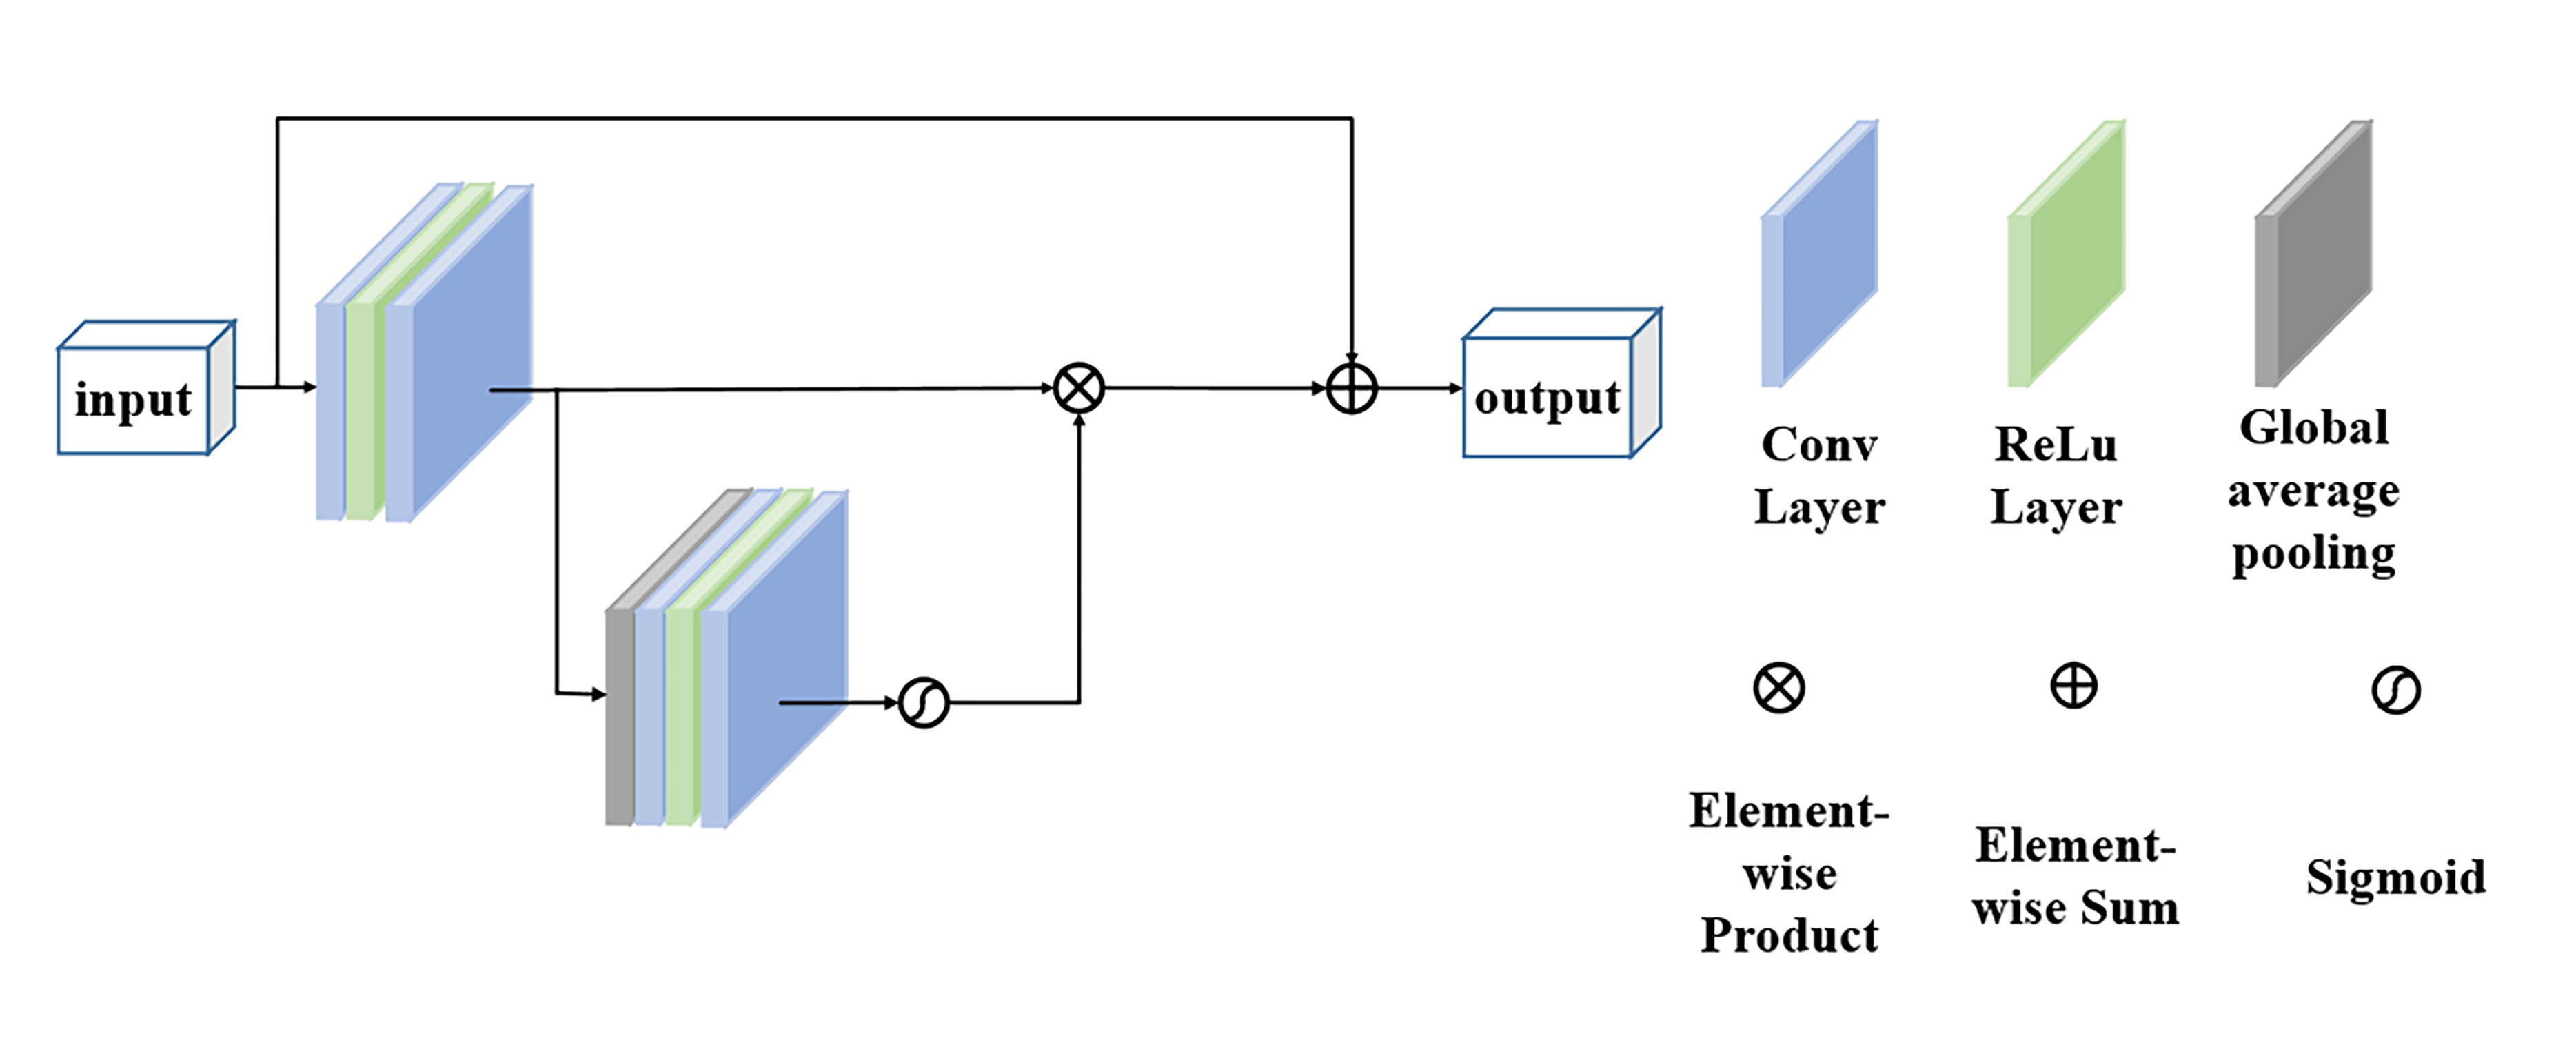
\includegraphics[width=8cm]{images/fig4.png}
\caption{Residual Channel Attention Module.}
\label{fig_sim}
\end{figure}
\subsubsection{Residual Spatial  Attention}
In Residual Spatial Attention(RSA) module, as shown in Figure 4, we can get $x^{in_1}$ like the RCA module. Then we redistribute the pixel weights and increase the pixel weights that are conducive to image restoration. As shown in Eqn.(4), $x^{in_1}$ is sent to an average pooling layer and a max pooling layer to get $A$ $\in$ $R^{H \times W \times 1}$ and $M$ $\in$ $R^{H \times W \times 1}$. We can get the weight coefficient for each pixel by sending the concatenation of $A$ and $M$ to a convolutional layer and a sigmoid activation function.
\begin{equation}
	    x^{out}  =  x^{in} + x^{in_1} * \sigma(C_{s3}(Cat(AP(x^{in_1}), MP(x^{in_1})))). \enspace
\end{equation}
Where $C_{s3}$ represents the third convolutional layer in RSA module. $Cat(a,b)$ represents the concatenation of $a$ and $b$. $AP$ and $MP$ represent the average pooling layer and the max pooling layer respectively. $\sigma$ represents the sigmoid activation function.
\begin{figure}[h]
\centering
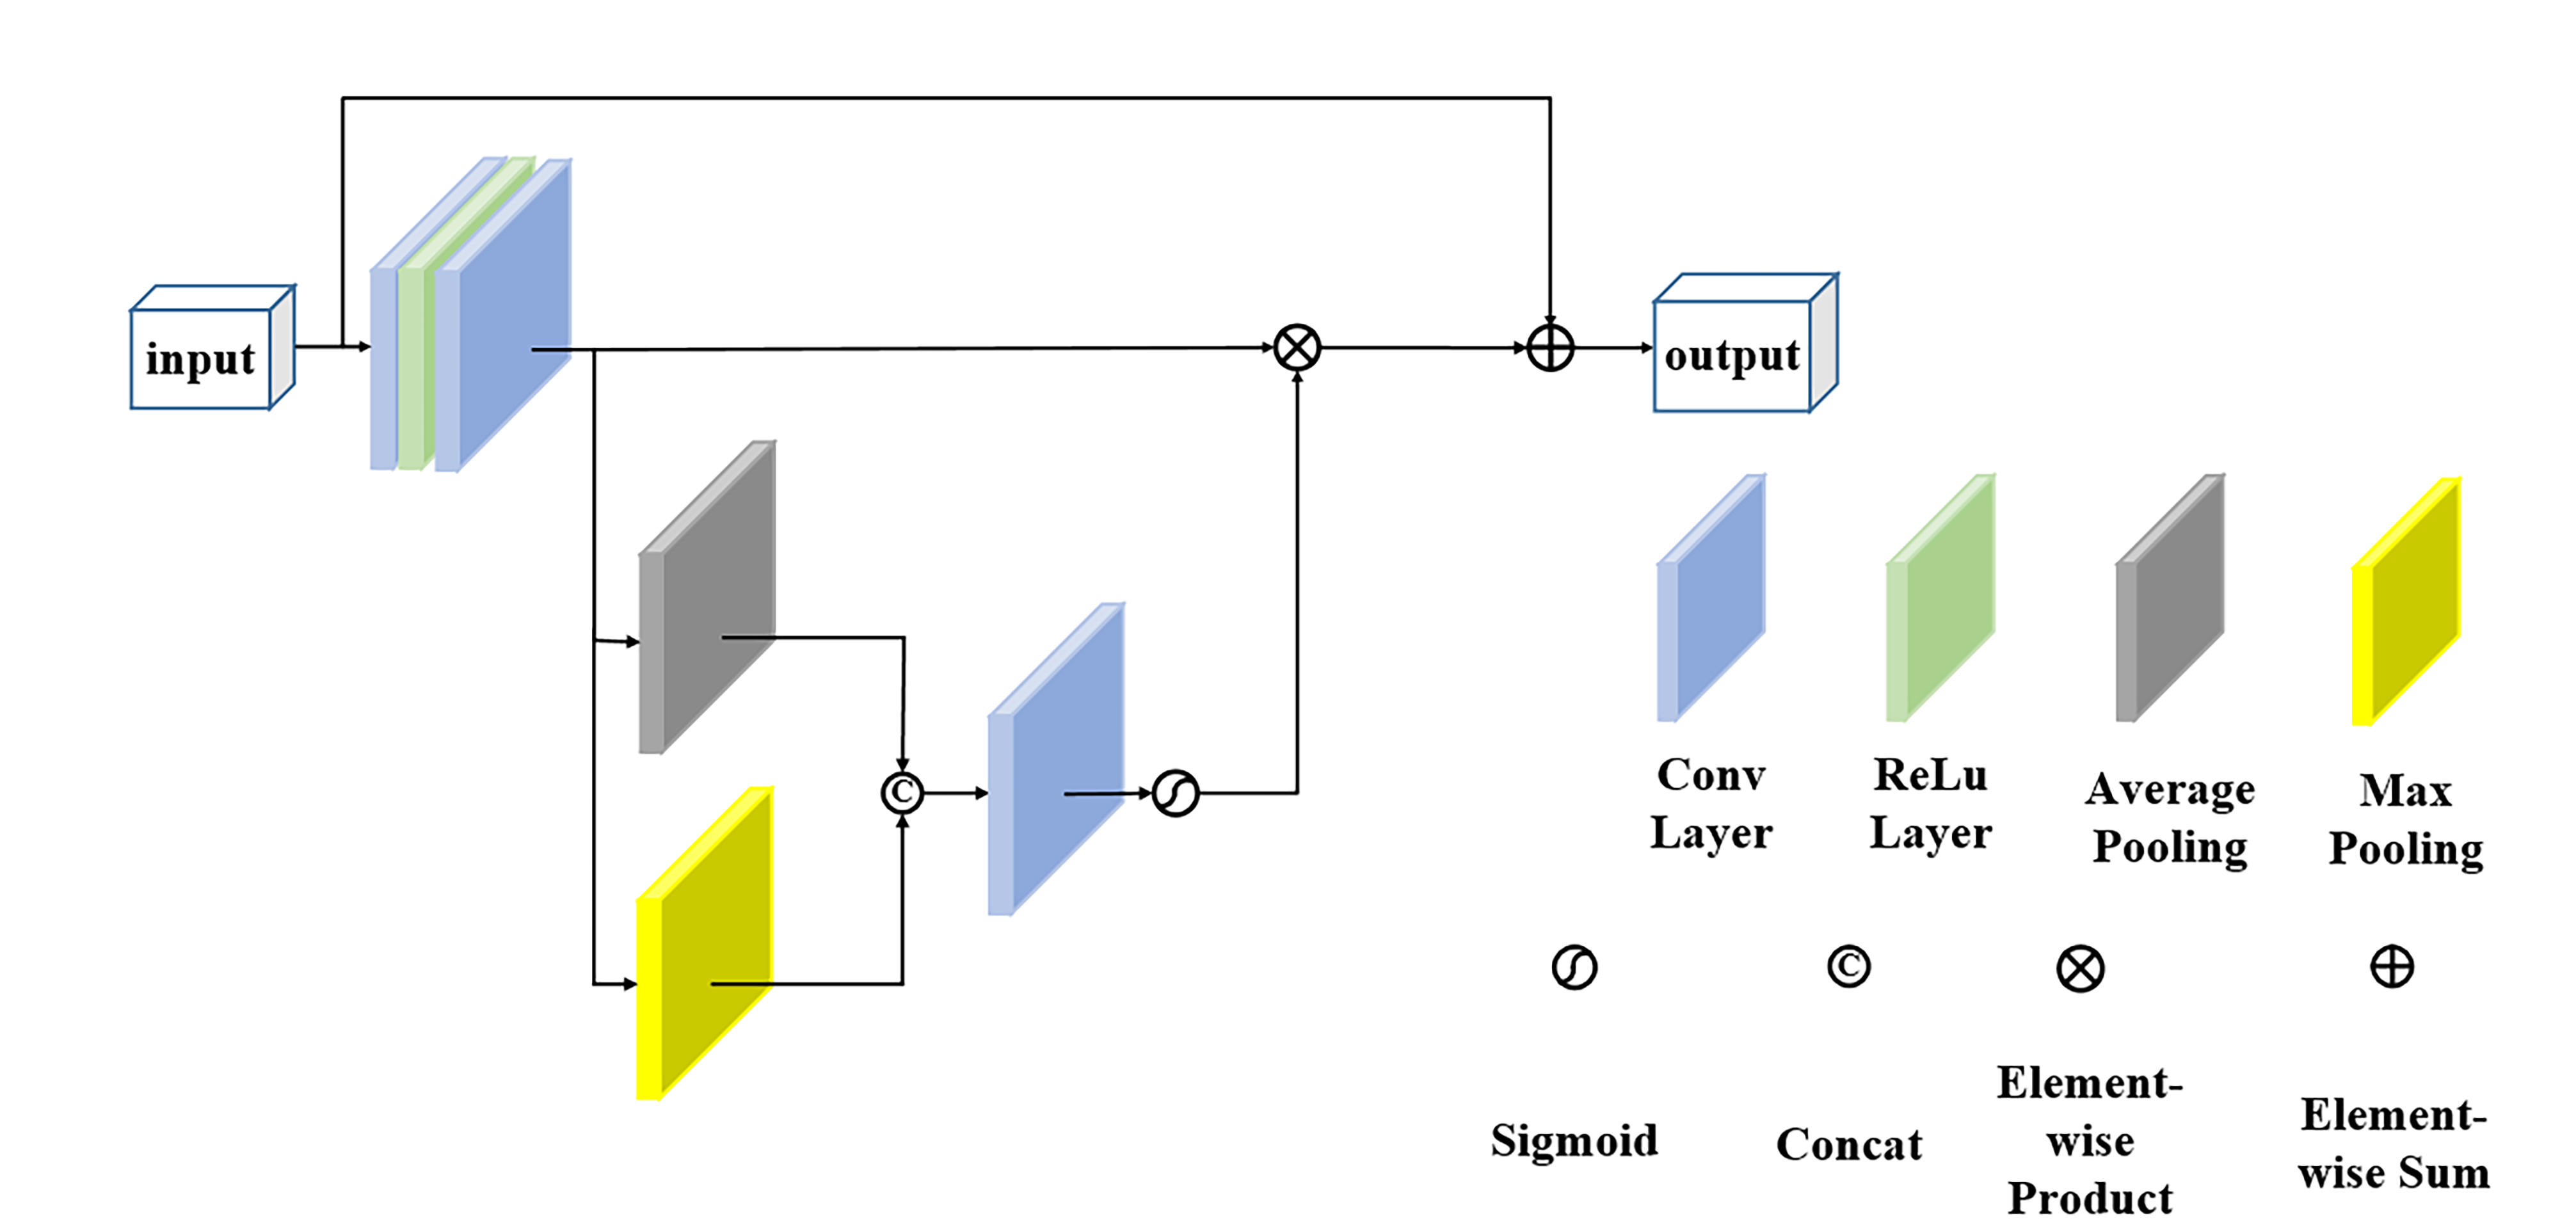
\includegraphics[width=8cm]{images/fig5.png}
\caption{Residual Spatial Attention Module.}
\label{fig_sim}
\end{figure}
\begin{figure}[h]
\centering
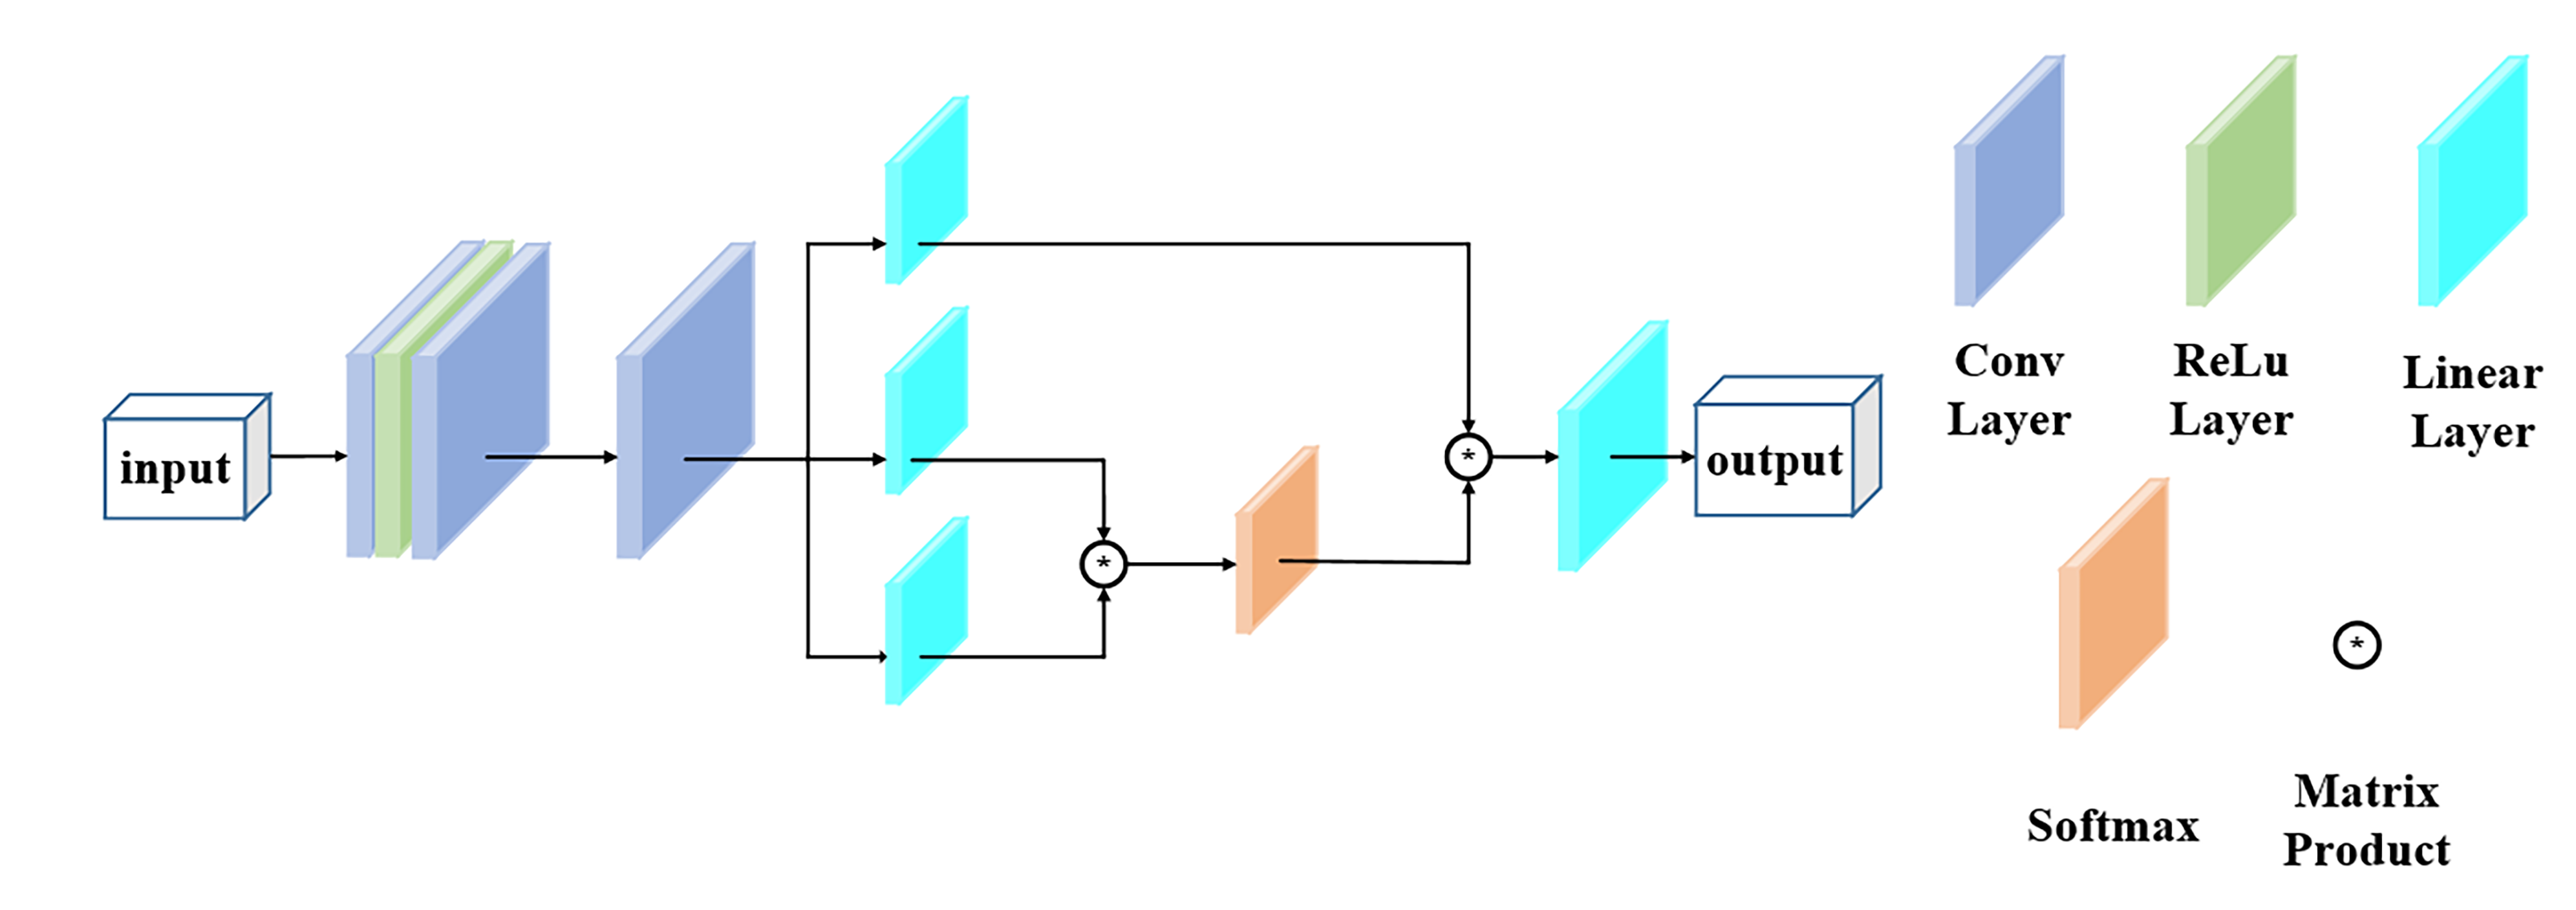
\includegraphics[width=8cm]{images/fig6.png}
\caption{Position Attention Module.}
\label{fig_sim}
\end{figure}
\subsubsection{Position Attention}
In the Position Attention(PA) Module, as shown in Figure 5, $x^{in_1}$ $\in$ $R^{H \times W \times C}$ is reshaped to $R^{HW \times C}$. And we can get $q$ $\in$ $R^{HW \times C_1}$, $k$ $\in$ $R^{C_1 \times HW}$ and $v$ $\in$ $R^{HW \times C_2}$ by three linear layers. Then we can get coefficient matrix $z$ $\in$ $R^{HW \times HW}$ by the matrix multiplication between $q$ and $k$. The coefficient matrix $z$ and $v$ are multiplied to get the output $v$ $\in$ $R^{HW \times C_2}$. Finally, we get the output $x^{out}$ $\in$ $R^{H \times W \times C}$ by a linear layer and the reshaping operation(as shown in Eqn.(5)-(9)).
\begin{equation}
	    q  =  L_1(C_{p3}(x^{in_1})). \enspace
\end{equation}
\begin{equation}
	    k  =  L_2(C_{p3}(x^{in_1})). \enspace
\end{equation}
\begin{equation}
	    v  =  L_3(C_{p3}(x^{in_1})). \enspace
\end{equation}
\begin{equation}
	    z  =  SM(MUL(q, k)). \enspace
\end{equation}
\begin{equation}
	    x^{out}  =  L_4(MUL(z, v)). \enspace
\end{equation}
Where $C_{p3}$ represents the third convolutional layer in PA module. $L_1$, $L_2$, $L_3$, $L_4$ represent the four linear layers in PA module. $MUL$ represents the matrix multiplication. $SM(a)$ represents the softmax result of $a$.
\subsection{Self-Ensemble Network}

After obtaining a variety of test results, such as the output obtained by downsampling, the output obtained by the original image, etc, we find that simply averaging multiple test results cannot effectively combine edges of the test results and may have checkerboard artifacts. Therefore, it is necessary to design a Self-Ensemble network. We can obtain the final result through a Self-Ensemble Network, which aims to combine the advantages of various test results.

As shown in Figure 6, the Self-Ensemble network is a multi-branch channel attention network. The multiple input images of the network are $I_1$, $I_2$, $I_3$…$I_n$. The image $I_i$ is passed through a residual block to obtain the feature map $I_{i_1}$, which is described as Eqn.(10).
\begin{equation}
	    I_{i_1}  =  I_i + C_2(R(C_1(I_i))). \enspace
\end{equation}
The feature maps of each branch are added and passed through several convolutional layers and Softmax layers(as shown in Eqn.(11)). $z_{in}$ $\in$ $R^{H \times W \times n}$ is used as the input of Softmax layer, and the weight coefficients of different branches are obtained after the softmax operation(as shown in Eqn.(12)).
\begin{equation}
	    z_{in}  =  C_5(R(C_4(R(C_3(\sum_{i=1}^{n}I_{i_1}))))). \enspace
\end{equation}
\begin{equation}
	    z_{out}^{i,j,c}  =  \frac{exp(z_{in}^{i,j,c})}{\sum_{m=1}^{n}{exp(z_{in}^{i,j,m})}}. \enspace
\end{equation}
\begin{figure}[h]
\centering
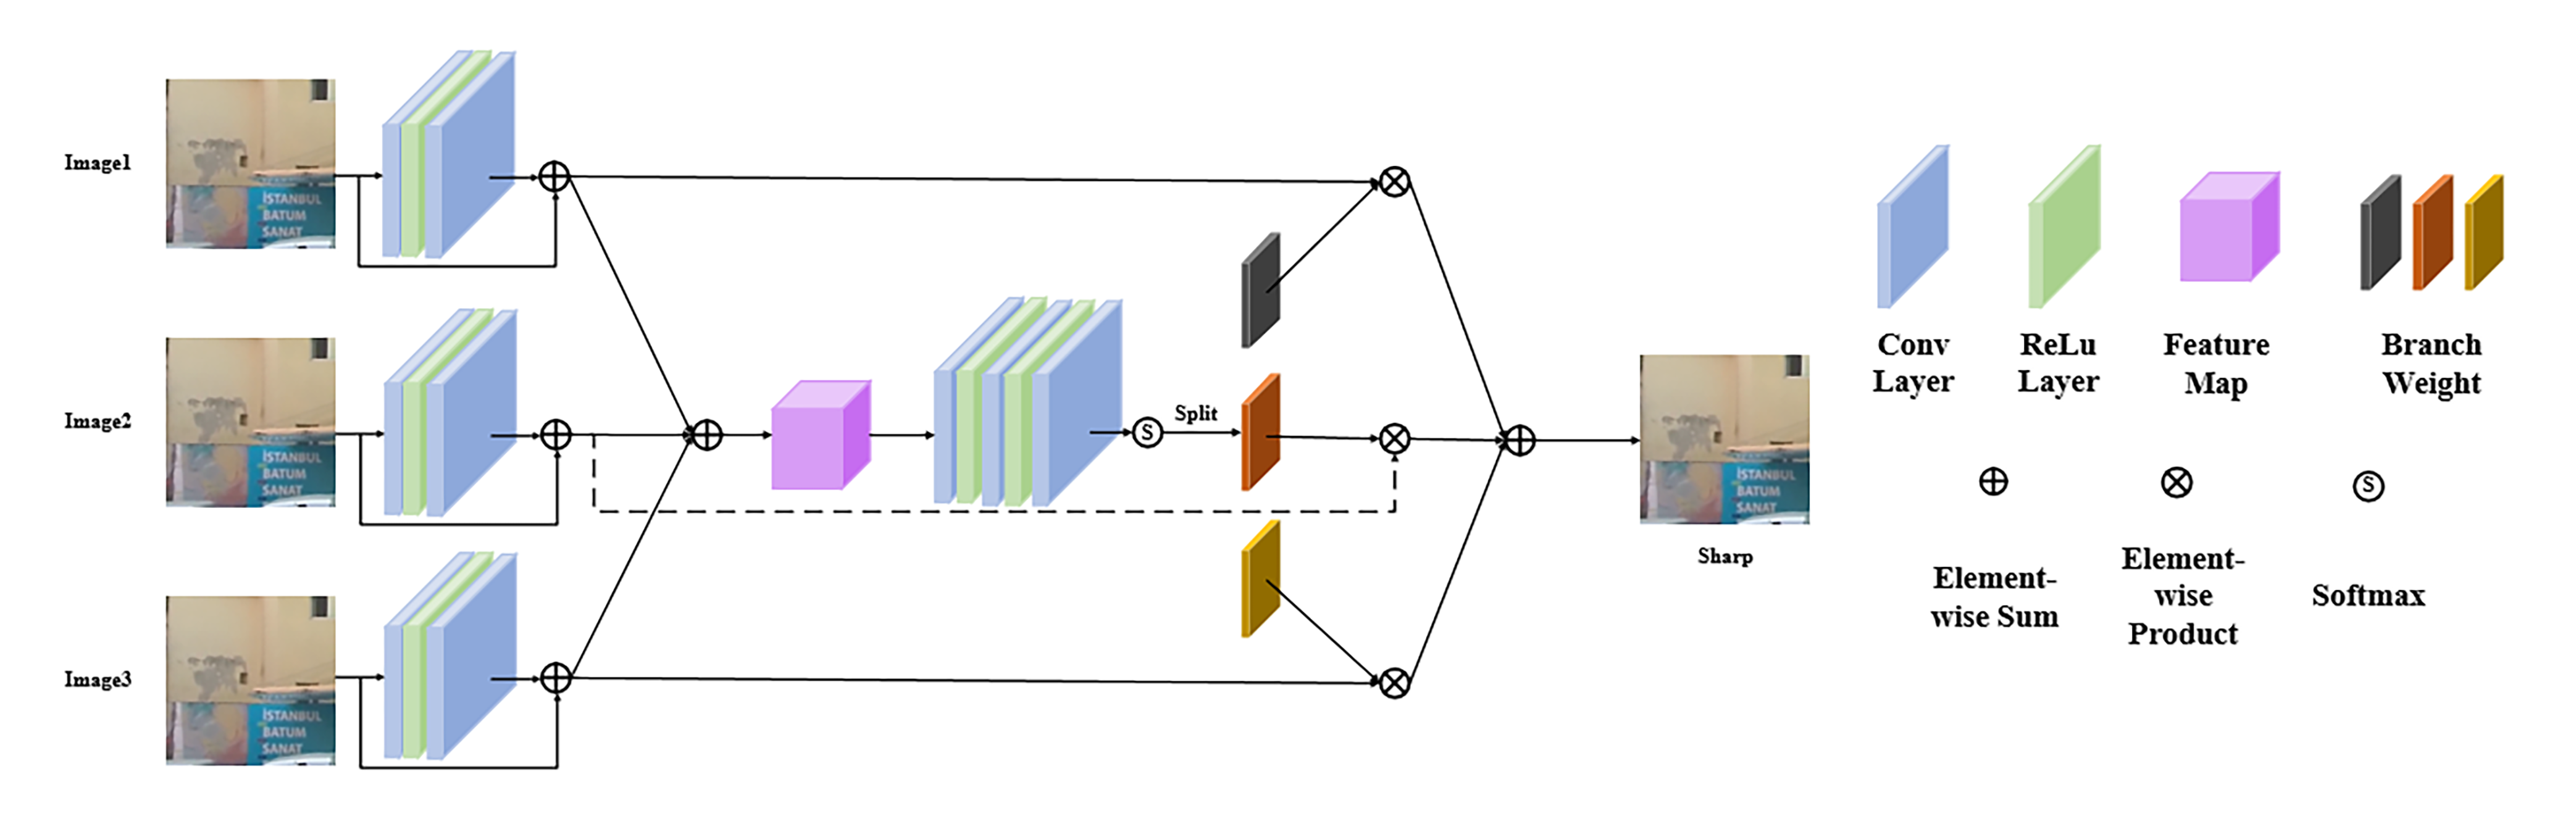
\includegraphics[width=8cm]{images/fig7.png}
\caption{Self-Ensemble Network.}
\label{fig_sim}
\end{figure}
Where $z_{in}^{i,j,c}$ represents the element whose coordinate is (i,j) in the c-th channel of the $z_{in}$. $n$ represents the number of images.

We split $z_{out}$ to get the corresponding coefficient matrix $z^i, i \in (1,n)$ on each branch. Finally, the coefficient matrix $z^i$ is dot-multiplied with its corresponding input image $I_i$ to get the output results of the network.
\subsection{Loss Function}
The loss function of our network mainly includes three parts, i.e. content loss, gradient loss and SSIM loss. And we will describe these parts in detail.
\subsubsection{Content Loss}
We use  content loss to ensure minimizing the pixel-to-pixel differences between the restored image with the ground truth. For content loss, we use the L2 loss as shown in Eqn.(13).
\begin{equation}
	    L_{cont}(I, \hat{I})  =  \frac{1}{H \times W} \sum_{i=0}^{W-1}\sum_{j=0}^{H-1}(I(i,j) - \hat{I}(i, j))^2. \enspace
\end{equation}
Where $I$ represents the sharp image. $\hat{I}$ represents the restored image.
\subsubsection{Gradient Loss}
In order to further improve the proportion of gradient information in the restoration results, we also use gradient loss in the loss functions. It ensures that the gradient of the restored image is consistent with the ground truth. As shown in Eqn.(14), we use L2 loss as the gradient loss.
\begin{equation}
	    L_{grad}(I, \hat{I})  =  \frac{1}{H \times W} \sum_{i=0}^{W-1}\sum_{j=0}^{H-1}(\nabla I(i,j) - \nabla \hat{I}(i, j))^2. \enspace
\end{equation}
Where $\nabla$ represents the Laplacian operator, the proposed gradient extraction operator is designed as Eqn.(15).
\begin{equation}
	    \nabla I = G(F(Ave(I))) * G(F(I)). \enspace
\end{equation}
Where $I$ represents the image. $Ave(\cdot)$ represents the mean filter operation. $F(\cdot)$ represents the Laplacian operator. $G(\cdot)$ stands for normalization operation.
\begin{figure}[h]
%\centeringr
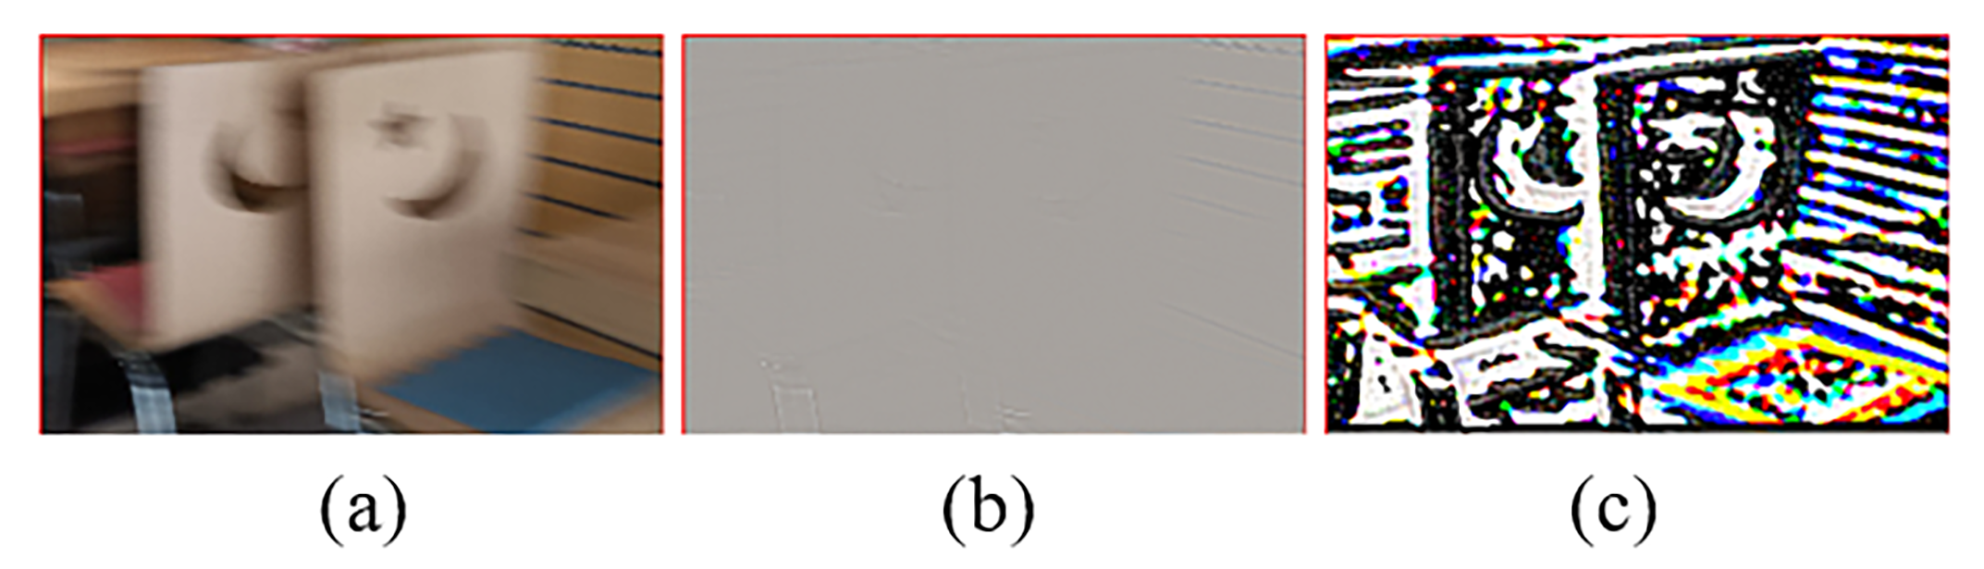
\includegraphics[width=8cm]{images/fig8.png}
\caption{The comparison results of gradient maps which are extracted by different gradient extraction operators. (a) Input image. (b) The result extracted by the Laplacian operator. (c) The gradient map extracted by Eqn.(15).}
\label{fig_sim}
\end{figure}

Using Eqn.(15) for gradient extraction has two advantages. First, it can suppress the influence of noise. Second, it can improve the weight of the gradient information adaptively. As shown in Figure 7, it is proved that the quality of the gradient map can be effectively improved. And many gradients that are invisible previously can be effectively extracted.
\subsubsection{SSIM Loss}
To enable the network to learn more contextually-enriched results, we use the MS-SSIM loss. For the restoration results $R$ and the ground-truth $G$, we calculate the mean $u_R$, $u_G$, the standard deviation $\sigma_R$, $\sigma_G$ and the covariance $\sigma_{RG}$. Then we can calculate MS-SSIM loss according to Eqn.(16).
\begin{equation}
	    L_{ssim} = 1 - \prod^M_{m = 1}(\frac{2u_Ru_G+c_1}{u_R^2+u_G^2+c_1})^{\beta_m}(\frac{2\sigma_{RG}+c_2}{\sigma_R^2+\sigma_G^2+c_2})^{\gamma_m}. \enspace
\end{equation}
Where $m$ represents the different scales. $c_1$ and $c_2$ can maintain the stability during training. $\beta_m$ and $\gamma_m$ represent the relative importance.
\subsubsection{Overall Loss}
We use a combination of content loss, gradient loss, and SSIM loss to construct the overall loss function of the network, as shown in Eqn.(17).
\begin{equation}
	    Loss = \sum_{i=1}^{S}(\alpha L_{cont} + \beta L_{grad} + \gamma L_{ssim}). \enspace
\end{equation}

Where the hyperparameter is $\alpha$=1, $\beta$=0.05, $\gamma$=0.1.

\section{Experiment}
In this section, we first introduce the dataset which is used to verify the effectiveness of our method. Secondly, we describe our experimental configuration. Thirdly, we compare the performance of our method with the existing SOTA methods in dataset and real-world scenarios. Fourthly, we conduct the ablation experiments to verify the effectiveness of the proposed models.
\subsection{Datasets}
\subsubsection{GOPRO}
Nah et al.\cite{3} collected high-frame rate video and then performed motion-blur generation through the multi-frame synthesis. The entire dataset contains 3214 pairs of blur-sharp images, of which 1111 pairs of images are used for test set and 2103 pairs of images are used for training set.

\subsubsection{RealBlur}
Unlike the GOPRO dataset, the RealBlur\cite{25} dataset is collected in the real world and mainly contains two subsets: RealBlur-J is formed with the JPEG images, and RealBlur-R is generated by the RAW images. The dataset contains a total of 4738 pairs of images, of which 980 pairs of images are used for test set and 3758 pairs of images are used for training set.
\subsection{Experiment Settings}
The training process of the network is divided into two stages. In the first stage, we do not train EGN and train the network according to the training strategy in \cite{7}, the patch size of the input is 256$\times$256, the batch size is set to 1, and the network is trained for $6\times10^{6}$ iterations. For data augmentation, we randomly flip the input horizontally or vertically. We train the network using the Adam optimizer with an initial learning rate of $2\times10^{-4}$, which is gradually reduced to $1\times10^{-6}$. In the second training stage, we fix the network parameters which are obtained from the first training stage, and train the EGN separately. The hyperparameters are the same as the first stage. 
\subsection{Comparison with the state-of-the-arts(SOTA) method}
We compare our proposed method with the existing SOTA methods, which include DeblurGAN-v2\cite{18},  MPRNet\cite{7}, MIMONet\cite{9}, etc. We embed EGN into the SOTA method MPRNet. In order to verify the generalization ability of the network, we apply the model to train on the GOPRO dataset and test on the RealBlur dataset. The test results on the GOPRO dataset and the RealBlur dataset are shown in TABLE 1. ‘R-J’ and ‘R-R’ represent ‘RealBlur-J’ and ‘RealBlur-R’, respectively. The best results are shown in bold, and the second best results are shown in the underlined form. It can be seen from TABLE 1 that our method achieves the best results in terms of PSNR and SSIM, which further prove that our network has excellent generalization ability. The visualization results are shown in Figure 8 to Figure 11. Also, we compare the run-time complexity and model complexity with other models, which are tested on the GOPRO dataset. The test results on the GOPRO dataset are shown in TABLE 2. Our run time is longer than MPRNet, because we embed our model into the MPRNet.
\begin{table}[!t]
% increase table row spacing, adjust to taste
\renewcommand{\arraystretch}{1.3}
\caption{The performance comparison of different methods on the GOPRO dataset and the RealBlur dataset.(The model is trained on the GOPRO training set.)}
\label{table1}
\centering
% Some packages, such as MDW tools, offer better commands for making tables
% than the plain LaTeX2e tabular which is used here.
\begin{tabular}{ccc}
\hline\noalign{\smallskip}
Methods & PSNR(GoPro/R-J/R-R) & SSIM(GoPro/R-J/R-R)  \\
\noalign{\smallskip}\hline\noalign{\smallskip}
SRN & 30.26/26.33/33.62 & 0.934/0.856/0.946 \\
DMPHN & 30.45/25.72/33.62 & 0.935/0.844/0.943 \\
DeblurGAN-v2 & 29.55/\underline{26.68}/33.41 & 0.934/0.862/0.936 \\
BANet & 32.44/-/- & 0.957/-/- \\
MIMO-UNet+ & 32.44/26.01/33.65 & 0.957/0.851/0.945 \\
\cite{26} & 31.23/-/- & 0.946/-/- \\
MPRNet & \underline{32.66}/26.51/\underline{33.91} & \underline{0.959}/\underline{0.865}/\underline{0.949} \\
Ours & \bf{33.00/26.96/34.30} & \bf{0.961/0.877/0.952} \\
\noalign{\smallskip}\hline
\end{tabular}
\end{table}

\begin{table}[!t]
% increase table row spacing, adjust to taste
\renewcommand{\arraystretch}{1.3}
\caption{The  run-time complexity comparison of different methods on the GOPRO dataset.(The model is trained on the GOPRO training set.)}
\label{table2}
\centering
% Some packages, such as MDW tools, offer better commands for making tables
% than the plain LaTeX2e tabular which is used here.
\begin{tabular}{ccc}
\hline\noalign{\smallskip}
Methods & Run Time(s) & Model Size(MB) \\
\noalign{\smallskip}\hline\noalign{\smallskip}
DMPHN & 0.135 & 29.01 \\
MPRNet & 0.217 & 20.13 \\
MIMO-UNet+  & 0.028 & 16.11 \\
DeblurGAN-v2 & 0.115 & 28.27 \\
\cite{26} & 0.790 & 26.34 \\
Ours & 0.231 & 26.60 \\
\noalign{\smallskip}\hline
\end{tabular}
\end{table}


Finally, we use mobile phone to capture the images in real indoor and outdoor scenes. We also compare the processing results with the other methods. Since the captured images do not have the corresponding sharp images, we only show qualitative comparisons. As shown in Figure 12, our images are much sharper and contain much more gradient information.

\subsection{Ablation Study}
In this section, we further analyze the effectiveness of our proposed network through ablation study, mainly from the following aspects: 1) the input of EGN; 2) the attention mechanism in EGN; 3) effectiveness of EGN; 4) effectiveness of Gradient Loss.
\subsubsection{The input of EGN}
Inspired by YOLOR\cite{27}, we design various inputs for EGN, i. e. random initialization with a mean value of 0 or 1, which is added or multiplied to the network. It is tested on the GOPRO dataset, and the obtained results are shown in TABLE 3. In TABLE 3, the ‘add’ and ‘mul’ mean to fuse with the feature map in the form of addition and multiplication, respectively. Random(a,b) means a normal distribution with mean ‘a’ and standard deviation ‘b’.

\begin{table}[!t]
% increase table row spacing, adjust to taste
\renewcommand{\arraystretch}{1.3}
\caption{Comparative experimental results on the GOPRO dataset when using different inputs for EGN.}
\label{table3}
\centering
% Some packages, such as MDW tools, offer better commands for making tables
% than the plain LaTeX2e tabular which is used here.
\begin{tabular}{ccc}
\hline\noalign{\smallskip}
Input & PSNR(w A-w/o A) & SSIM(w A-w/o A)  \\
\noalign{\smallskip}\hline\noalign{\smallskip}
add+random(0,0.02) & 32.9088/32.9081 & 0.9609/0.9608 \\
add+random(0,0.2) & 32.9088/32.9080 & 0.9609/0.9609 \\
mul+random(1,0.02) & 32.9080/32.9068 & 0.9608/0.9608 \\
Ours & \bf{32.9250/32.9154} & \bf{0.9610/0.9609} \\
\noalign{\smallskip}\hline
\end{tabular}
\end{table}

It can be seen from TABLE 3 that our network has good adaptability to different forms of input, and can get good results on the GOPRO dataset. In TABLE 3, ‘w A’ and ‘w/o A’ represent ‘with Attention’ and ‘without Attention’, respectively. It is proved that our network is very robust to the different inputs. And EGN can adaptively learn more weights which are beneficial to image deblurring.

\subsubsection{The Attention Module in EGN}
In order to verify the effectiveness of the attention mechanism in EGN. We redesign EGN and make it only contain continuous convolution layers. The experimental results tested on the GOPRO dataset are shown in TABLE 3.

It can be seen from TABLE 3 that a variety of network structures can get good results, but the best results are obtained by using the attention module. The effectiveness of the attention module is confirmed.

\begin{table}[!t]
% increase table row spacing, adjust to taste
\renewcommand{\arraystretch}{1.3}
\caption{The comparative experimental results of the network with and without EGN on the GOPRO dataset.}
\label{table4}
\centering
% Some packages, such as MDW tools, offer better commands for making tables
% than the plain LaTeX2e tabular which is used here.
\begin{tabular}{ccc}
\hline\noalign{\smallskip}
 & PSNR & SSIM \\
\noalign{\smallskip}\hline\noalign{\smallskip}
w/o EGN & 32.52 & 0.958 \\
w EGN & \bf{32.92} & \bf{0.961} \\
\noalign{\smallskip}\hline
\end{tabular}
\end{table}

\begin{table}[!t]
% increase table row spacing, adjust to taste
\renewcommand{\arraystretch}{1.3}
\caption{The HSIC comparison of the results on the GOPRO dataset with and without EGN.}
\label{table5}
\centering
% Some packages, such as MDW tools, offer better commands for making tables
% than the plain LaTeX2e tabular which is used here.
\begin{tabular}{ccc}
\hline\noalign{\smallskip}
 & blur & sharp  \\
\noalign{\smallskip}\hline\noalign{\smallskip}
w/o EGN & 1 & 1.6838 \\
w EGN & 1 & \bf{1.8134} \\
\noalign{\smallskip}\hline
\end{tabular}
\end{table}


\begin{figure}
        \center
        \scriptsize
        \begin{tabular}{ccc}
                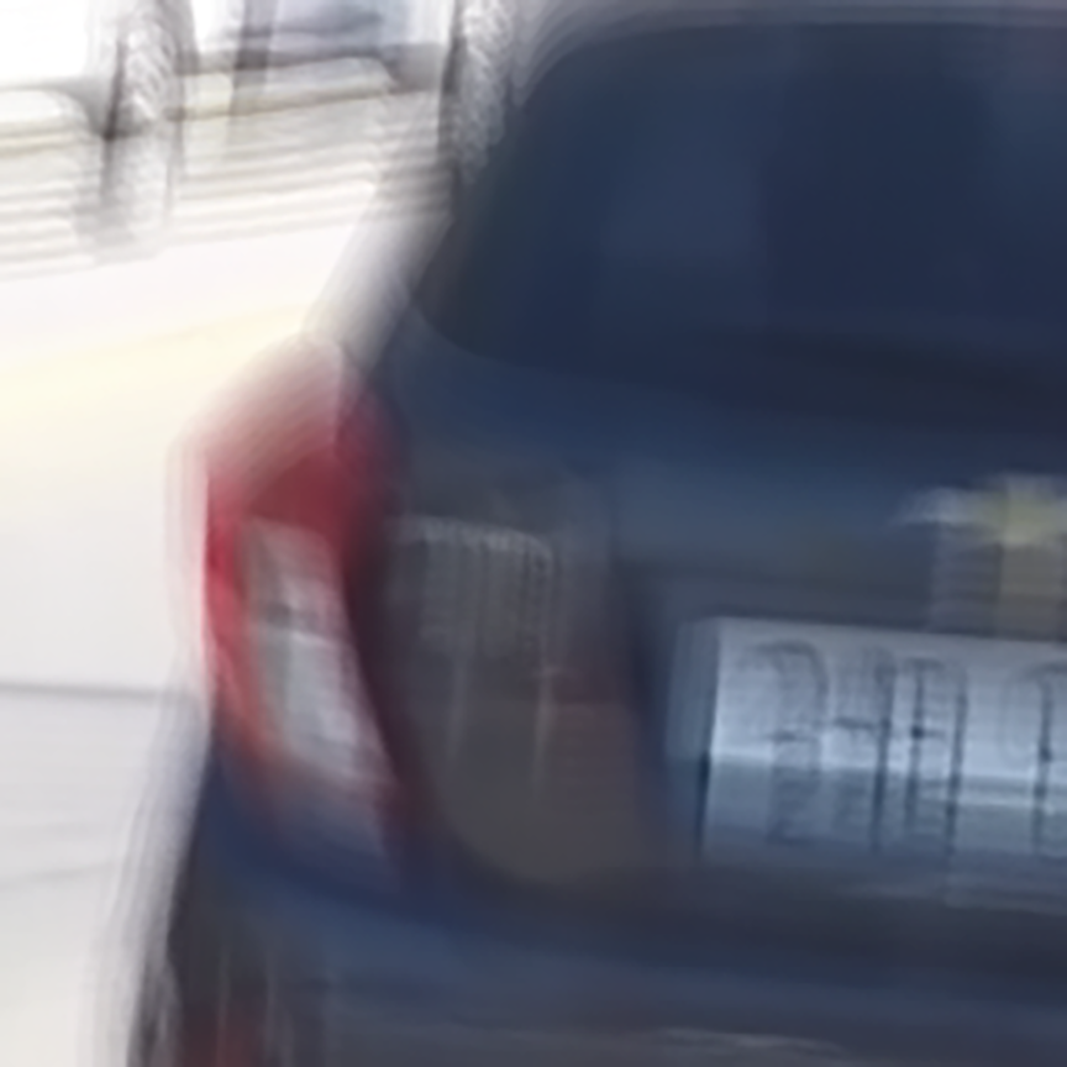
\includegraphics[width=1.3cm,height=1.3cm]{./gopro2/GOPR0854_11_00_000005_2_1.png} &    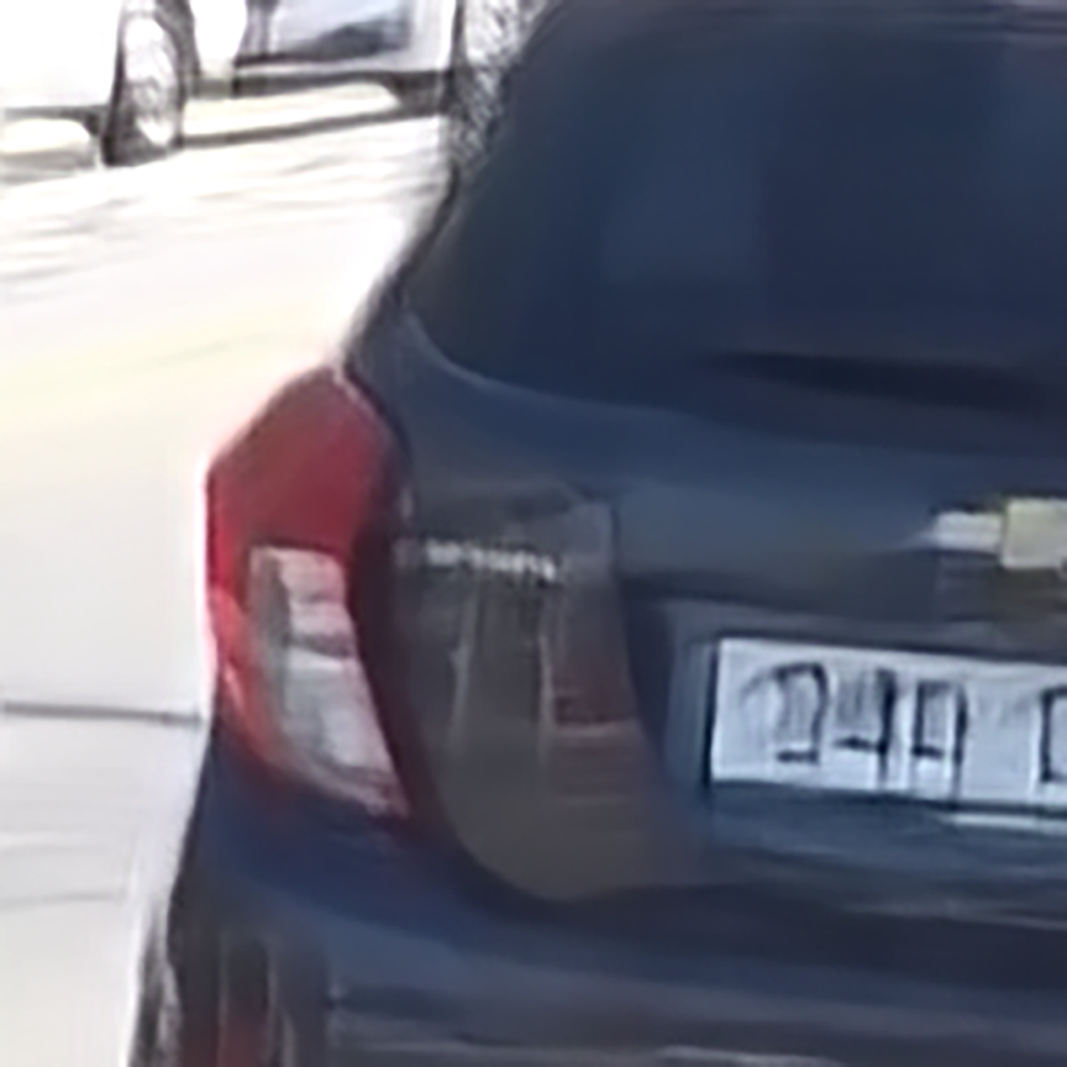
\includegraphics[width=1.3cm,height=1.3cm]{./gopro2/GOPR0854_11_00_000005_D-GAN2_2_1.png} &    
                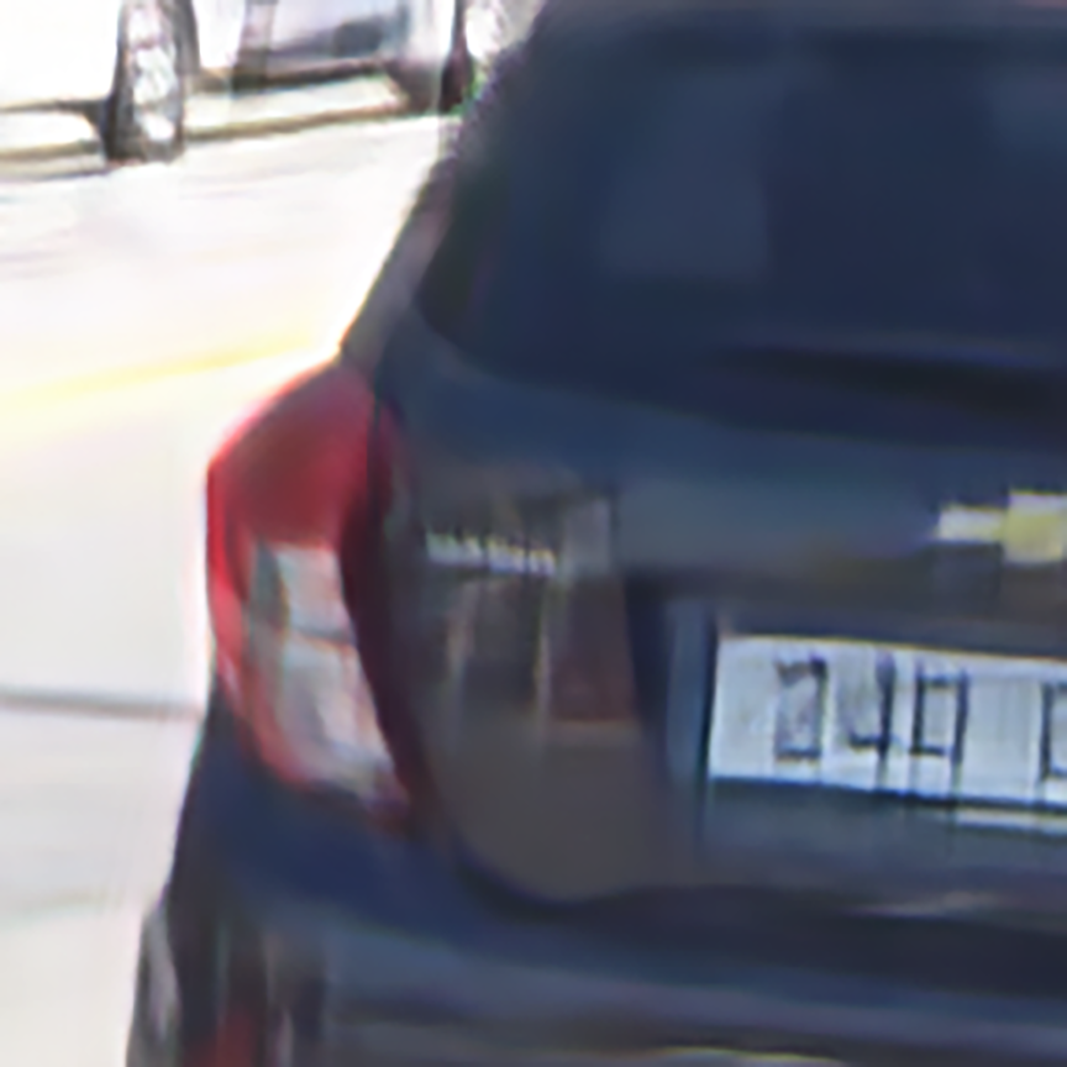
\includegraphics[width=1.3cm,height=1.3cm]{./gopro2/GOPR0854_11_00_000005_SRN_2_1.png}       \\
                blur & DeblurGAN-v2 & SRN \\
                
                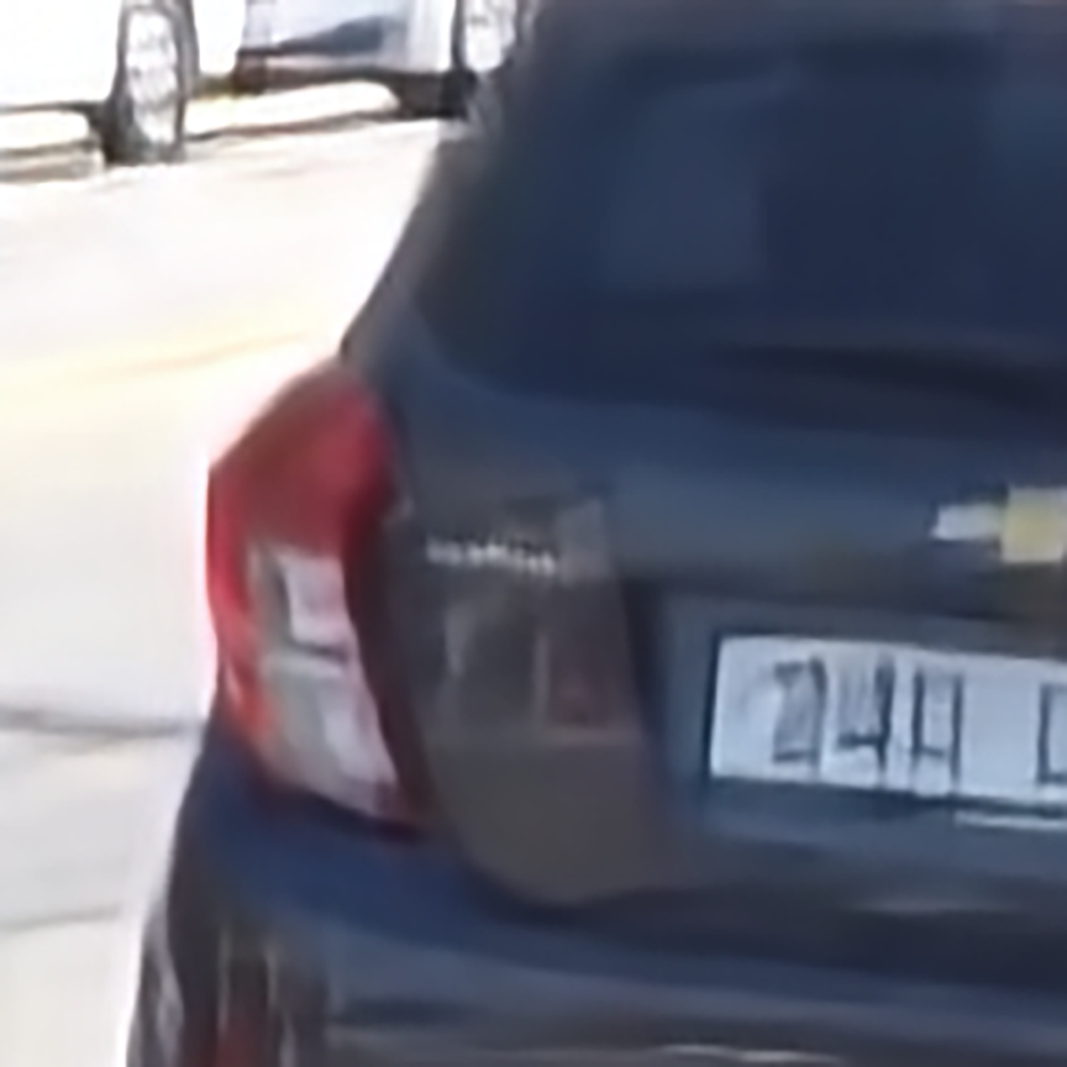
\includegraphics[width=1.3cm,height=1.3cm]{./gopro2/GOPR0854_11_00_000005_DMPHN_2_1.png} &    
                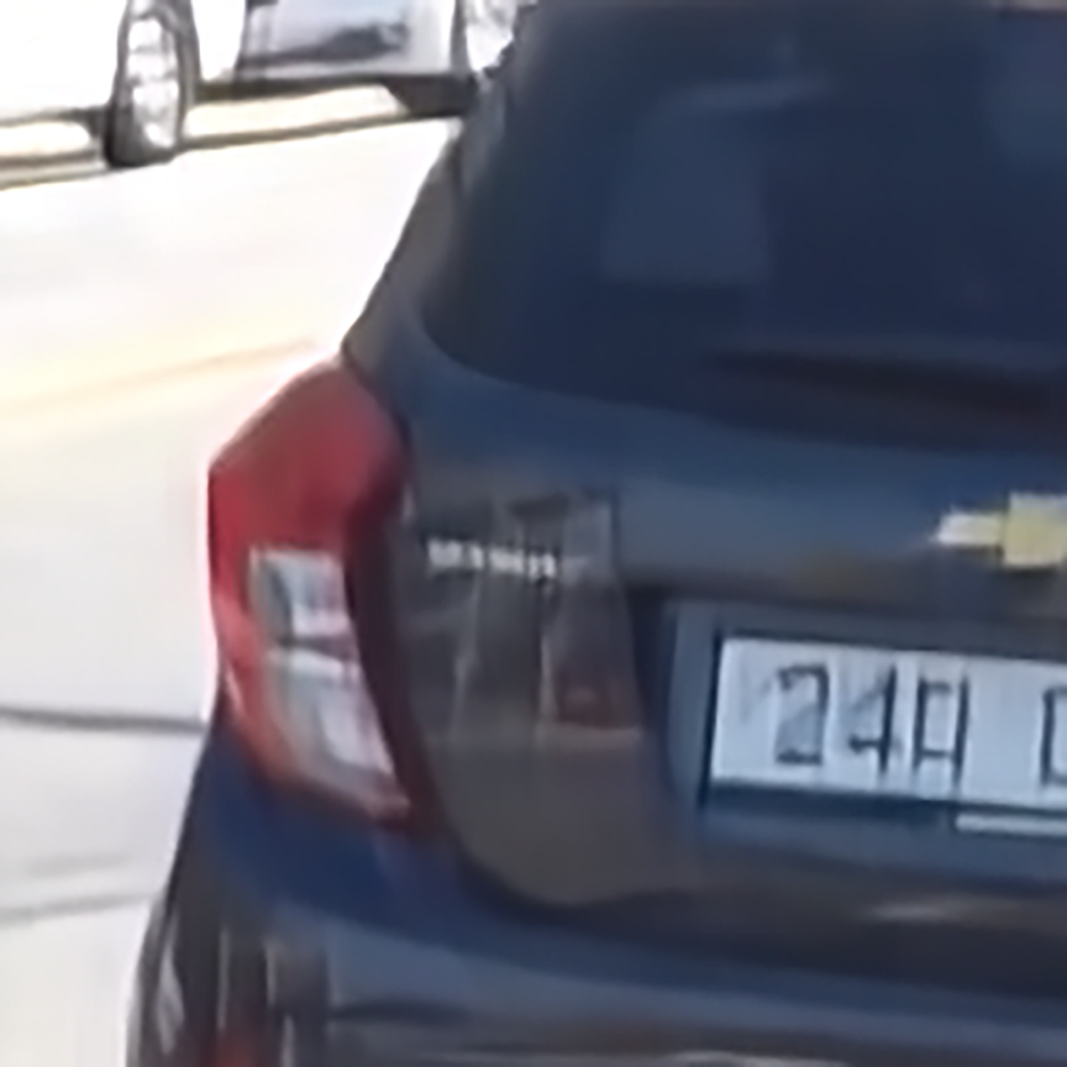
\includegraphics[width=1.3cm,height=1.3cm]{./gopro2/GOPR0854_11_00_000005_MIMO_2_1.png} &    
                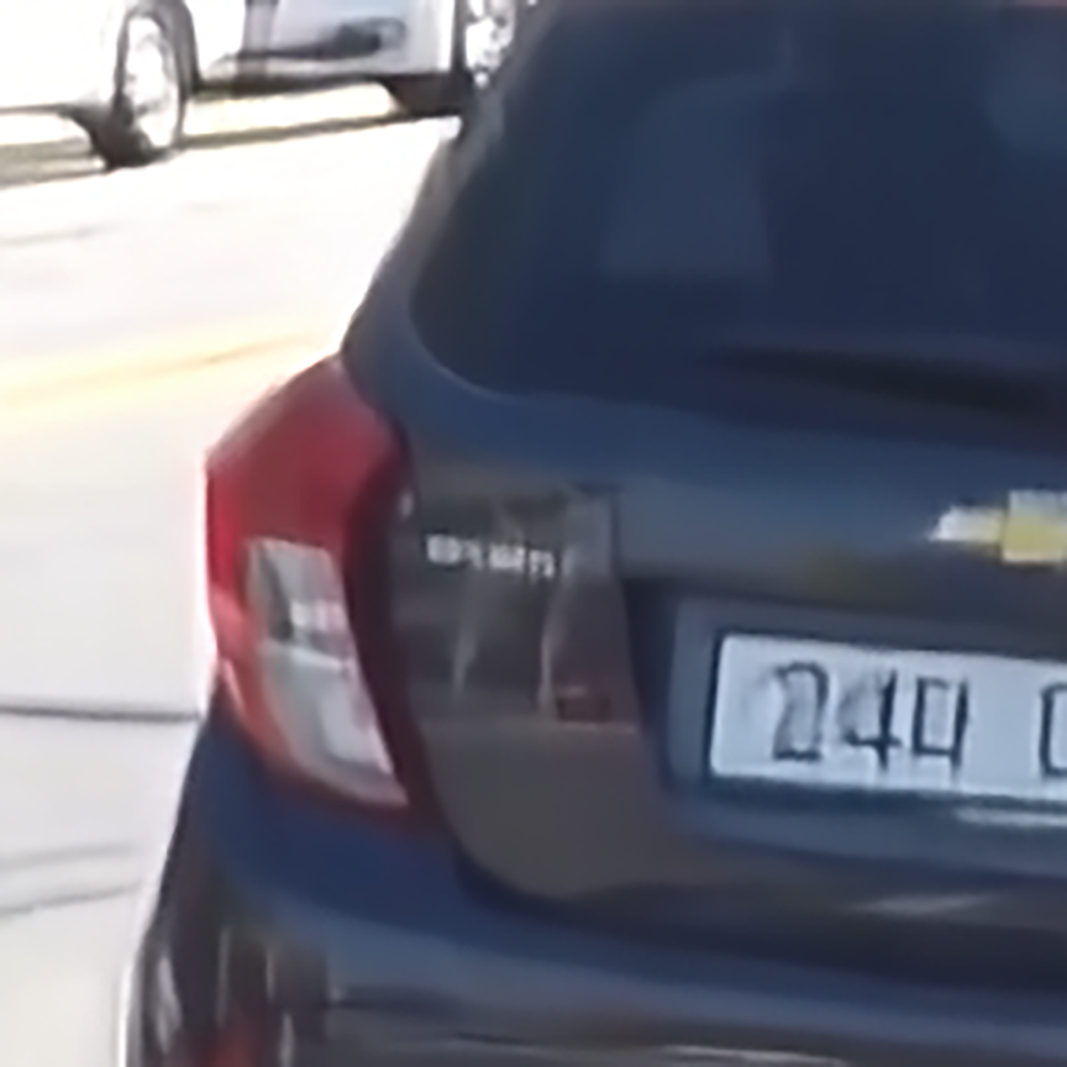
\includegraphics[width=1.3cm,height=1.3cm]{./gopro2/GOPR0854_11_00_000005_MPR_2_1.png}       \\
                DMPHN & MIMO-UNet+ & MPRNet \\
                

                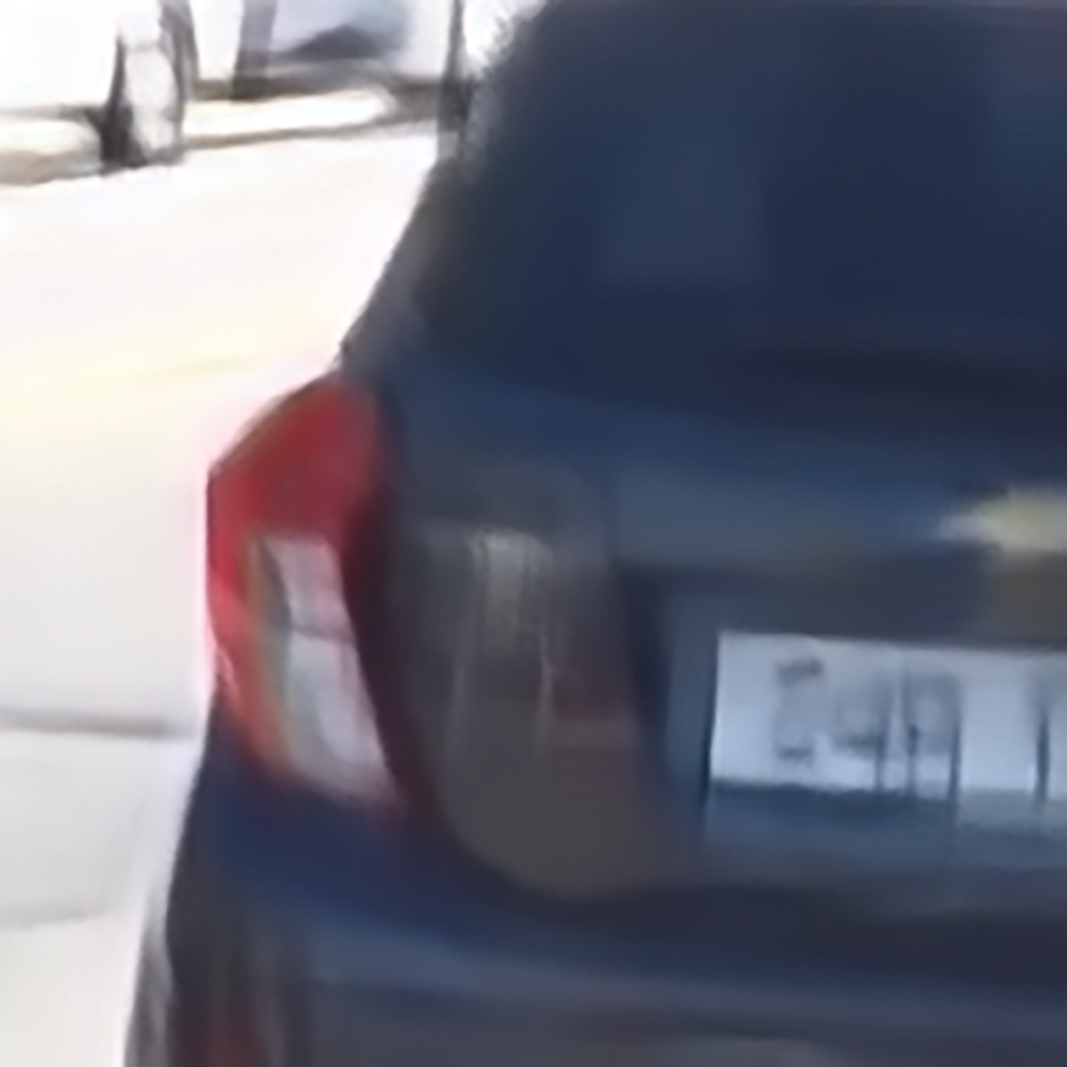
\includegraphics[width=1.3cm,height=1.3cm]{./gopro2/GOPR0854_11_00_000005_2_1_AD.png} &
                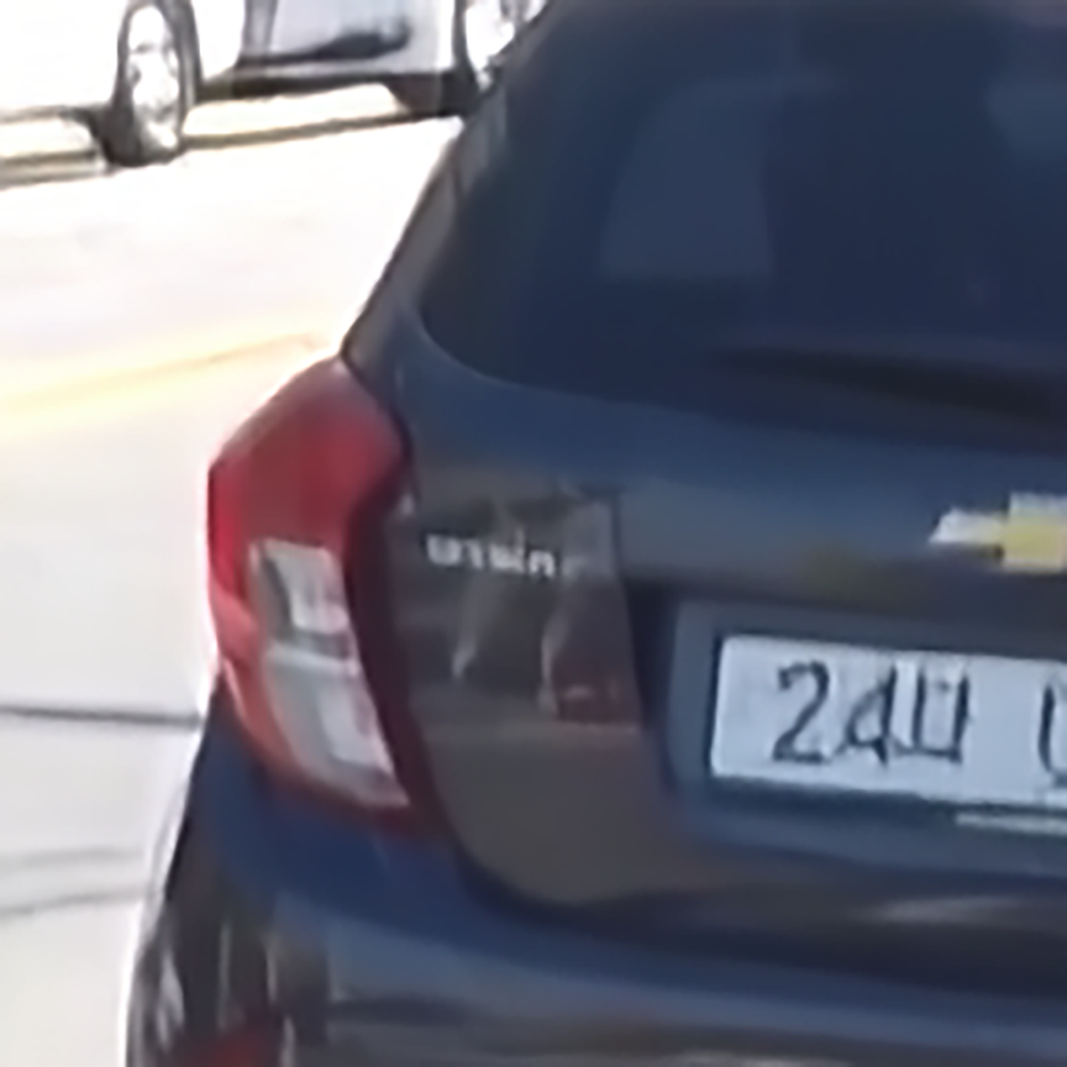
\includegraphics[width=1.3cm,height=1.3cm]{./gopro2/GOPR0854_11_00_000005_ours_2_1.png} &    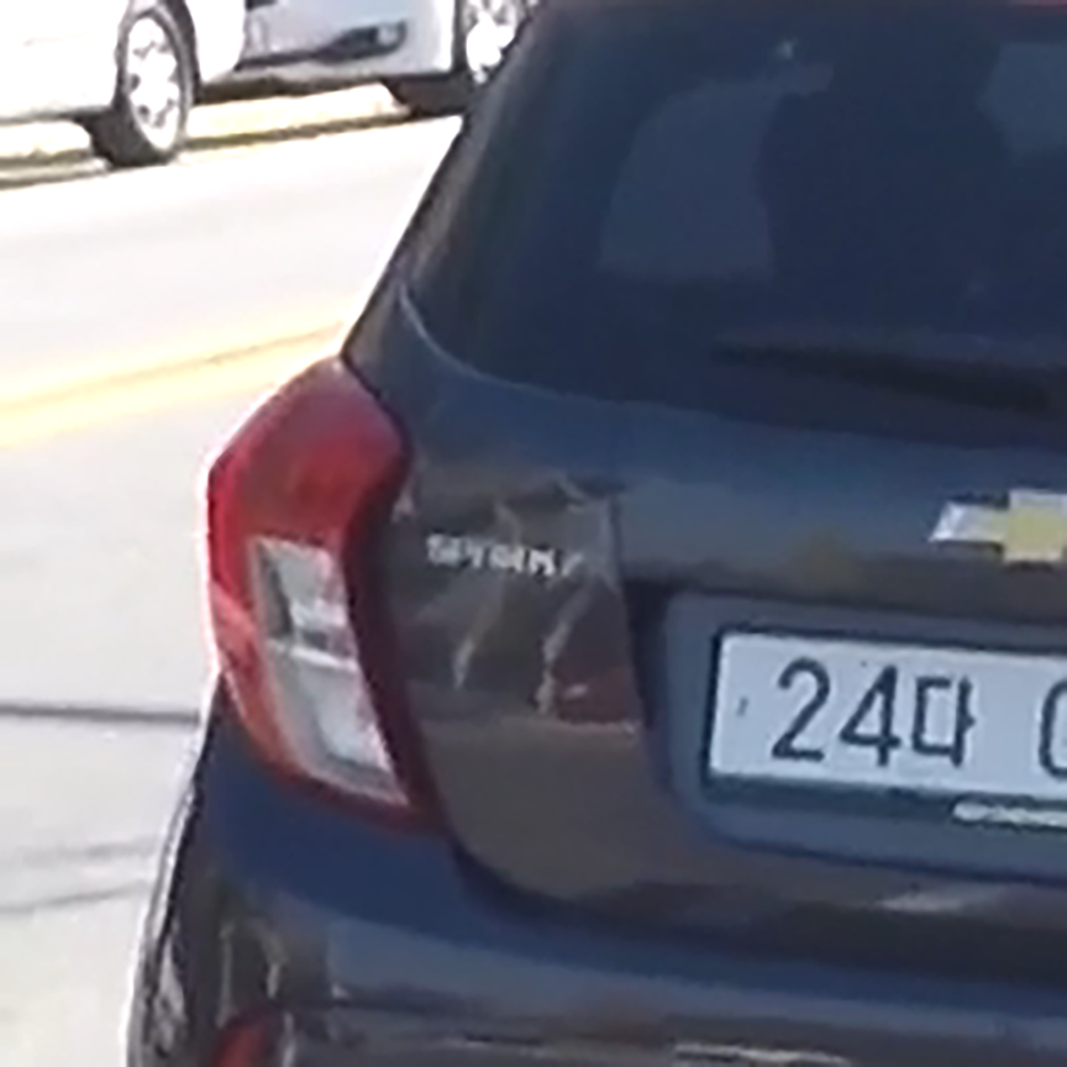
\includegraphics[width=1.3cm,height=1.3cm]{./gopro2/GOPR0854_11_00_000005_2_1_sharp.png}    \\
                \textcolor{black}{\cite{26}} & Ours & sharp \\
                
        \end{tabular}
        \caption{The comparison of the results between the SOTA  methods with our proposed method on the GOPRO dataset.}
        \label{figure8}
        \vspace{-0.5em}
\end{figure}

\begin{figure}
        \center
        \scriptsize
        \begin{tabular}{ccc}
                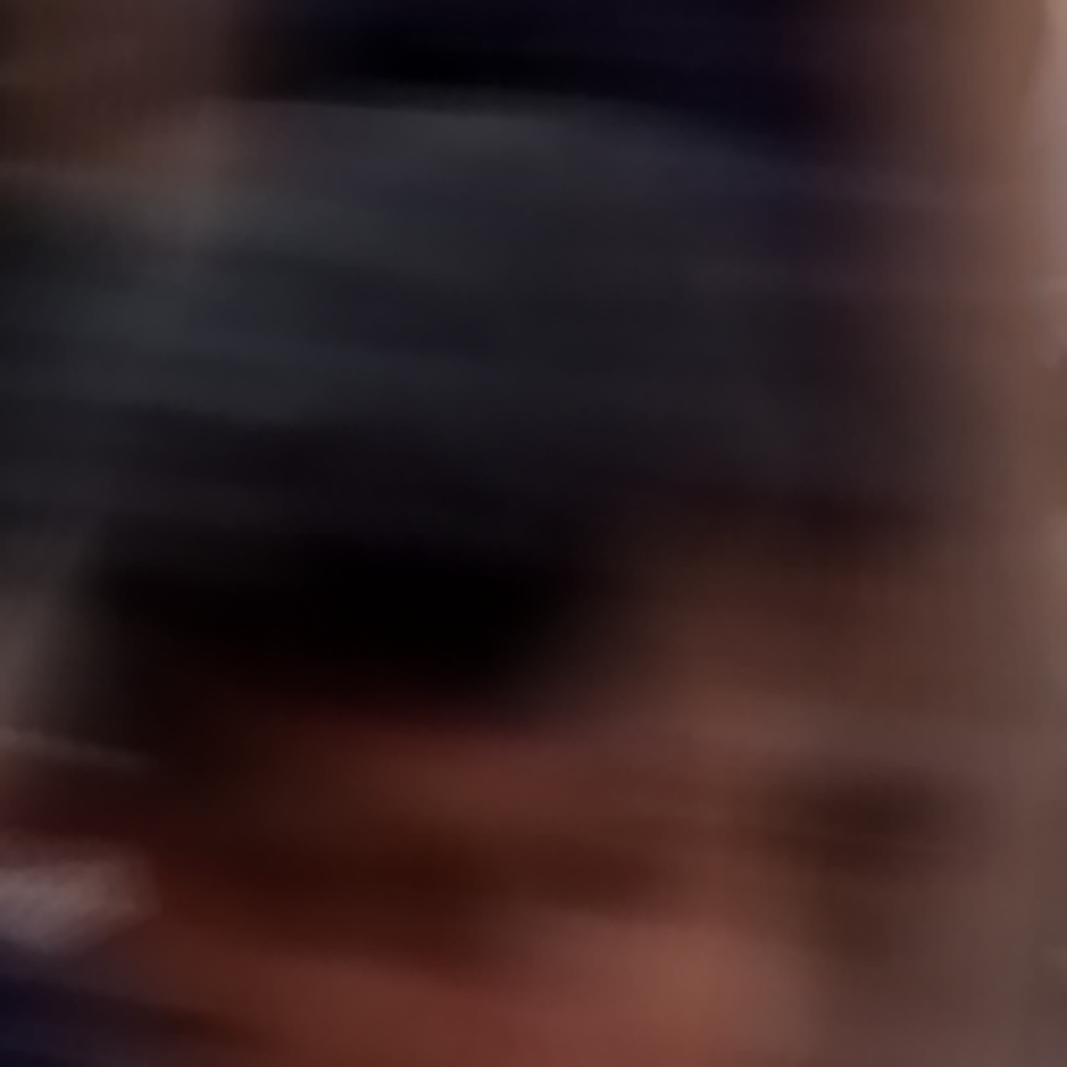
\includegraphics[width=1.3cm,height=1.3cm]{./gopro1/GOPR0384_11_05_004004_3_5.png} &    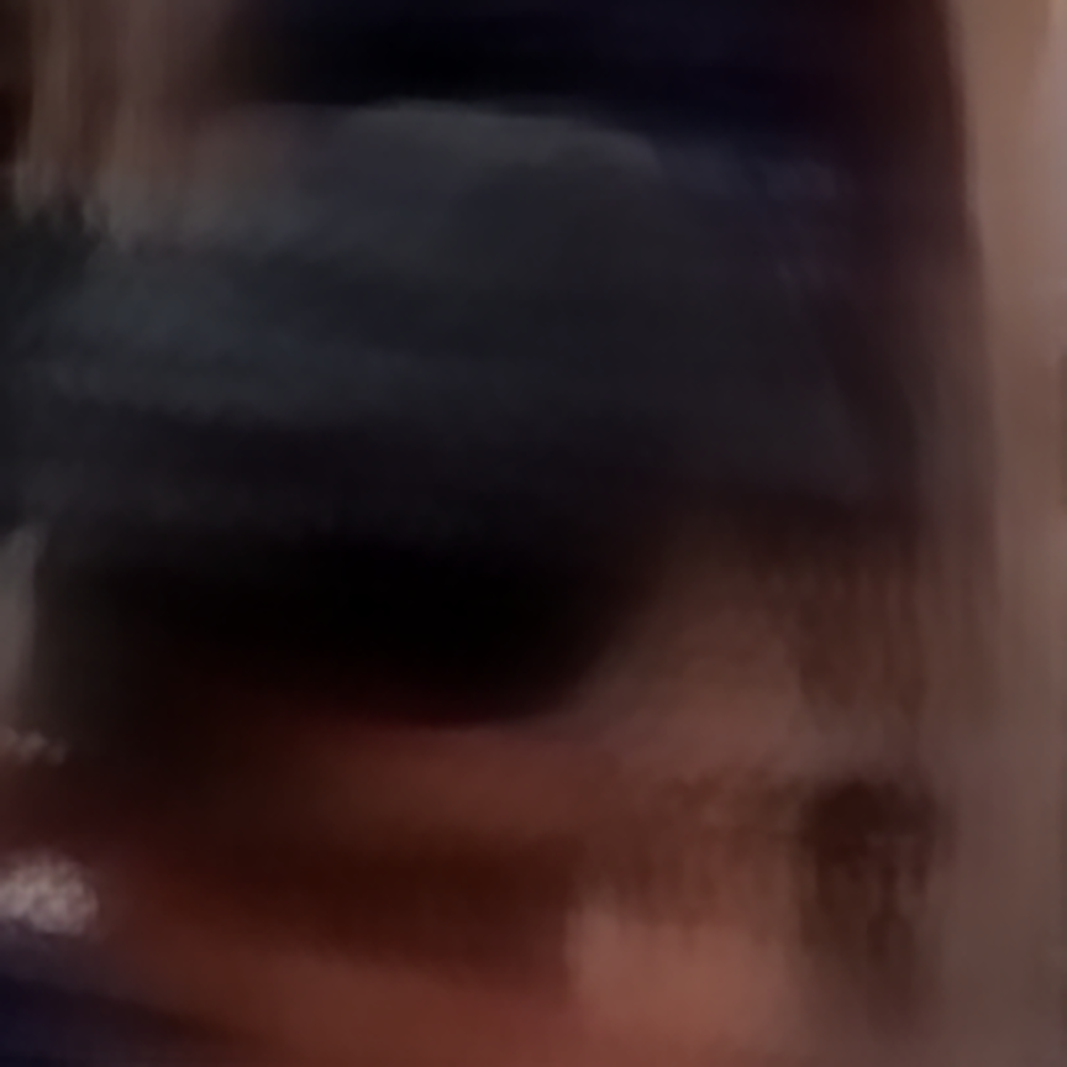
\includegraphics[width=1.3cm,height=1.3cm]{./gopro1/GOPR0384_11_05_004004_D-GAN2_3_5.png} &    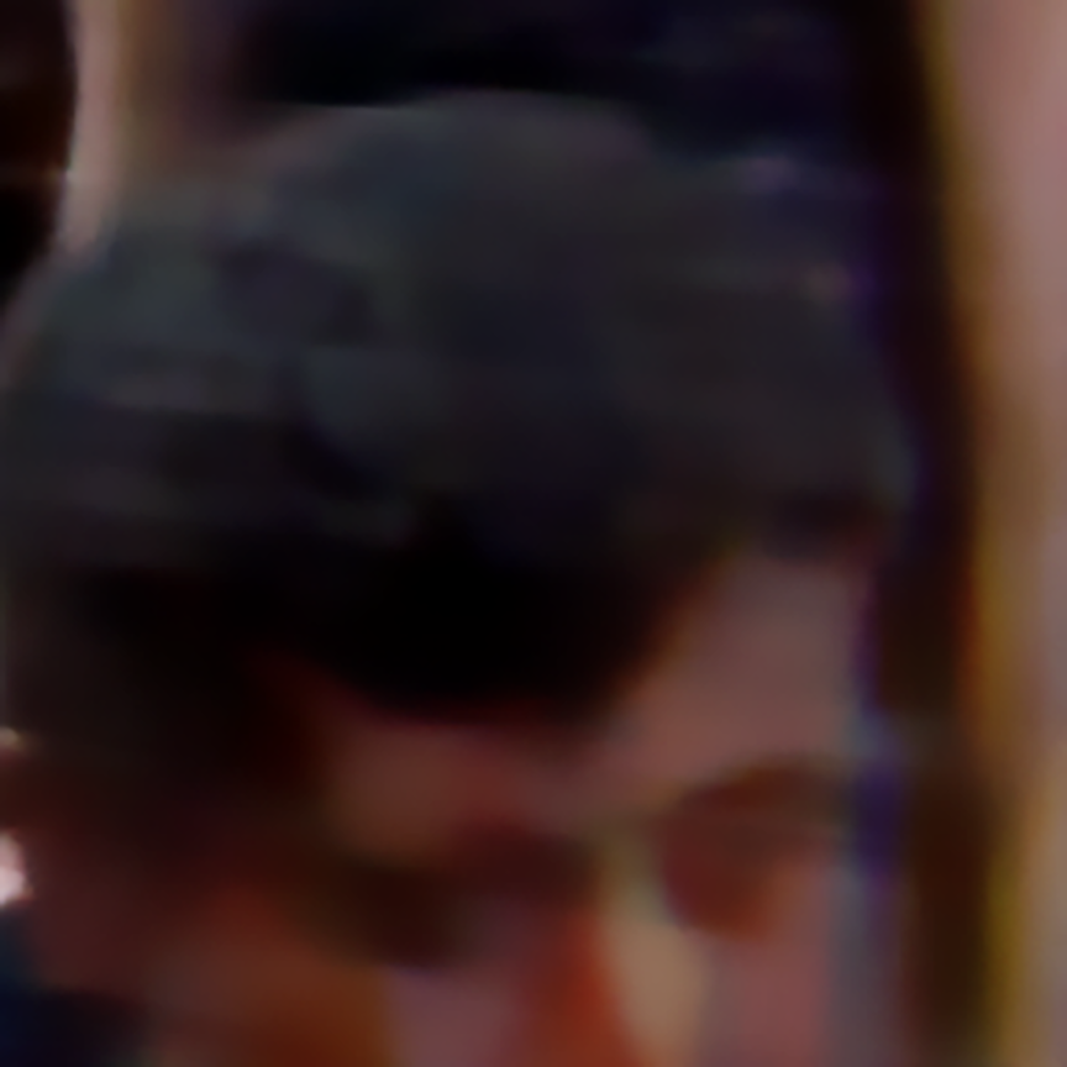
\includegraphics[width=1.3cm,height=1.3cm]{./gopro1/GOPR0384_11_05_004004_SRN_3_5.png}       \\
                \textcolor{black}{blur} & \textcolor{black}{DeblurGAN-v2} & \textcolor{black}{SRN} \\
                
                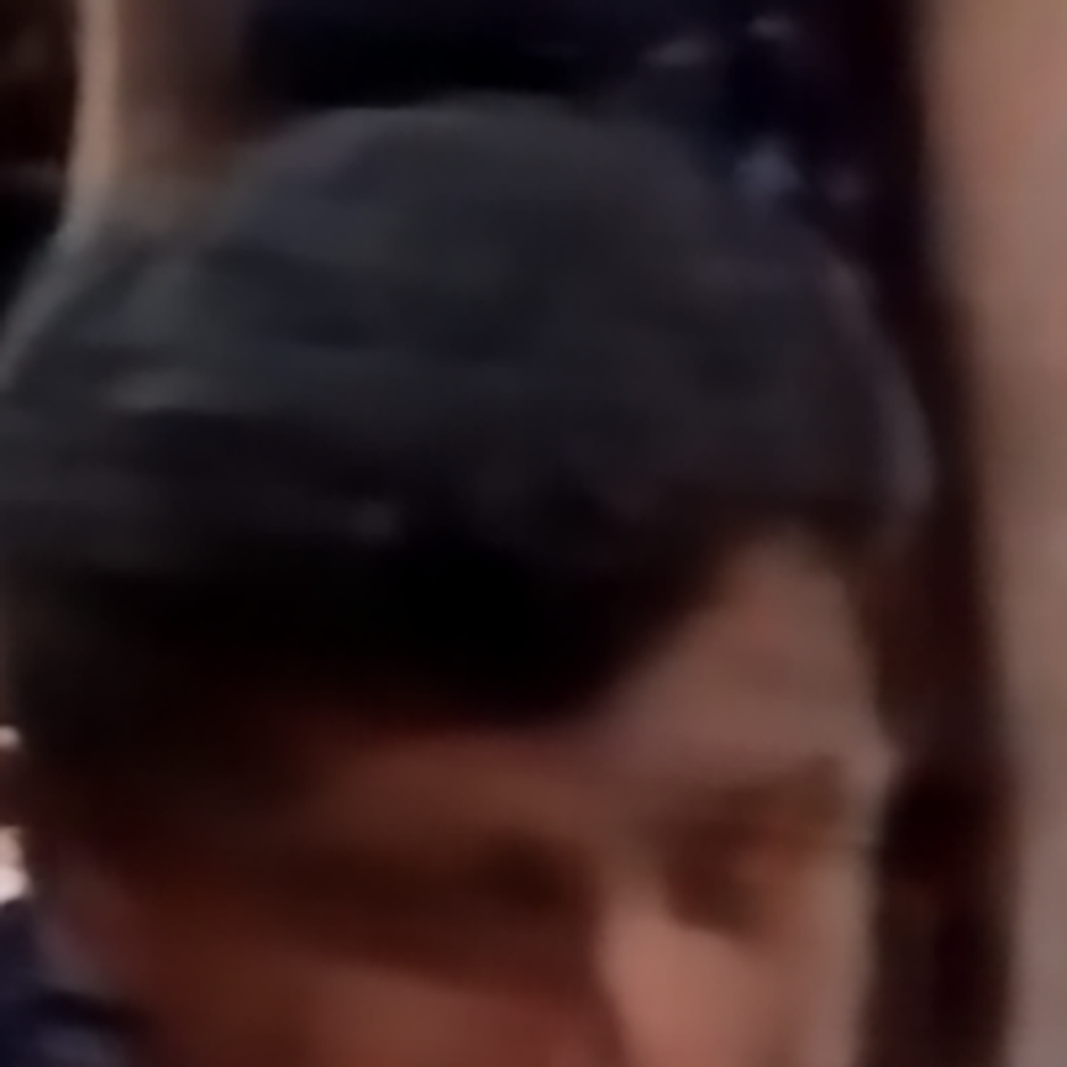
\includegraphics[width=1.3cm,height=1.3cm]{./gopro1/GOPR0384_11_05_004004_DMPHN_3_5.png} &    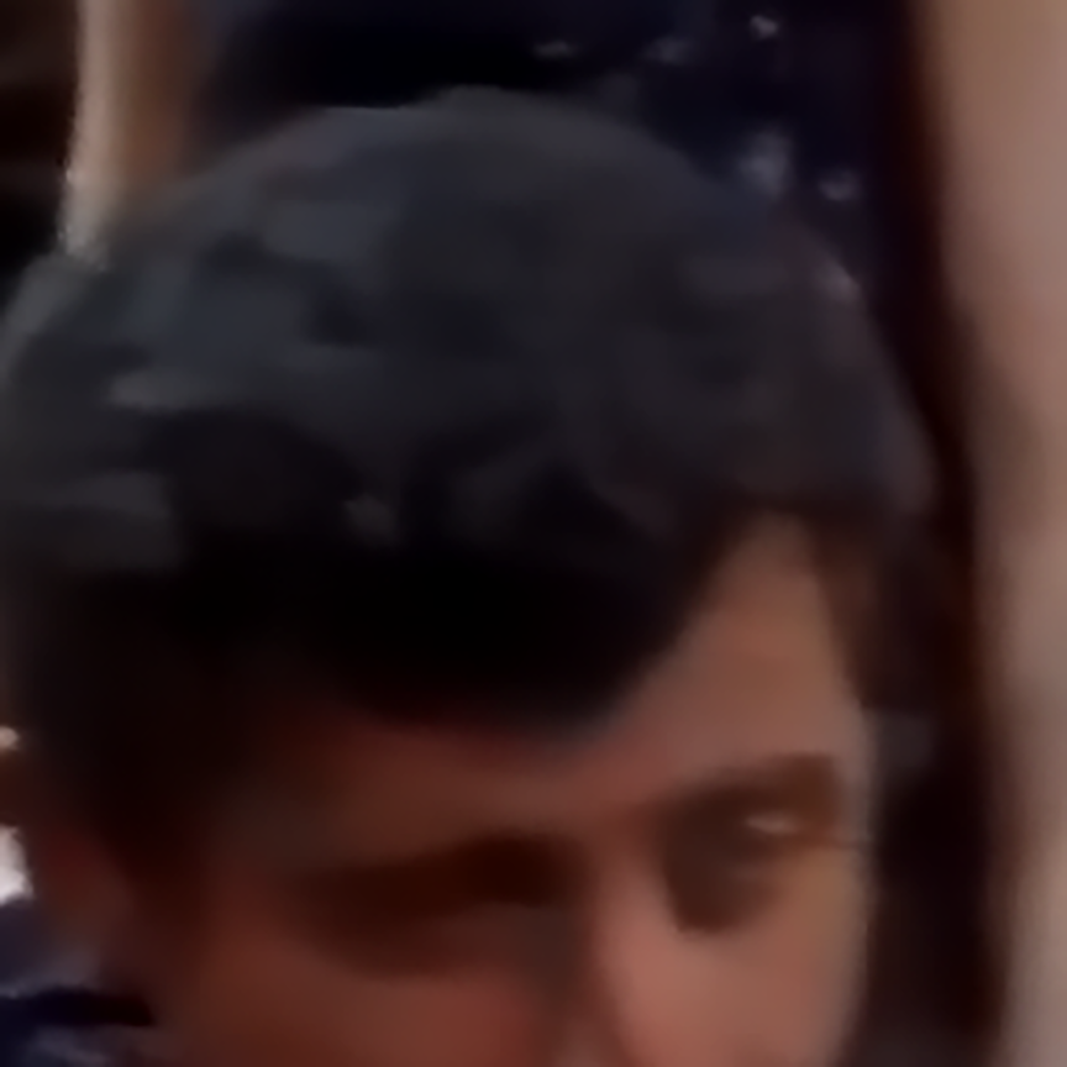
\includegraphics[width=1.3cm,height=1.3cm]{./gopro1/GOPR0384_11_05_004004_MIMO_3_5.png} &    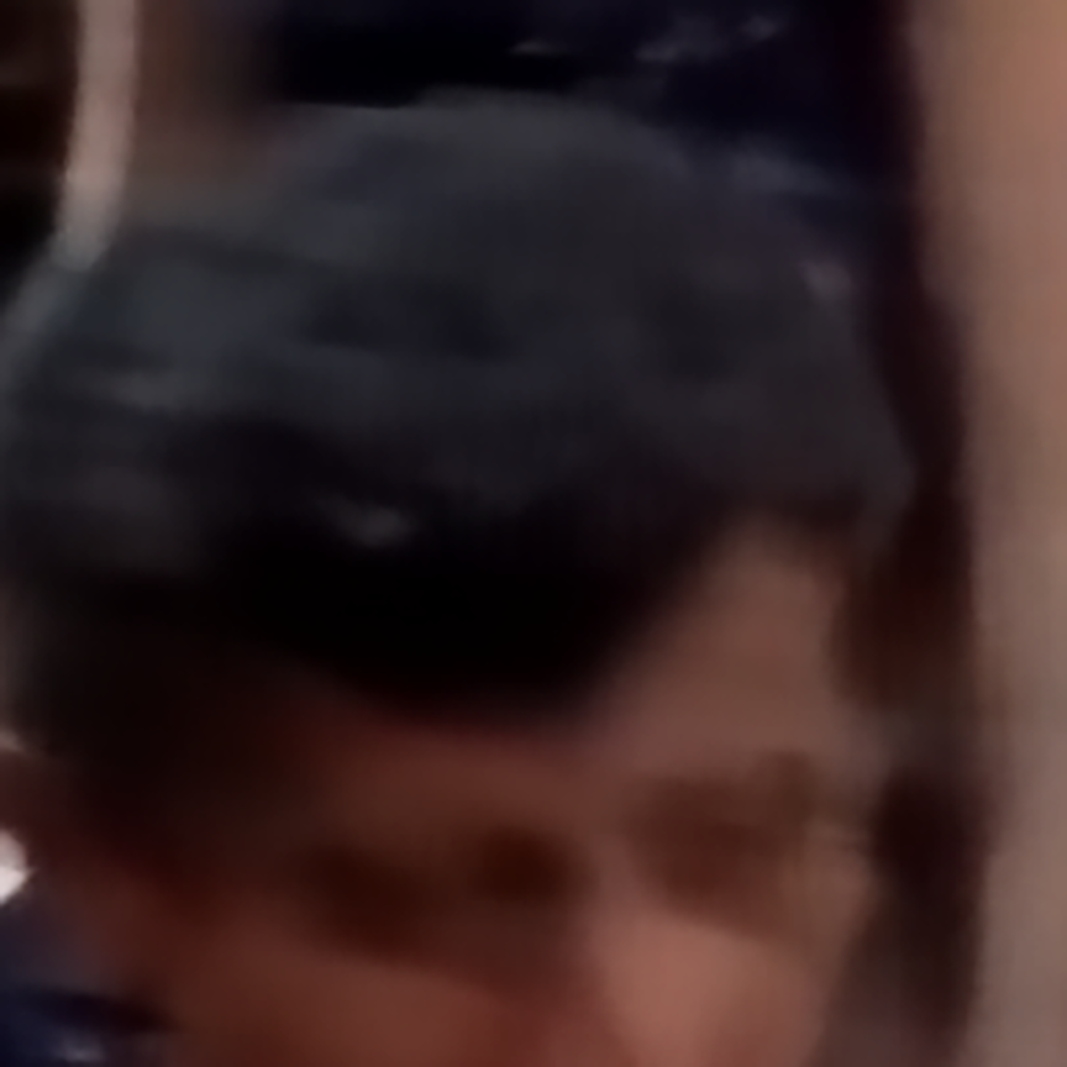
\includegraphics[width=1.3cm,height=1.3cm]{./gopro1/GOPR0384_11_05_004004_MPR_3_5.png}       \\
                \textcolor{black}{DMPHN} & \textcolor{black}{MIMO-UNet+} & \textcolor{black}{MPRNet} \\

                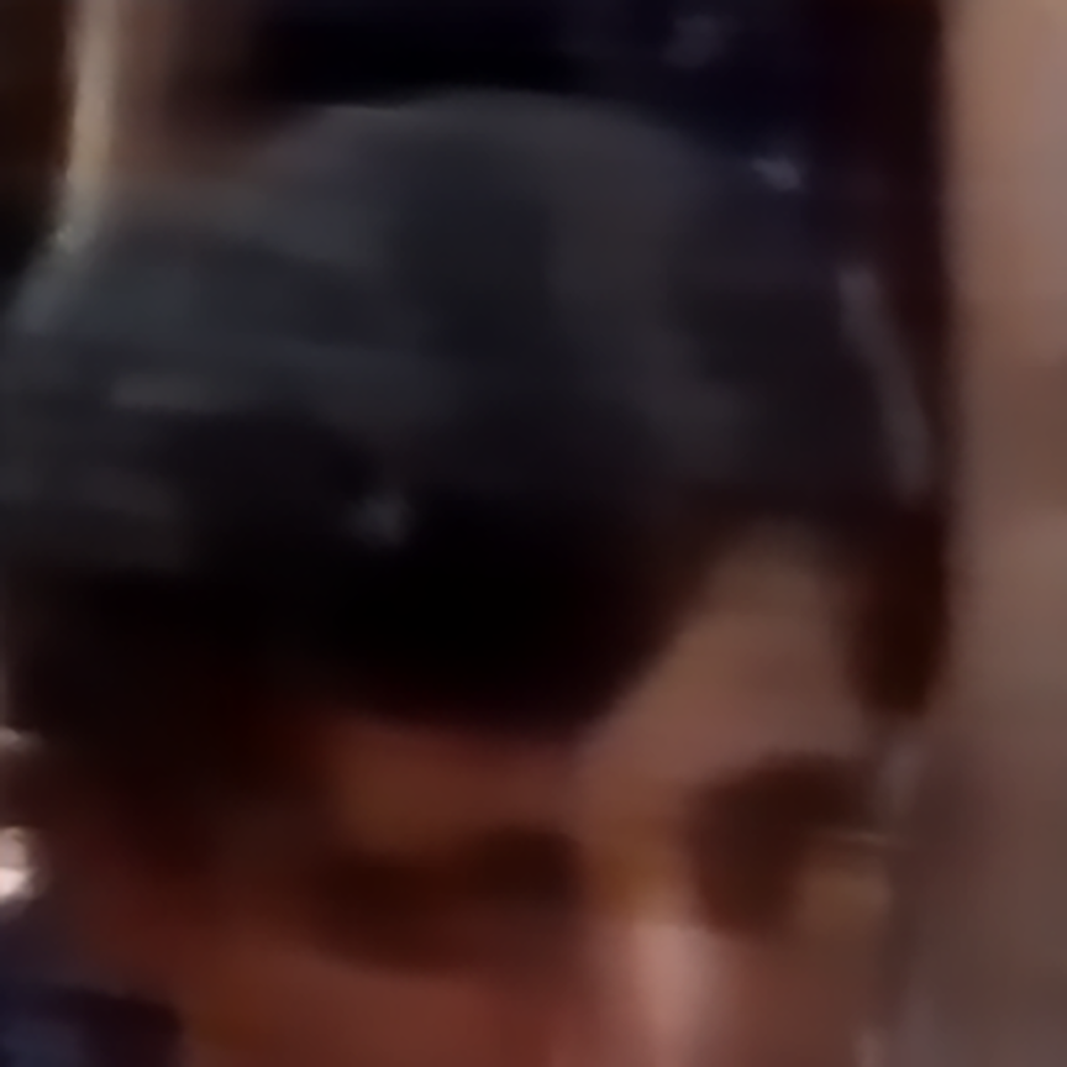
\includegraphics[width=1.3cm,height=1.3cm]{./gopro1/GOPR0384_11_05_004004_3_5_AD.png} & 
                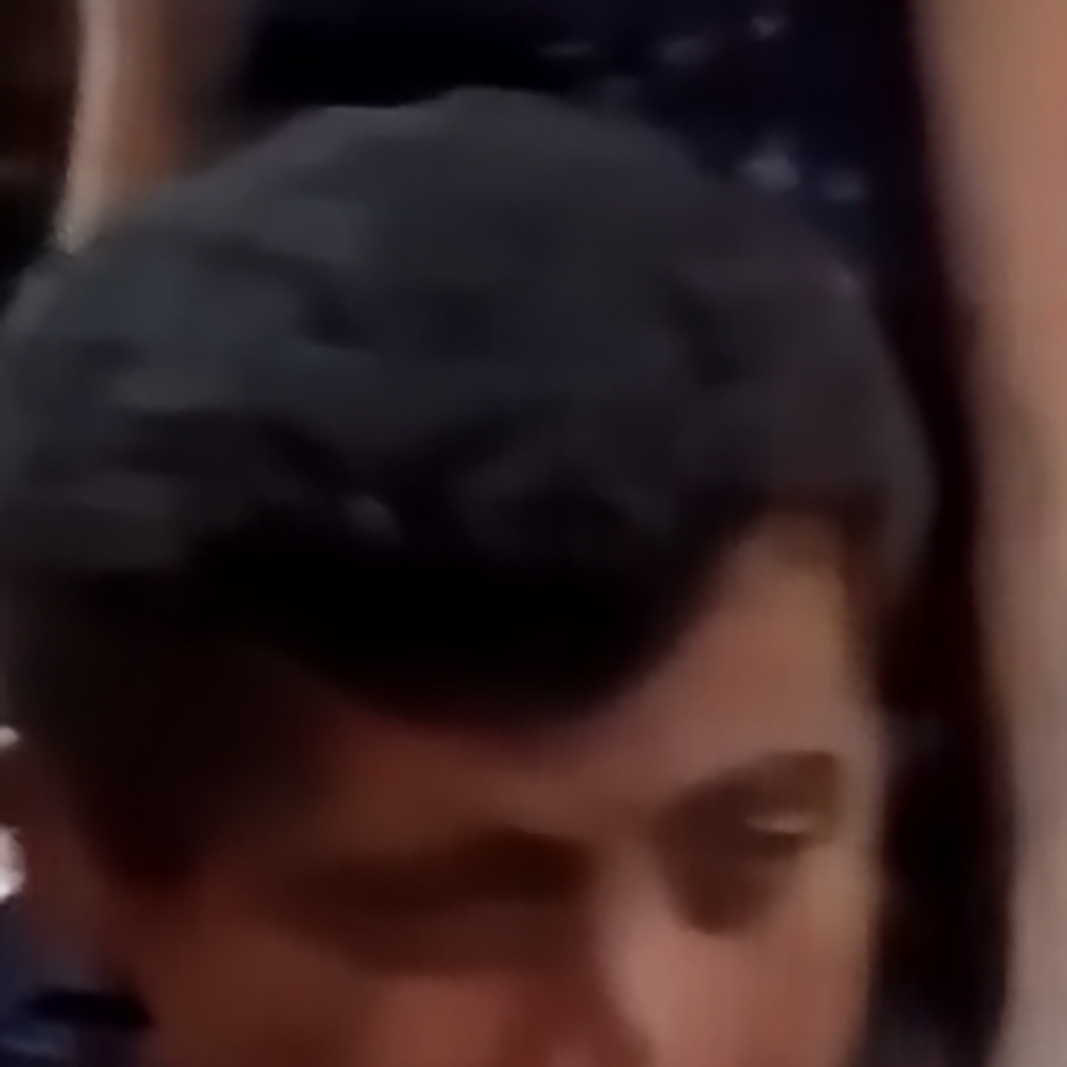
\includegraphics[width=1.3cm,height=1.3cm]{./gopro1/GOPR0384_11_05_004004_ours_3_5.png} &    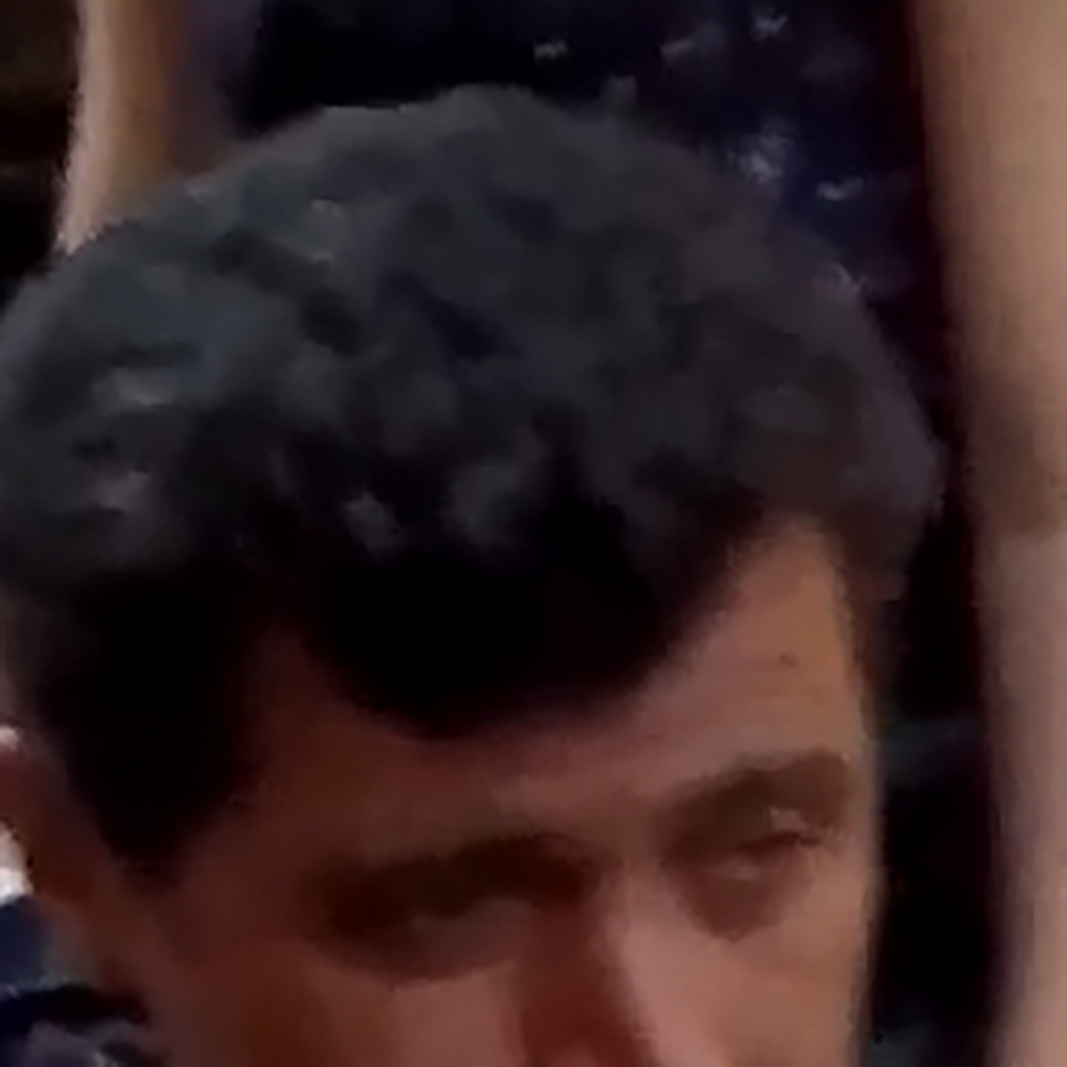
\includegraphics[width=1.3cm,height=1.3cm]{./gopro1/GOPR0384_11_05_004004_3_5_sharp.png}       \\
                \textcolor{black}{\cite{26}} & \textcolor{black}{Ours} & \textcolor{black}{sharp}
                
        \end{tabular}
        \caption{\textcolor{black}{The comparison of the results between the SOTA  methods with our proposed method on the GOPRO dataset.}}
        \label{figure9}
        \vspace{-0.5em}
\end{figure}

\begin{figure}
        \center
        \scriptsize
        \begin{tabular}{ccc}
                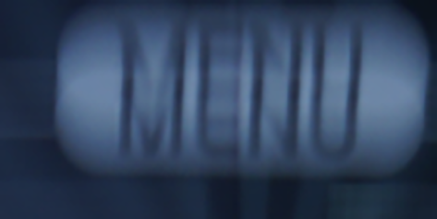
\includegraphics[width=2cm]{./compare_image/blur.png} &    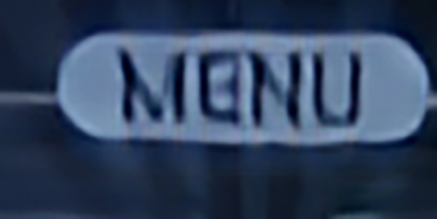
\includegraphics[width=2cm]{./compare_image/DG2.png} &    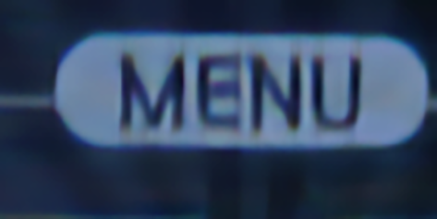
\includegraphics[width=2cm]{./compare_image/SRN.png}       \\
                \textcolor{black}{blur} & \textcolor{black}{DeblurGAN-v2} & \textcolor{black}{SRN} \\
                
                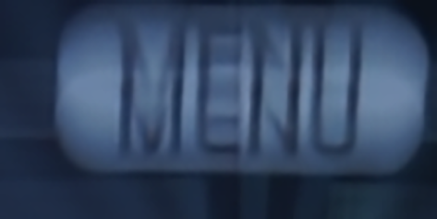
\includegraphics[width=2cm]{./compare_image/DMPHN.png} &    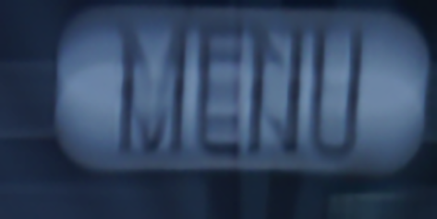
\includegraphics[width=2cm]{./compare_image/MIMO.png} &    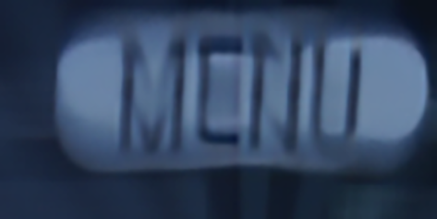
\includegraphics[width=2cm]{./compare_image/MPR.png}       \\
                \textcolor{black}{DMPHN} & \textcolor{black}{MIMO-UNet+} & \textcolor{black}{MPRNet} \\
                
                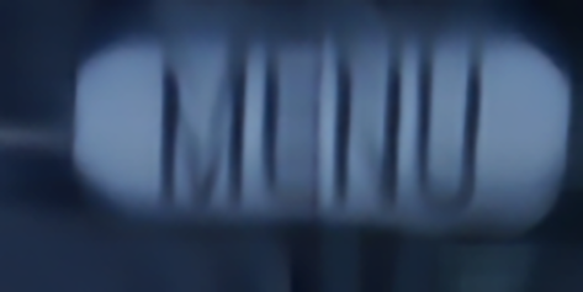
\includegraphics[width=2cm]{./compare_image/blur_AD.png} & 
                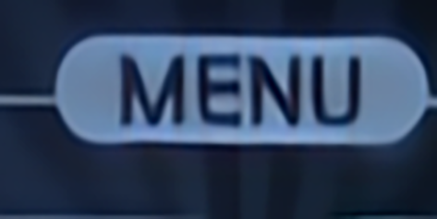
\includegraphics[width=2cm]{./compare_image/ours.png} &    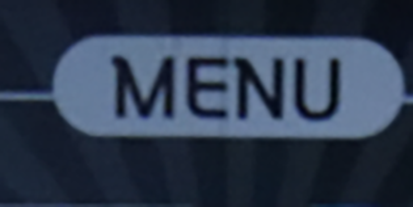
\includegraphics[width=2cm]{./compare_image/GT.png}       \\
                \textcolor{black}{\cite{26}} & \textcolor{black}{Ours} & \textcolor{black}{sharp}
                
        \end{tabular}
        \caption{\textcolor{black}{The comparison of the results between the SOTA  methods with our proposed method on the RealBlur dataset.}}
        \label{figure10}
        \vspace{-0.5em}
\end{figure}

\begin{figure}
        \center
        \scriptsize
        \begin{tabular}{ccc}
                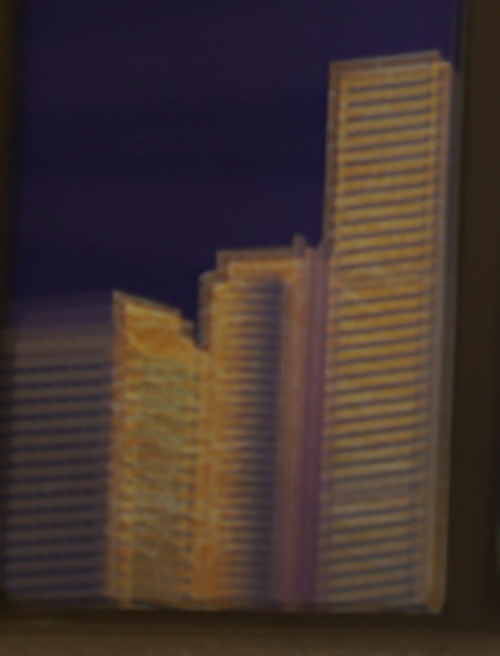
\includegraphics[width=1.3cm]{./compare_image/blur1.png} &    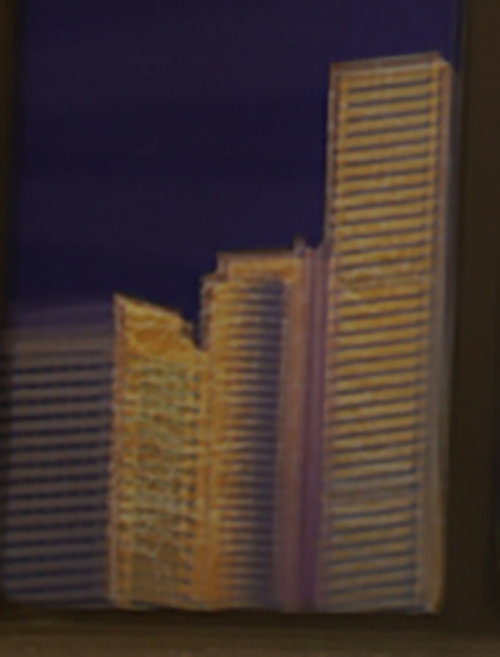
\includegraphics[width=1.3cm]{./compare_image/DG21.png} &    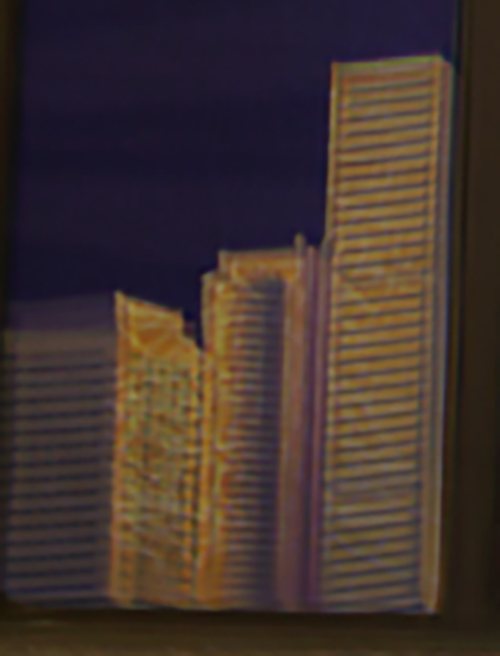
\includegraphics[width=1.3cm]{./compare_image/SRN1.png}       \\
                \textcolor{black}{blur} & \textcolor{black}{DeblurGAN-v2} & \textcolor{black}{SRN} \\
                
                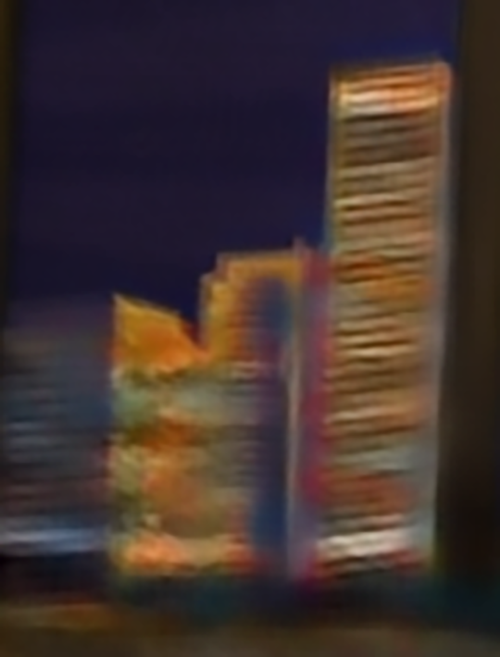
\includegraphics[width=1.3cm]{./compare_image/DMPHN1.png} &    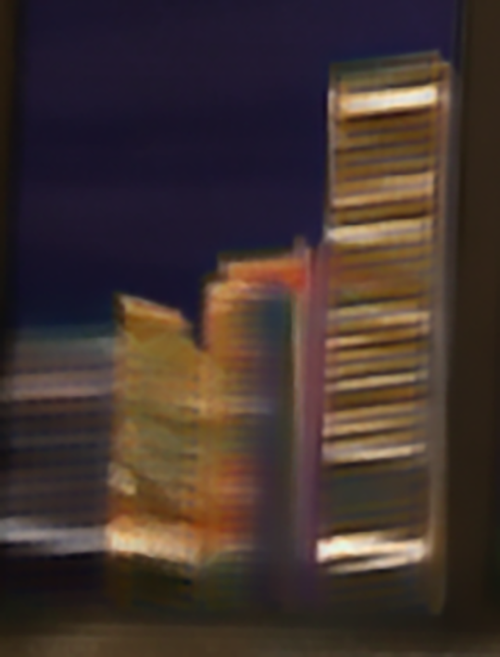
\includegraphics[width=1.3cm]{./compare_image/MIMO1.png} &    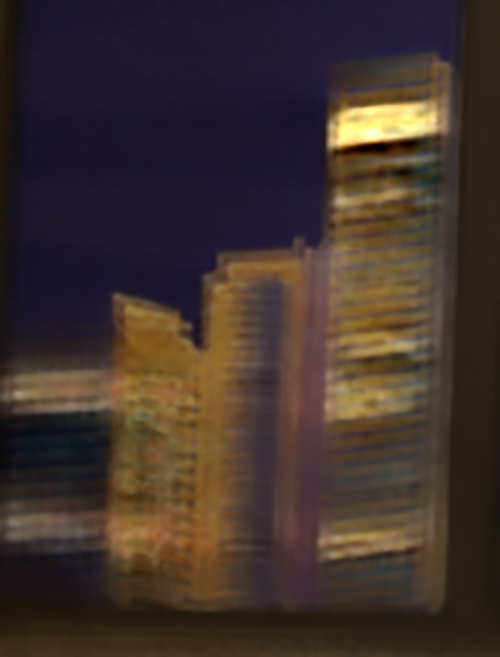
\includegraphics[width=1.3cm]{./compare_image/MPR1.png}       \\
                \textcolor{black}{DMPHN} & \textcolor{black}{MIMO-UNet+} & \textcolor{black}{MPRNet} \\
                

                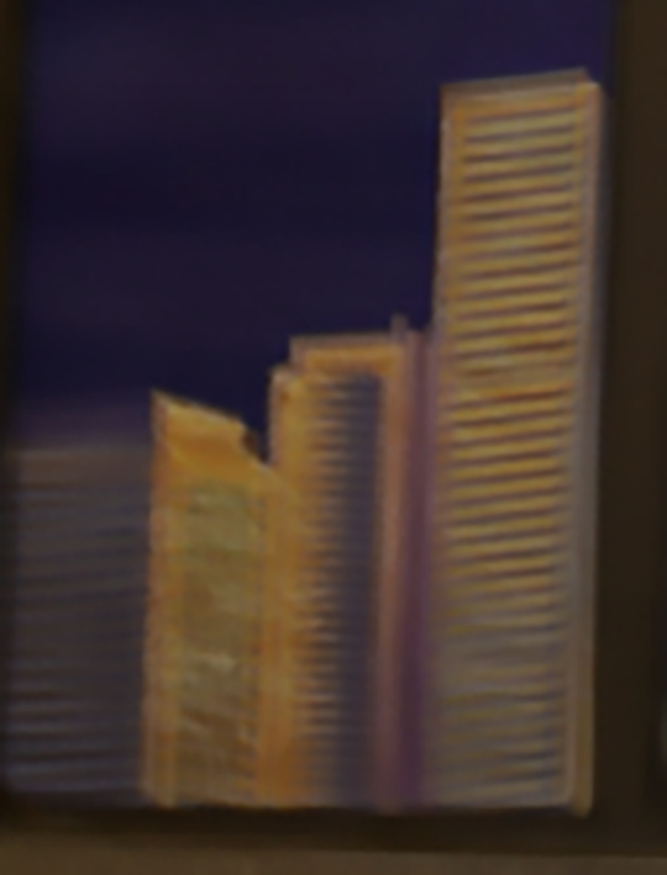
\includegraphics[width=1.3cm]{./compare_image/blur1_AD.png} &
                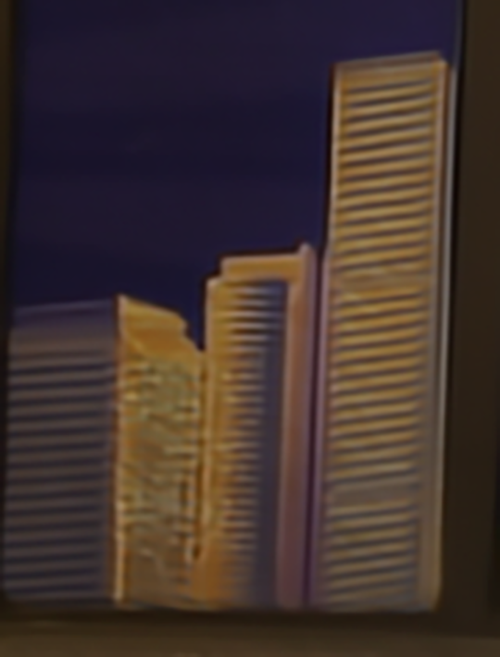
\includegraphics[width=1.3cm]{./compare_image/ours1.png} &    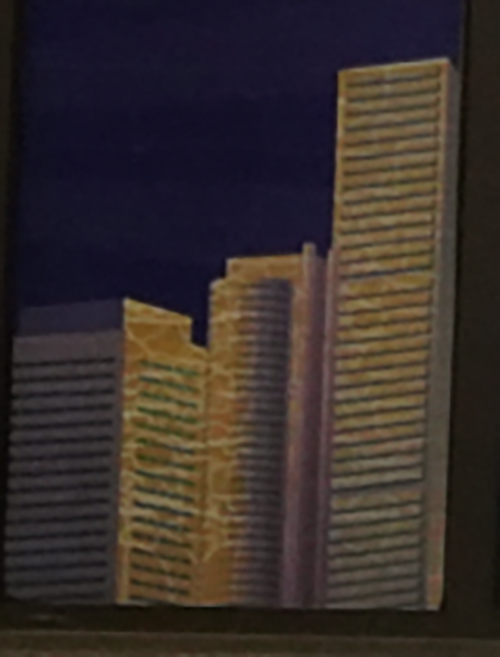
\includegraphics[width=1.3cm]{./compare_image/GT1.png}       \\
                \textcolor{black}{\cite{26}} & \textcolor{black}{Ours} & \textcolor{black}{sharp}
                
        \end{tabular}
        \caption{\textcolor{black}{The comparison of the results between the SOTA  methods with our proposed method on the RealBlur dataset.}}
        \label{figure11}
        \vspace{-0.5em}
\end{figure}

\begin{figure}
        \center
        \scriptsize
        \begin{tabular}{ccc}
                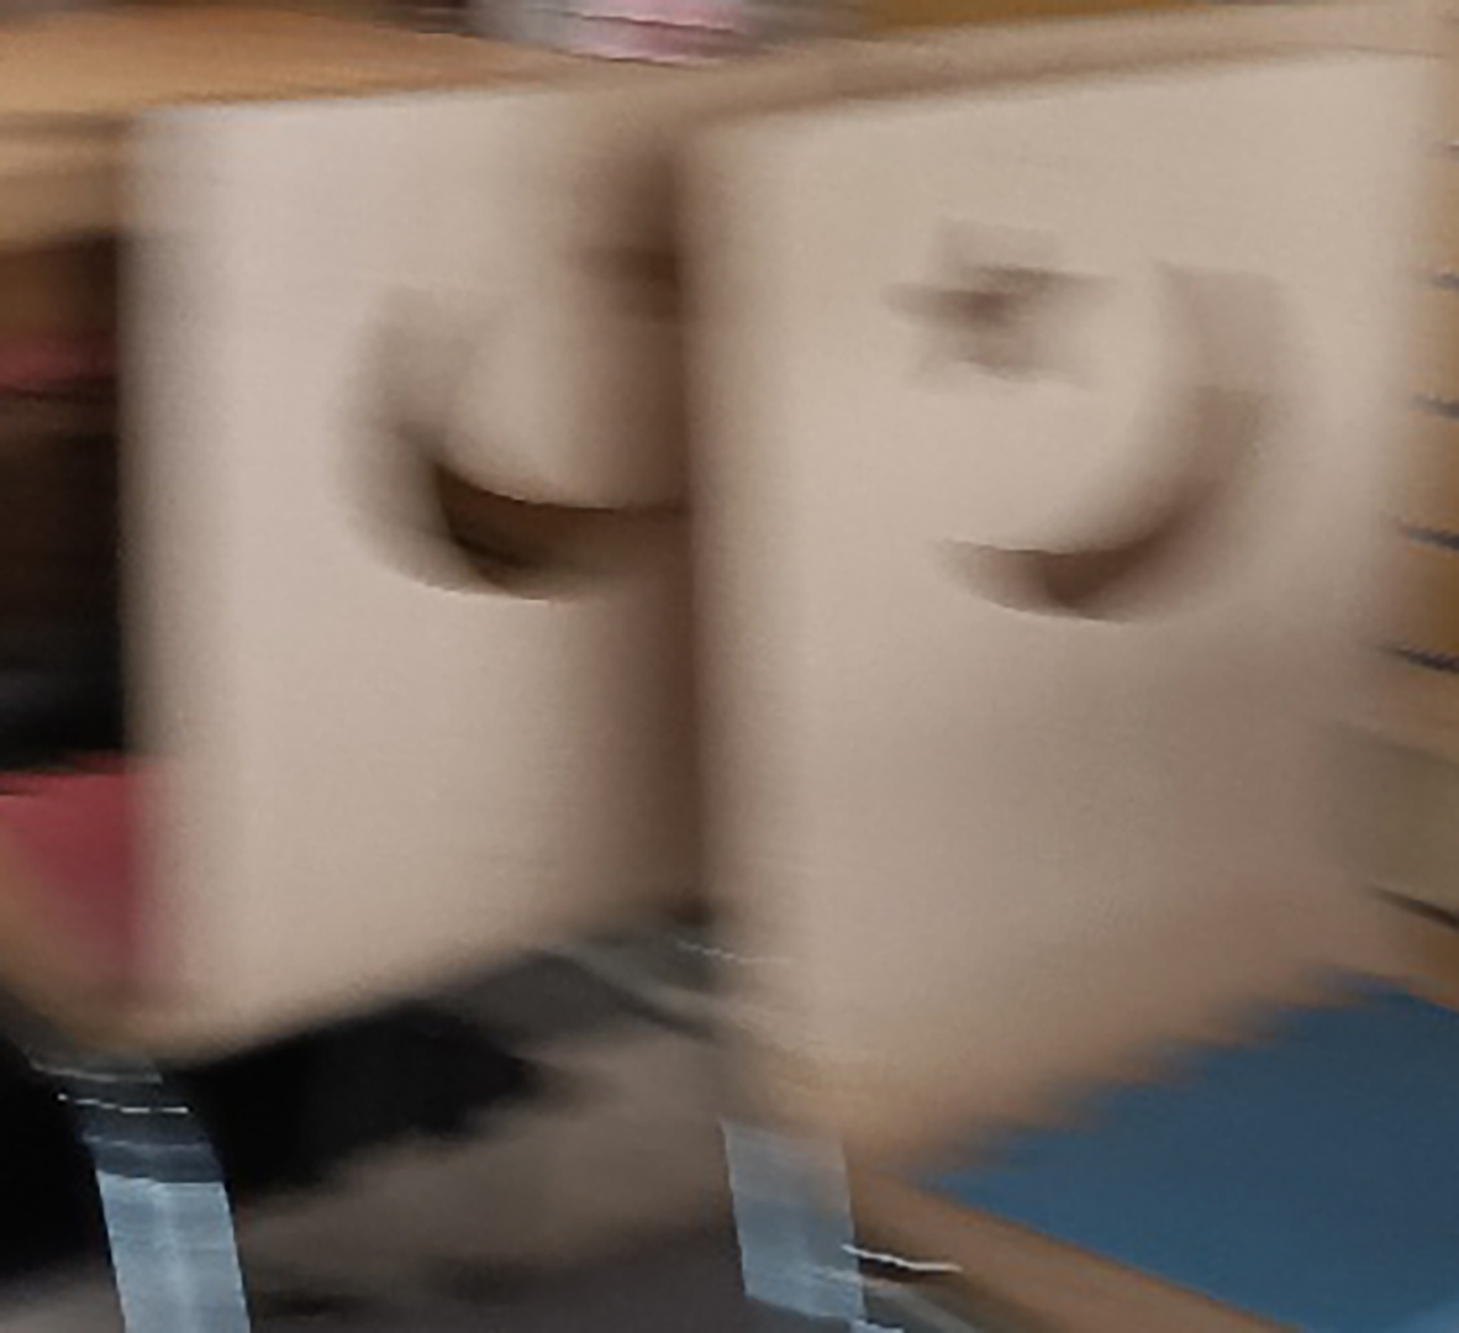
\includegraphics[width=1.3cm,height=1.3cm]{./real/000003_blur_patch.png} &    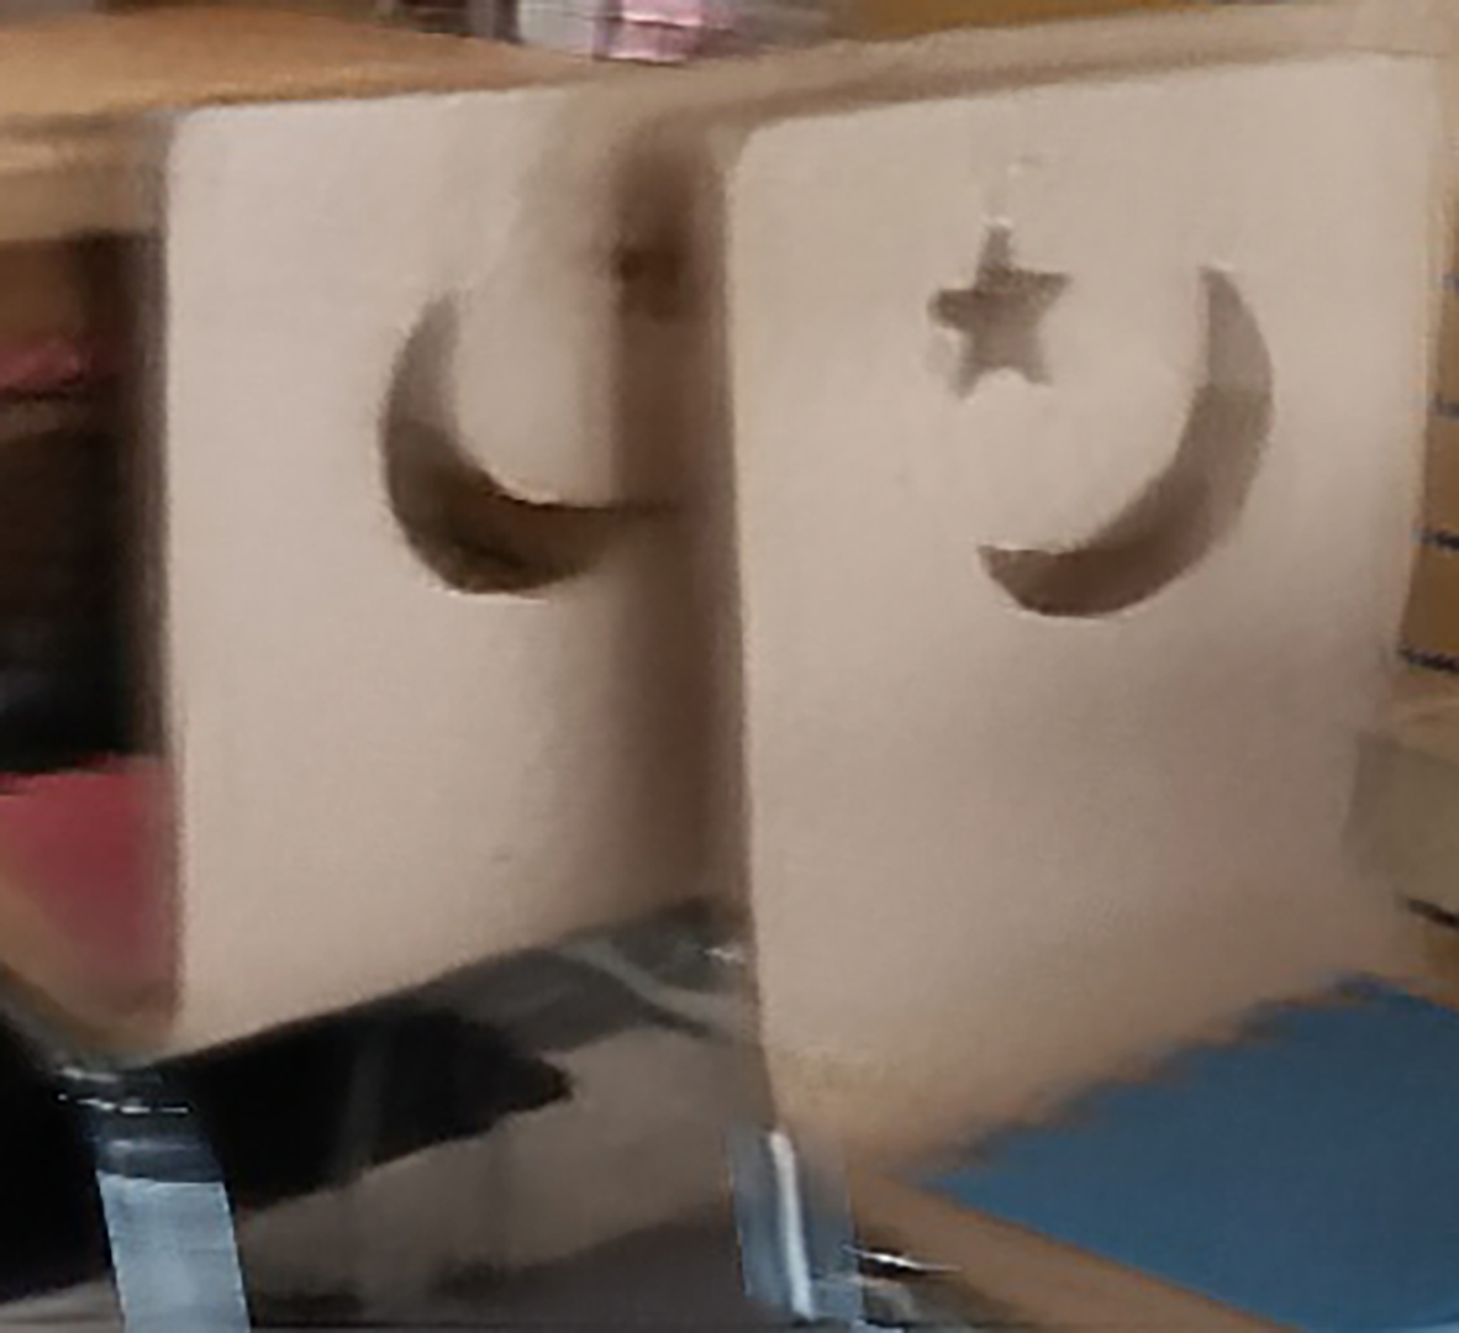
\includegraphics[width=1.3cm,height=1.3cm]{./real/000003_blur_D-GAN2_patch.png} &    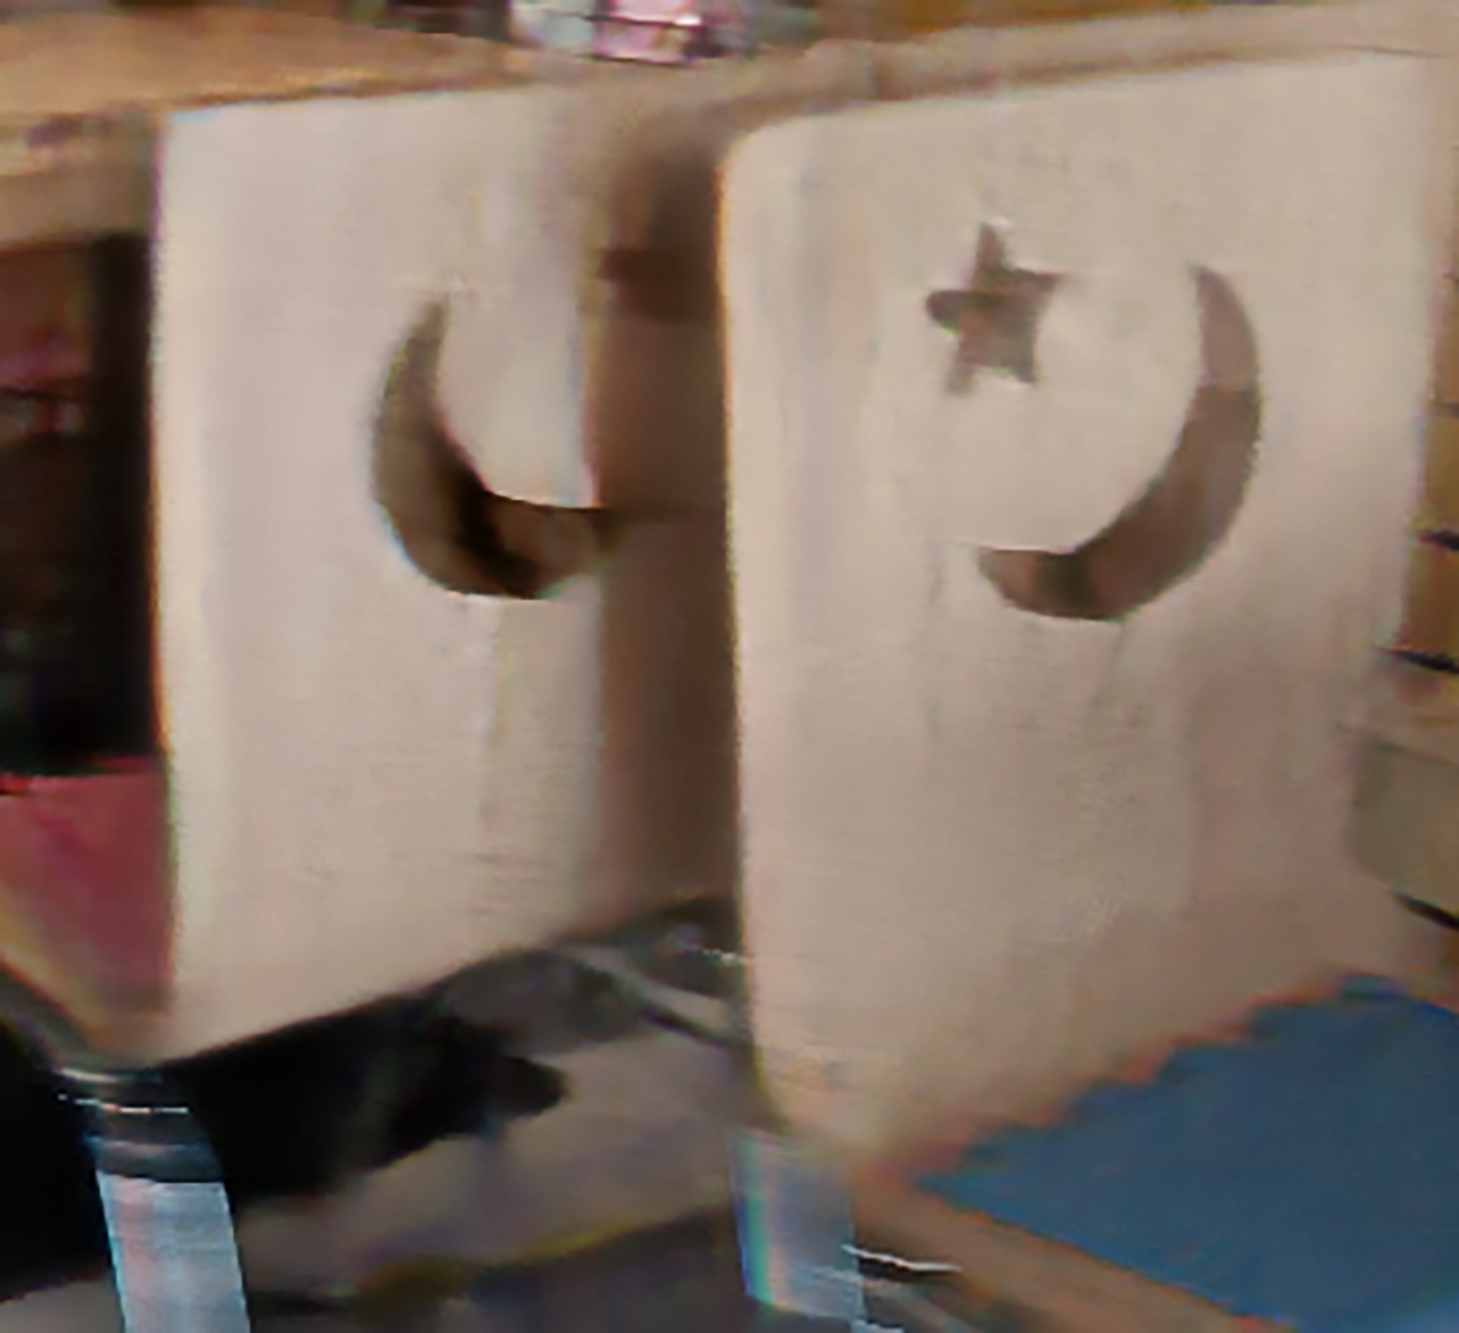
\includegraphics[width=1.3cm,height=1.3cm]{./real/000003_blur_SRN_patch.png}       \\
                blur & DeblurGAN-v2 & SRN \\
                
                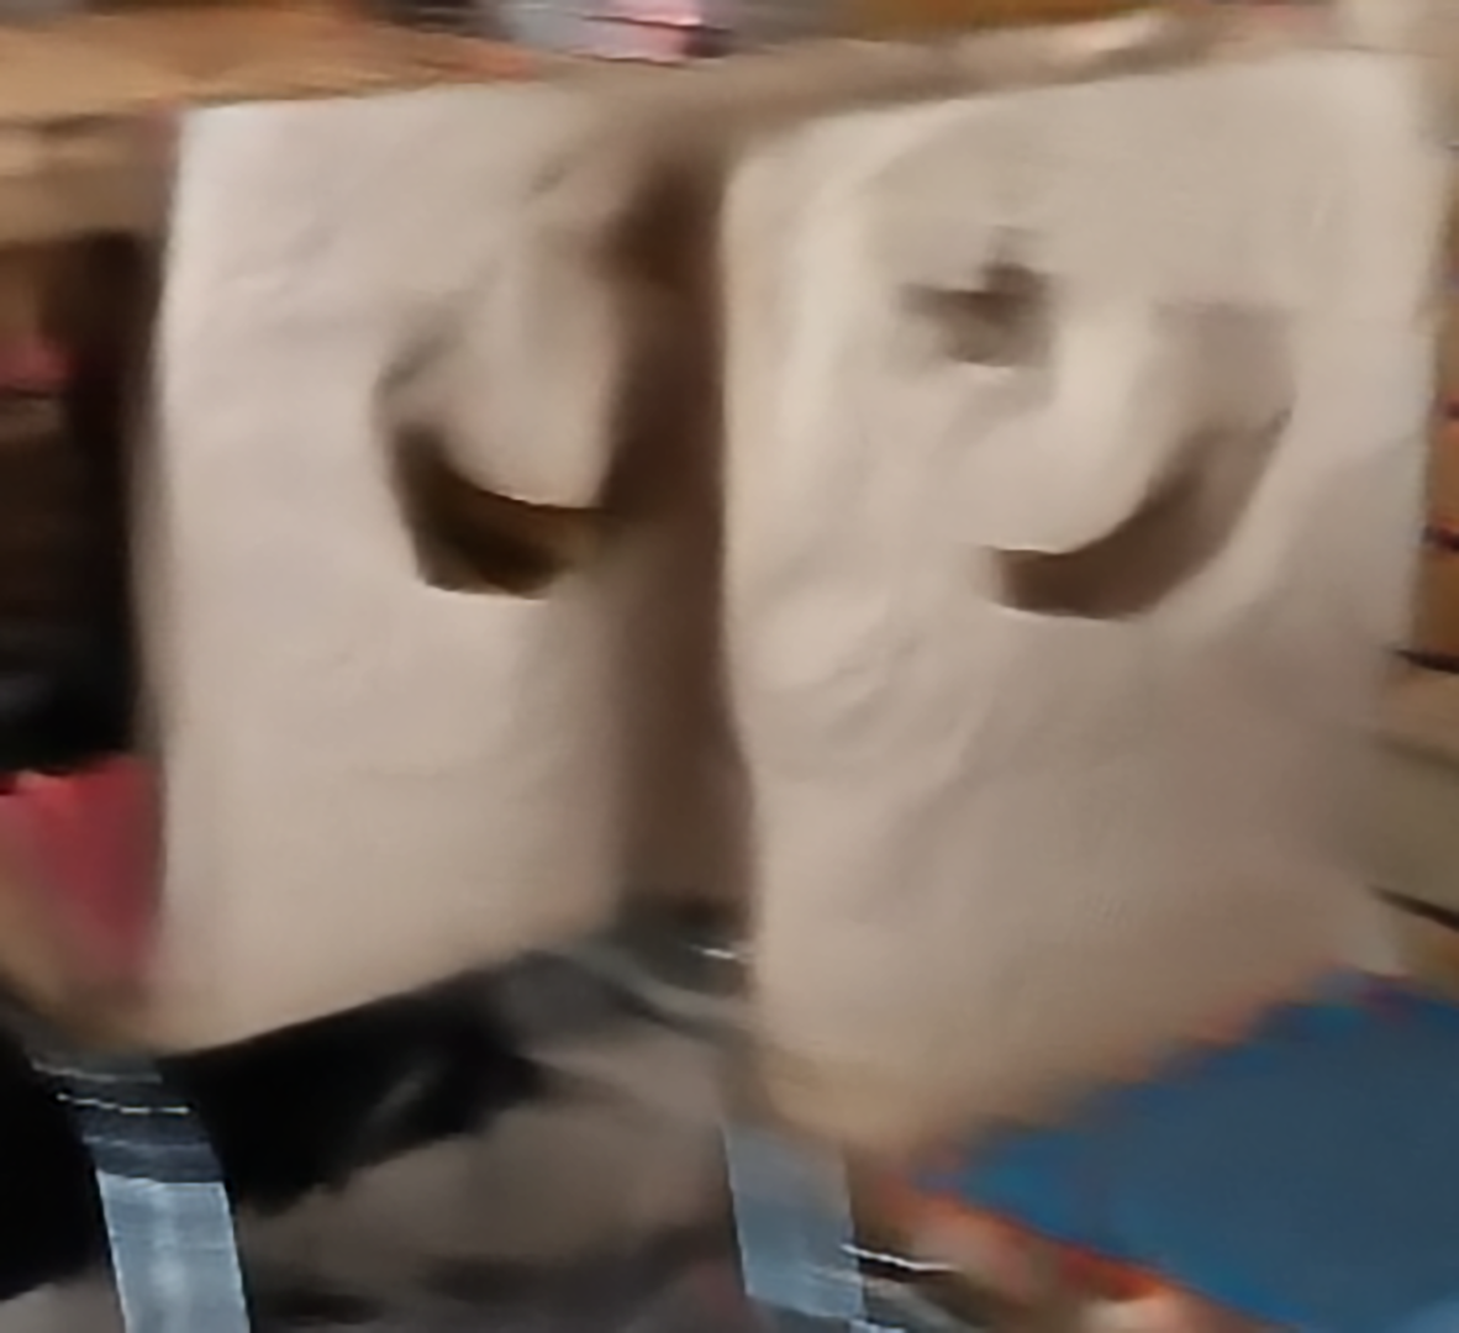
\includegraphics[width=1.3cm,height=1.3cm]{./real/000003_blur_DMPHN_patch.png} &  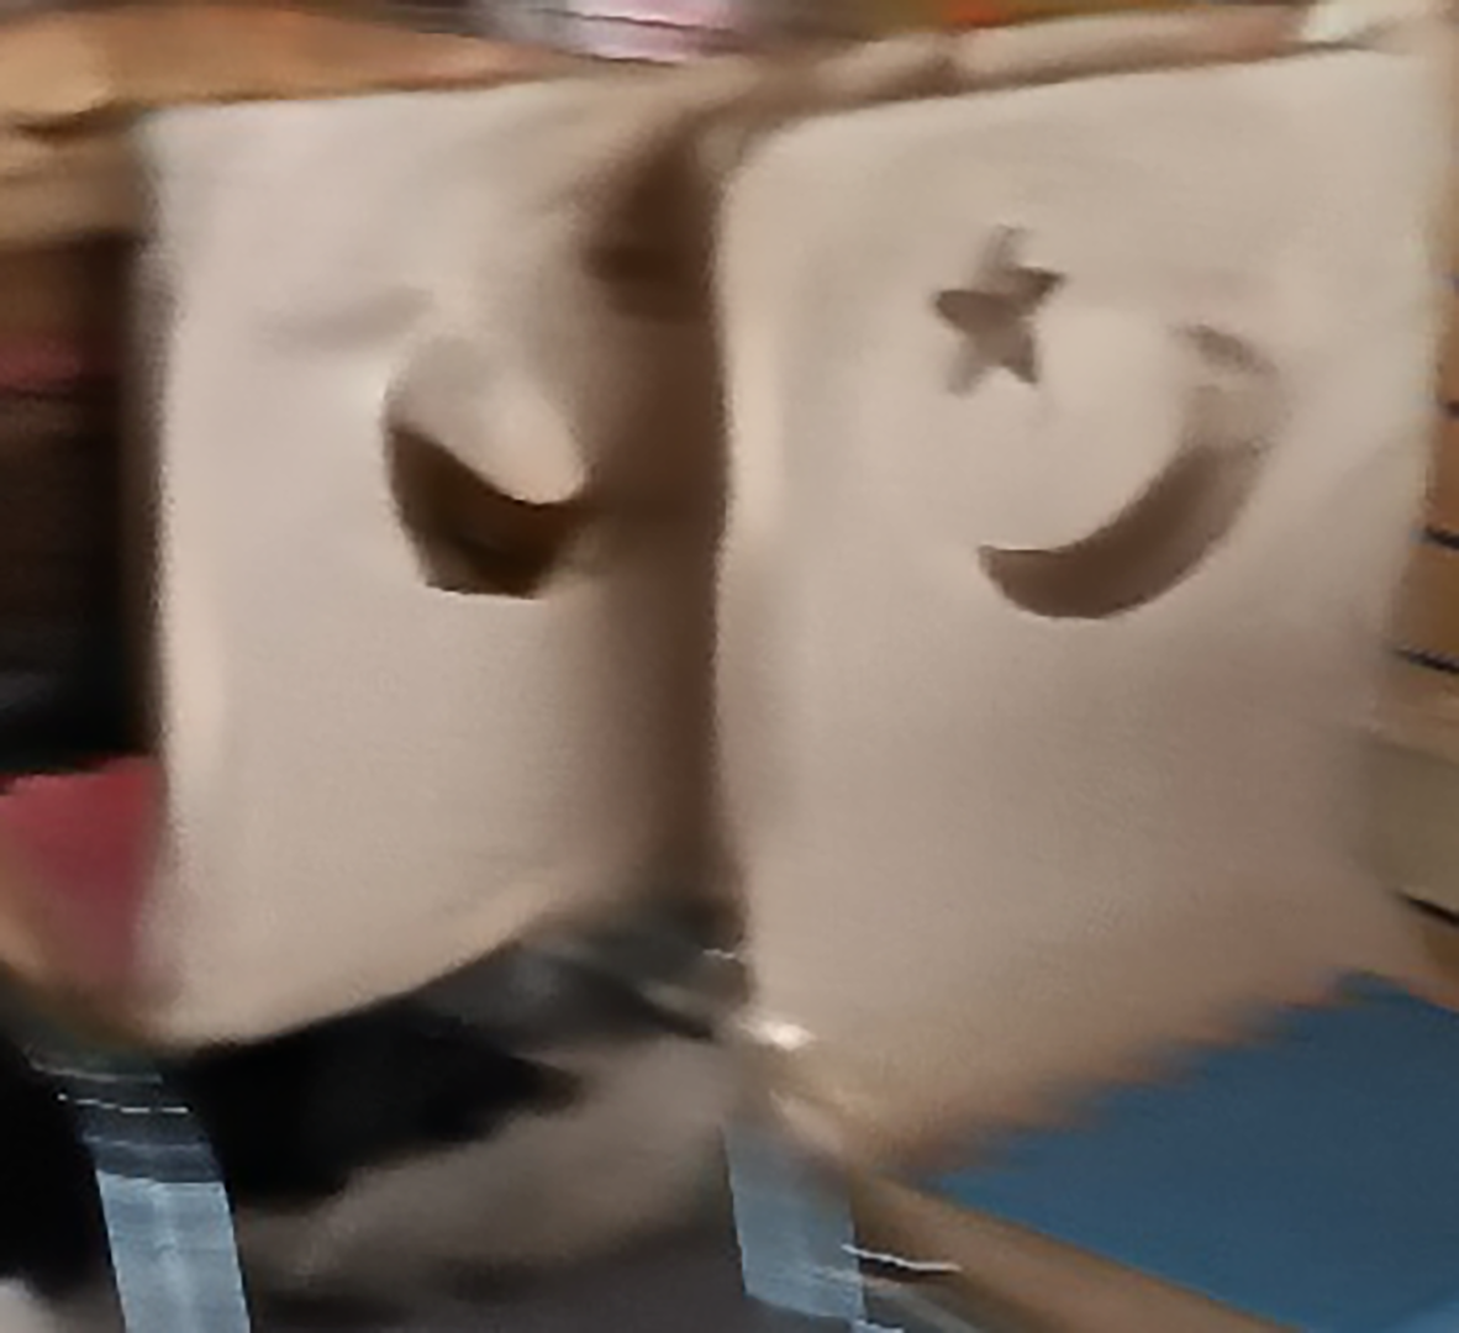
\includegraphics[width=1.3cm,height=1.3cm]{./real/000003_blur_MIMO_patch.png} &    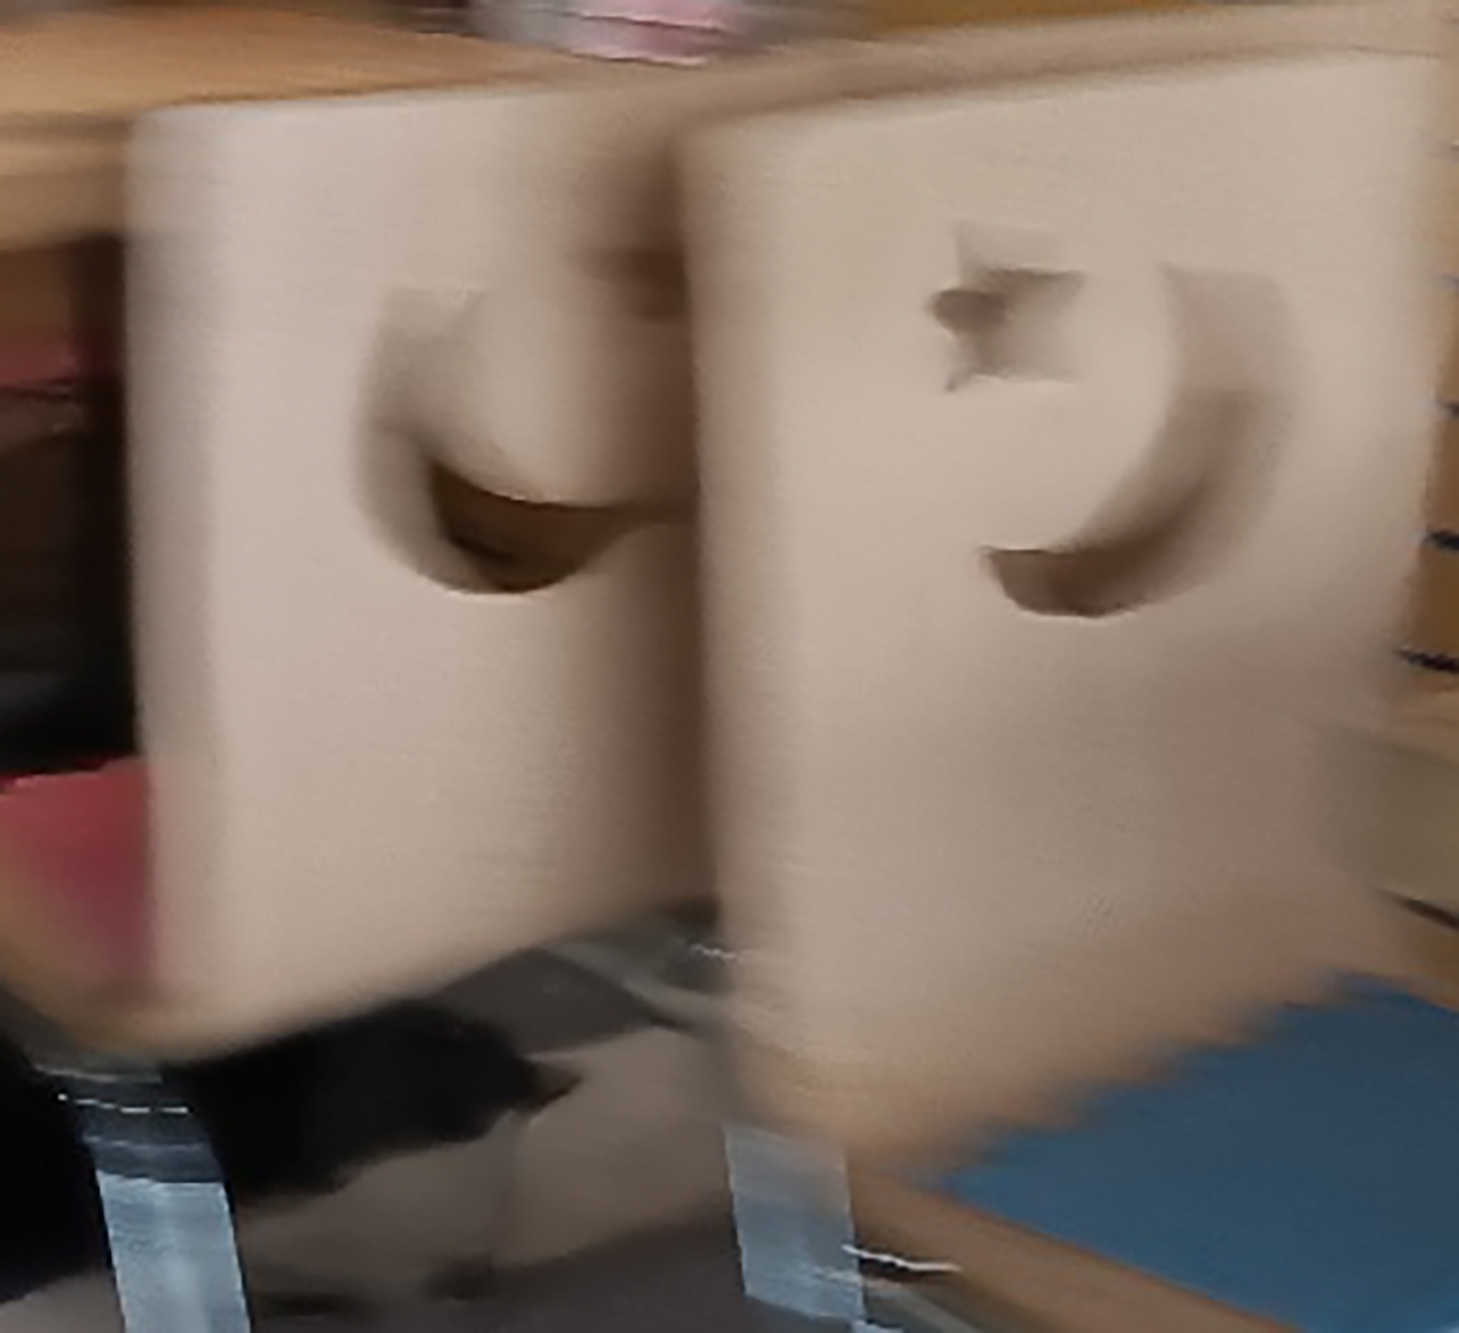
\includegraphics[width=1.3cm,height=1.3cm]{./real/000003_MPRNet_patch.png}       \\
                DMPHN & MIMO-UNet+ & MPRNet \\
                

                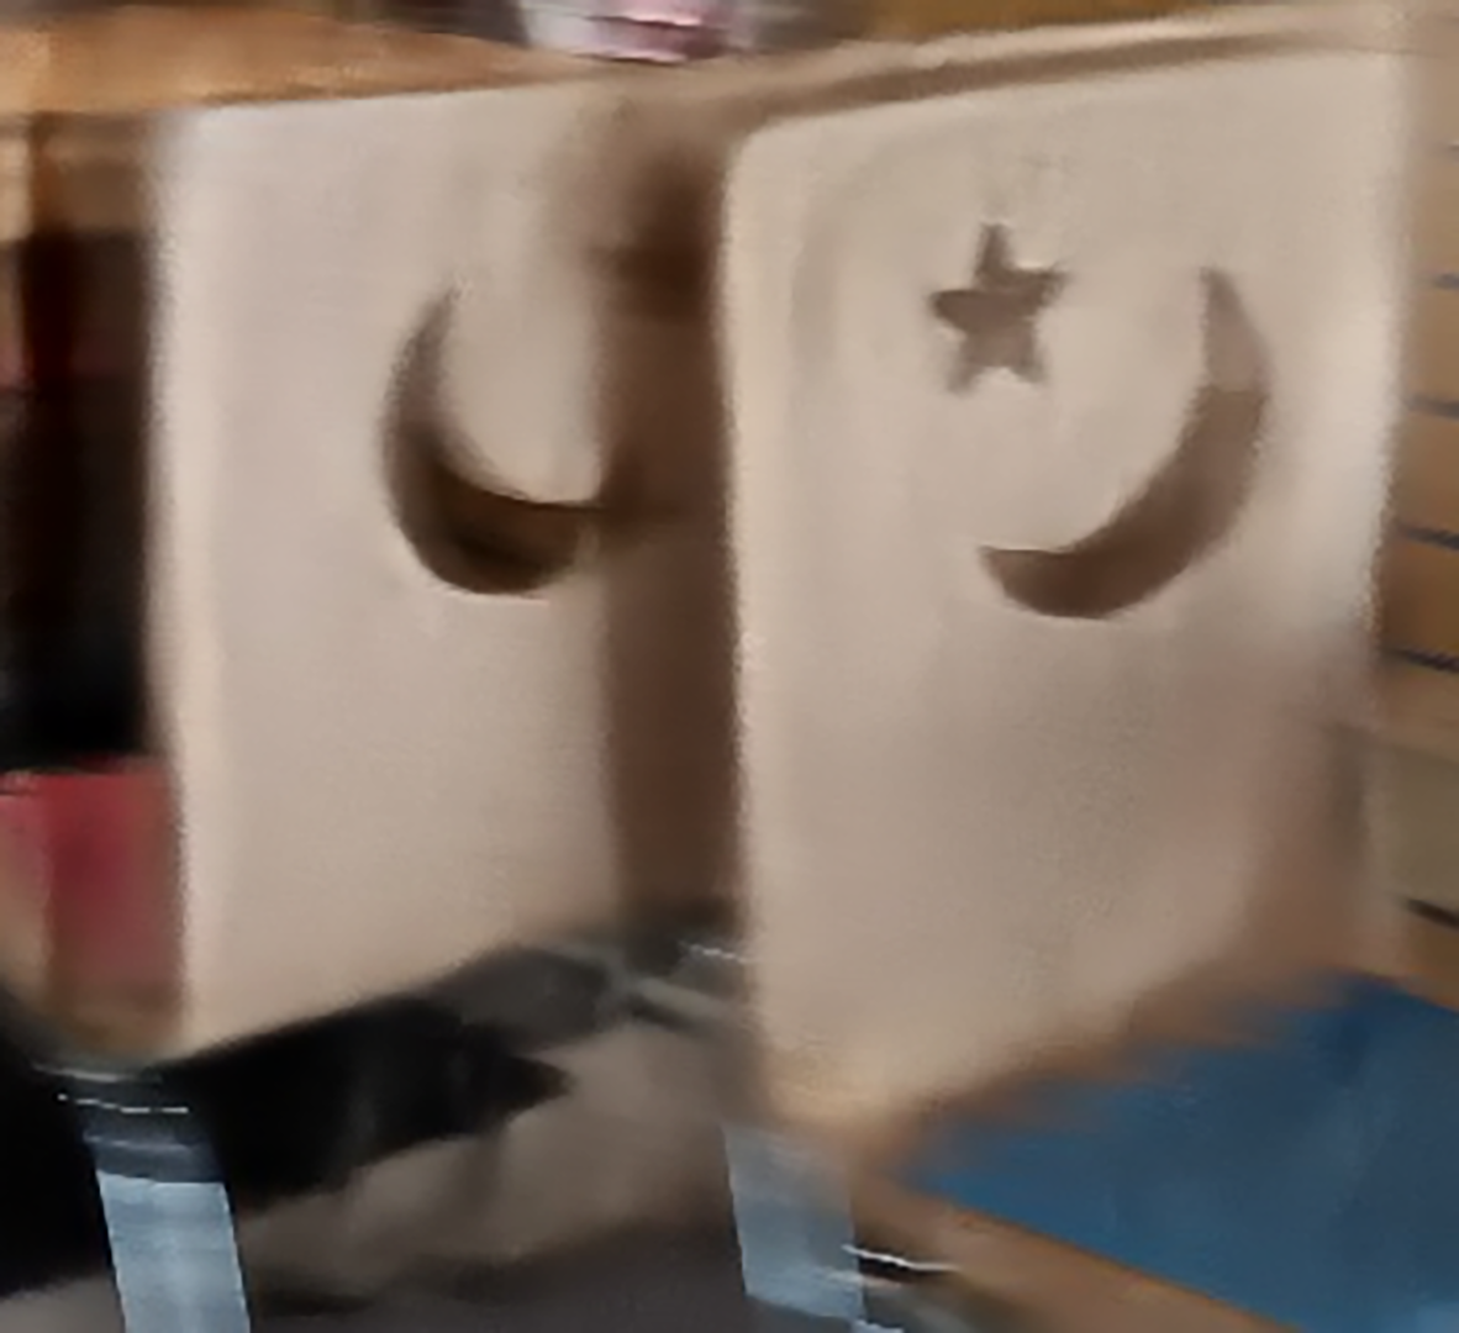
\includegraphics[width=1.3cm,height=1.3cm]{./real/000003_blur_patch_AD.png} & 
                \includegraphics[width=1.3cm,height=1.3cm]{./real/000003_blur_2500_Self_Deblur_patch.png} &    
                \includegraphics[width=1.3cm,height=1.3cm]{./real/000003_ours_patch.png}       \\
                \textcolor{black}{\cite{26}} & Self-Deblur & Ours \\
                
        \end{tabular}
        \caption{The comparison of the results between the SOTA methods with our proposed method on real-shot blurry images.}
        \label{figure12}
        \vspace{-0.5em}
\end{figure}
\subsubsection{The effectiveness of EGN}
We first compared the experimental results of the network with and without EGN. Secondly, HSIC\cite{10} is used to evaluate the correlation between the images and the feature maps in the middle layer of the network, which proves the effectiveness of EGN.

For the input feature maps of the last convolutional layer, we use HSIC as an independent metric to evaluate the correlation between the feature maps and the images. In TABLE 5, the correlation between the feature maps and the blurry image is set to 1, so the HSIC value of the sharp image is greater than 1, indicating that correlation between the feature maps and the sharp image is higher.

As can be seen from TABLE 4 and TABLE 5, after the introduction of EGN, the network performance has been significantly improved and the similarity between the feature maps and the sharp image will be significantly improved, which is the main reason why the introduction of EGN is effective for image deblurring.


\subsubsection{The effectiveness of Gradient Loss}
We performed ablation study of the proposed gradient loss, which was trained on the GOPRO dataset and then tested on the RealBlur dataset. The quantitative results are shown in TABLE 6. The representative visualization results are shown in Figure 13 and Figure 14.

As can be seen from TABLE 6, Figure 13 and Figure 14, after the introduction of Gradient Loss, the network has better generalization ability.

\begin{table}[!t]
% increase table row spacing, adjust to taste
\renewcommand{\arraystretch}{1.3}

\caption{\textcolor{black}{The comparison of the results with and without Gradient Loss.}
}
\label{table6}
\centering
% Some packages, such as MDW tools, offer better commands for making tables
% than the plain LaTeX2e tabular which is used here.
\begin{tabular}{ccc}
\hline\noalign{\smallskip}
 & \textcolor{black}{PSNR(R-R/R-J)} & \textcolor{black}{SSIM(R-R/R-J)}  \\
\noalign{\smallskip}\hline\noalign{\smallskip}
\textcolor{black}{w/o Gradient Loss} & \textcolor{black}{33.7142/26.3708} & \textcolor{black}{0.9464/0.8617} \\

\textcolor{black}{w Gradient Loss} & \textcolor{black}{34.2960/26.9638} & \textcolor{black}{0.9520/0.8765} \\

\noalign{\smallskip}\hline
\end{tabular}
\end{table}


\begin{figure}
        \center
        \scriptsize
        \begin{tabular}{cccc}
                \includegraphics[width=1.5cm]{./loss/blur.png} &    \includegraphics[width=1.5cm]{./loss/wo.png}  &
                 \includegraphics[width=1.5cm]{./loss/w.png} &    \includegraphics[width=1.5cm]{./loss/GT.png}\\
                \textcolor{black}{blur} & \textcolor{black}{w/o Gradient Loss} &  \textcolor{black}{with Gradient Loss} & \textcolor{black}{sharp}\\
                
        \end{tabular}
        
        \caption{\textcolor{black}{The results of the ablation study of the Gradient Loss on the RealBlur dataset.}}
        \label{figure13}
        \vspace{-0.5em}
\end{figure}

\begin{figure}
        \center
        \scriptsize
        \begin{tabular}{ccc}
                \includegraphics[width=2.3cm]{./loss/blur1.png}  &
                \includegraphics[width=2.3cm]{./loss/wo1.png} & 
                \includegraphics[width=2.3cm]{./loss/w1.png}  \\
                \textcolor{black}{blur} & \textcolor{black}{w/o Gradient Loss} &  \textcolor{black}{with Gradient Loss}\\
                
        \end{tabular}
        
        \caption{\textcolor{black}{The  results of the ablation study of the Gradient Loss on real-shot blurry images.}}
        \label{figure14}
        \vspace{-0.5em}
\end{figure}

\section{Conclusion}
In this paper, a novel image deblurring method based on Enhanced Gradient Network(EGN) is presented. The proposed EGN can increase the proportion of gradient information in the feature maps and improve the correlation between the feature maps and the sharp image. It can also eliminate the artifacts and retain the sharp details. In order to fuse multiple test results and recover more edge details, we further propose a self-ensemble network and redesign the loss functions. It can get better ensemble results than the other self-ensemble methods. The experiments implemented on public datasets and real blurry images demonstrate that our proposed method achieves the state-of-the-art results in both qualitative and quantitative ways.



% Authors must disclose all relationships or interests that 
% could have direct or potential influence or impart bias on 
% the work: 
%
% \section*{Conflict of interest}
%
% The authors declare that they have no conflict of interest.


% BibTeX users please use one of
%\bibliographystyle{spbasic}      % basic style, author-year citations
%\bibliographystyle{spmpsci}      % mathematics and physical sciences
%\bibliographystyle{spphys}       % APS-like style for physics
%\bibliography{}   % name your BibTeX data base

% Non-BibTeX users please use
% \begin{thebibliography}{}
% %
% % and use \bibitem to create references. Consult the Instructions
% % for authors for reference list style.
% %
% \bibitem{RefJ}
% % Format for Journal Reference
% Author, Article title, Journal, Volume, page numbers (year)
% % Format for books
% \bibitem{RefB}
% Author, Book title, page numbers. Publisher, place (year)
% etc
% \end{thebibliography}


\section*{Acknowledgements }
This work was supported by the Natural Science Foundation of Heilongjiang Province, China, under Grant LH2021F026 and Fundamental Research Funds for the Central Universities under Grant HIT.NSRIF202243.


%\bibliographystyle{spphys}
%\bibliographystyle{unsrt}
\begin{thebibliography}{27}
	\bibitem{1}Carbajal, Guillermo, et al. "Single image non-uniform blur kernel estimation via adaptive basis decomposition." Computing Research Repository (CoRR), arXiv: 2102.01026, pp. 1-11, feb 2021 (2021).
	\bibitem{2}Boden, A. F., et al. "Massively parallel spatially variant maximum-likelihood restoration of Hubble Space Telescope imagery." JOSA A 13.7 (1996): 1537-1545.
	\bibitem{3}Nah, Seungjun, Tae Hyun Kim, and Kyoung Mu Lee. "Deep multi-scale convolutional neural network for dynamic scene deblurring." Proceedings of the IEEE conference on computer vision and pattern recognition. 2017.
	\bibitem{4}Tao, Xin, et al. "Scale-recurrent network for deep image deblurring." Proceedings of the IEEE conference on computer vision and pattern recognition. 2018.
	\bibitem{5}Gao, Hongyun, et al. "Dynamic scene deblurring with parameter selective sharing and nested skip connections." Proceedings of the IEEE/CVF conference on computer vision and pattern recognition. 2019.
	\bibitem{6}Zhang, Hongguang, et al. "Deep stacked hierarchical multi-patch network for image deblurring." Proceedings of the IEEE/CVF Conference on Computer Vision and Pattern Recognition. 2019.
	\bibitem{7}Zamir, Syed Waqas, et al. "Multi-stage progressive image restoration." Proceedings of the IEEE/CVF conference on computer vision and pattern recognition. 2021.
	\bibitem{8}Mao, Xintian, et al. "Deep residual fourier transformation for single image deblurring." arXiv preprint arXiv:2111.11745 (2021).
	\bibitem{9}Cho, Sung-Jin, et al. "Rethinking coarse-to-fine approach in single image deblurring." Proceedings of the IEEE/CVF international conference on computer vision. 2021.
	\bibitem{10}Ma, Wan-Duo Kurt, J. P. Lewis, and W. Bastiaan Kleijn. "The HSIC bottleneck: Deep learning without back-propagation." Proceedings of the AAAI Conference on Artificial Intelligence. Vol. 34. No. 04. 2020.
	\bibitem{11}Quan, Yuhui, Zicong Wu, and Hui Ji. "Gaussian Kernel Mixture Network for Single Image Defocus Deblurring." Advances in Neural Information Processing Systems 34 (2021): 20812-20824.
	\bibitem{12}Quan, Yuhui, et al. "Nonblind image deblurring via deep learning in complex field." IEEE Transactions on Neural Networks and Learning Systems (2021).
	\bibitem{13}Chen, Mingqin, et al. "Nonblind Image Deconvolution via Leveraging Model Uncertainty in An Untrained Deep Neural Network." International Journal of Computer Vision (2022): 1-20.
	\bibitem{14}Quan, Yuhui, Hui Ji, and Zuowei Shen. "Data-driven multi-scale non-local wavelet frame construction and image recovery." Journal of Scientific Computing 63.2 (2015): 307-329.
	\bibitem{15}Goodfellow, Ian, et al. "Generative adversarial networks." Communications of the ACM 63.11 (2020): 139-144.
	\bibitem{16}Gulrajani, Ishaan, et al. "Improved training of wasserstein gans." Advances in neural information processing systems 30 (2017).
	\bibitem{17}Kupyn, Orest, et al. "Deblurgan: Blind motion deblurring using conditional adversarial networks." Proceedings of the IEEE conference on computer vision and pattern recognition. 2018.
	\bibitem{18}Kupyn, Orest, et al. "Deblurgan-v2: Deblurring (orders-of-magnitude) faster and better." Proceedings of the IEEE/CVF International Conference on Computer Vision. 2019.
	\bibitem{19}Hu, Jie, Li Shen, and Gang Sun. "Squeeze-and-excitation networks." Proceedings of the IEEE conference on computer vision and pattern recognition. 2018.
	\bibitem{20}Xie, Saining, et al. "Aggregated residual transformations for deep neural networks." Proceedings of the IEEE conference on computer vision and pattern recognition. 2017.
	\bibitem{21}Lim, Bee, et al. "Enhanced deep residual networks for single image super-resolution." Proceedings of the IEEE conference on computer vision and pattern recognition workshops. 2017.
	\bibitem{22}Chen, Mingqin, et al. "Self-Supervised Blind Image Deconvolution via Deep Generative Ensemble Learning." IEEE Transactions on Circuits and Systems for Video Technology (2022).
	\bibitem{23}Quan, Yuhui, et al. "Learning Deep Non-blind Image Deconvolution Without Ground Truths." European Conference on Computer Vision. Springer, Cham, 2022.
	\bibitem{24}Woo, Sanghyun, et al. "Cbam: Convolutional block attention module." Proceedings of the European conference on computer vision (ECCV). 2018.
	\bibitem{25}Rim, Jaesung, et al. "Real-world blur dataset for learning and benchmarking deblurring algorithms." European Conference on Computer Vision. Springer, Cham, 2020.
	\bibitem{26}Xu, Yong, et al. "Attentive deep network for blind motion deblurring on dynamic scenes." Computer Vision and Image Understanding 205 (2021): 103169.
	\bibitem{27}Wang, Chien-Yao, I-Hau Yeh, and Hong-Yuan Mark Liao. "You only learn one representation: Unified network for multiple tasks." arXiv preprint arXiv:2105.04206 (2021).
\end{thebibliography}

\def\bibfont{\fontsize{10.5}\selectfont}
% \bibliography{ref}
%\printbibliography
\twocolumn[
\begin{@twocolumnfalse}
\section*{\centering{\huge Declarations}}

\renewcommand{\labelitemi}{\textbullet}

\begin{itemize}

\setlength{\itemsep}{5pt}

\setlength{\parsep}{5pt}

\setlength{\parskip}{5pt}
\large \item \textbf{Ethics approval and consent to participate}

Not applicable

\item \textbf{Consent for publication}

Not applicable

\item \textbf{Availability of data and materials}

Not applicable

\item \textbf{Competing interests}

The authors declare that they have no competing interests.

\item \textbf{Funding}

This work was supported in part by the Natural Science Foundation of
Heilongjiang Province of China (No.LH2021F026) and Fundamental Research Funds for the Central Universities(No. HIT.NSRIF202243).

\item \textbf{Authors' contributions}

Changdi Zhao and Xiaoguang Di designed the research. Changdi Zhao drafted the manuscript. Xiaoguang Di helped organize the manuscript. Changdi Zhao, Xiaoguang Di and Feng Gao revised and finalized the paper.

\item \textbf{Acknowledgements}

We appreciated the Natural Science Foundation of Heilongjiang Province of China (No.LH2021F026) and Fundamental Research Funds for the Central
Universities(No. HIT.NSRIF202243) for their support.

\item \textbf{Authors' information (optional)}

\textbf{Changdi Zhao} received the B.S. degree in automation from Harbin Institute of Technology, China, in 2020. He is currently a graduate student at the Control and Simulation Center, Harbin Institute of Technology. His current research interests include deep learning, object detection and image restoration and enhancement.

\textbf{Xiaoguang Di} (corresponding author) is currently a Professor with the Control and Simulation Center, Harbin Institute of Technology. His current research interests include image restoration and enhancement, object detection and recognition, deep learning, and SLAM. He is a member of the Chinese Association of Automation and the China Simulation Federation.

\textbf{Feng Gao} received the B.S. degree in automation from Harbin Engineering University, China, in 2021. He is currently a graduate student at the Control and Simulation Center, Harbin Institute of Technology. His current research interests include deep learning, object detection and image restoration and enhancement.


\end{itemize}
\end{@twocolumnfalse}
]

\clearpage


\end{sloppypar}
%\bibliographystyle{spphys}
%\bibliography{ref}
\end{document}
% end of file template.tex

